%% Full length research paper template
%% Created by Simon Hengchen and Nilo Pedrazzini for the Journal of Open Humanities Data (https://openhumanitiesdata.metajnl.com)

\documentclass{article}
\usepackage{tabularx}
\usepackage[T1]{fontenc}
\usepackage[polish]{babel}
\usepackage[utf8]{inputenc}
\usepackage{lmodern}
\selectlanguage{polish}
\usepackage[utf8]{inputenc}
\usepackage{johd}
\usepackage{abstract}
\renewcommand{\abstractname}{} 
\addto{\captionspolish}{\renewcommand{\abstractname}{}}
\usepackage{graphicx}
\usepackage{caption}
\usepackage{subcaption}
\usepackage{amsmath}
\usepackage{xcolor}
\usepackage{multirow}
\usepackage{upgreek}
\usepackage{gensymb}
\usepackage[tmargin=2.5cm,bmargin=2.5cm,margin=2cm,rmargin=2cm]{geometry}

\title{Pytania na egzamin inżynierski}


\begin{document}

\maketitle

\section{Zasady względności Galileusza; układy inercjalne}

Układ inercjalny - układ ,w którym ciała, niepodlegające żadnemu zewnętrznemu oddziaływaniu z innymi ciałami, poruszają się ruchem jednostajnym prostoliniowym lub pozostają w spoczynku.  \\

\noindent Zasada względności - w dowolnym inercjalnym układzie odniesienia prawa mechaniki są takie same. 
Zasada względności Galileusza mówi, że niezależnie od tego, jaki układ inercjalny przyjmiemy, zawsze otrzymamy taki sam rodzaj ruchu. Inne sformułowanie tej zasady mówi, że wszystkie układy inercjalne są równoważne. \\

\noindent Układ inercjalny to taki układ, w którym jest słuszna pierwsza zasada dynamiki Newtona. Jeśli nie mielibyśmy pewności, a chcielibyśmy sprawdzić czy znajdujemy się w układzie inercjalnym moglibyśmy, np. rozrzucić kamienie. Jeżeli kamienie poruszały się po torach prostych ze stałą prędkością, wówczas znajdujemy się w układzie inercjalnym i wszystkie układy, które poruszają się względem naszego układu ze stałą prędkością, też są układami inercjalnymi.
Zasada względności w zastosowaniu do mechaniki Newtona została sformułowana już
przez Galileusza w XVII w. Gdy poruszamy się statkiem lub pociągiem (w czasie kiedy ten porusza się ruchem jednostajnym) wszystkie czynności, takie jak, picie czy, przemieszczanie się, przebiegają tak samo, jakby nasz środek transportu nie poruszał się. Gdyby okna statku lub pociągu były zasłonięte nie bylibyśmy w stanie stwierdzić czy jesteśmy w ruchu. Przykładowo podczas gry w bilarda kule zachowywałyby się tak samo jak w naszym ulubionym klubie bilardowym w mieście. Z drugiej strony, jadąc autem, od razu wiedzielibyśmy gdyby nasz pojazd przyspieszał, zwalniał, albo skręcał. Moglibyśmy mieć problem z utrzymaniem równowagi, nasze picie mogłoby się wylać, a kule bilardowe mogłyby zacząć samoistnie się poruszać.

\section{Jednoczesność zdarzeń i przyczynowość w szczególnej teorii względności.}
2021-MiSTW-wyklad-53-57
Wyobraźmy sobie wagon kolejowy, poruszający się po gładkim, prostym torze ze stałą prędkością (\ref{fig:pyt2}). Dokładnie w środku wagonu zawieszona jest żarówka. Dla obserwatora wewnątrz wagonu, zdarzenie (a) – kiedy światło dociera do przedniej ściany wagonu, i zdarzenie (b), gdy światło dociera do tylnej ściany wagonu zachodzą w tym samym czasie, czyli są równoczesne. Jednak dla obserwatora stojącego na peronie, który obserwuje to samo zjawisko od momentu emisji światła z żarówki, ściany wagonu przemieszczają się, przednia oddala się od promienia światła. Tylna ściana za to przybliża się do promienia wysłanego w jej kierunku i promień ten dotrze do tylnej ściany – (b) przed tym, kiedy drugi promień światła dotrze do przedniej ściany – (a). Dla obserwatora na peronie zdarzenie (b) nastąpi przed zdarzeniem (a). Co więcej, gdyby obok przejeżdżał obserwator pociągiem ekspresowym, który wyprzedzałby nasz wagon, stwierdziłby, że zdarzenie (a) poprzedza zdarzenie (b)!
Nie jestem dobry z fizyki, ale te ściany na rysunku nie powinny być podpisane odwrotnie? - M

\begin{figure}
    \centering
    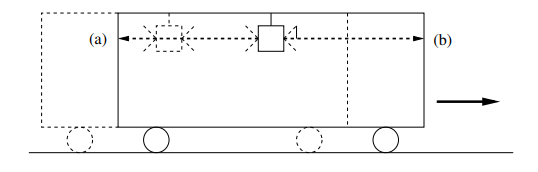
\includegraphics{images/pyt2.png}
    \caption{}
    \label{fig:pyt2}
\end{figure}
Moim zdaniem tak chyba powinno to być - W

Wyobraźmy sobie wagon kolejowy, poruszający się po gładkim, prostym torze ze stałą prędkością (\ref{fig:pyt2}). Dokładnie w środku wagonu zawieszona jest żarówka. Dla obserwatora wewnątrz wagonu, zdarzenie (b) – kiedy światło dociera do przedniej ściany wagonu, i zdarzenie (a), gdy światło dociera do tylnej ściany wagonu zachodzą w tym samym czasie, czyli są równoczesne. Jednak dla obserwatora stojącego na peronie, który obserwuje to samo zjawisko od momentu emisji światła z żarówki, ściany wagonu przemieszczają się, przednia oddala się od promienia światła. Tylna ściana za to przybliża się do promienia wysłanego w jej kierunku i promień ten dotrze do tylnej ściany – (a) przed tym, kiedy drugi promień światła dotrze do przedniej ściany – (b). Dla obserwatora na peronie zdarzenie (a) nastąpi przed zdarzeniem (b). Co więcej, gdyby obok przejeżdżał obserwator pociągiem ekspresowym, który wyprzedzałby nasz wagon, stwierdziłby, że zdarzenie (b) poprzedza zdarzenie (a)!

\noindent \textbf{WZGLĘDNOŚĆ RÓWNOCZESNOŚCI - Dwa zdarzenia równoczesne w jednym układzie inercjalnym nie są na ogół równoczesne w innym.}

\section{Transformacja Lorentza czasu i położenia i jej konsekwencje (skrócenie Lorentza, dylatacja czasu); przykłady wielkości podlegających transformacji Lorentza podobnie jak czas i położenie (czterowektory).}

Tutaj moje (W) notatki z szczególnej teorii względności, gdzie powinno wszystko być: \url{https://drive.google.com/file/d/1uvxyEXb9TcsOzaP0wX-j2wfgkrJ84sSr/view?usp=sharing}

Uczyłam się z mechaniki Taylora (rozdział 15): \url{https://drive.google.com/file/d/1EbQ2YaeomeXPL2FMLMMzpupkQ8cJ4yG9/view?usp=sharing} 

\vspace{0.5cm}
\url{https://www.youtube.com/watch?v=g2xJmc59p-Q}\\

\url{https://www.youtube.com/watch?v=XAW2p0KsdlU&list=PLr6BFY-pH_bmyKF03x3YHDKF7hcks0FVK&index=30}\\

\url{https://www.youtube.com/watch?v=C9GFcBkxP0o&list=PLr6BFY-pH_bmyKF03x3YHDKF7hcks0FVK&index=10&pp=iAQB}\\

\url{https://www.youtube.com/watch?v=wxLMIyp4aq4&list=PLr6BFY-pH_bmyKF03x3YHDKF7hcks0FVK&index=12}\\

\url{https://www.fuw.edu.pl/~jmajewsk/Wyklad-14.pdf}\\


\section{Pęd, energia całkowita i energia wewnętrzna cząstek relatywistycznych.}

Też to jest w notatkach: \url{https://drive.google.com/file/d/1uvxyEXb9TcsOzaP0wX-j2wfgkrJ84sSr/view?usp=sharing}


\noindent Energia podzielona przez $c$ i pęd tworzą czterowektor ($E/c, \textbf{p}$). Wiadomo, że jeśli układ $K'$ porusza się z prędkością $\vec{v} = v \hat{e_x}$ względem układu $K$, to:

\begin{align*}
\frac{E}{c} &= \gamma \biggl(\frac{E'}{c} + \frac{v}{c}p_x'\biggr), \\
p_x &= \gamma \biggl(p_x' + \frac{v}{c} \frac{E'}{c}\biggr), \\
p_y &= p_y', \\
p_z &= p_z'.
\end{align*}

\noindent Energia punktu materialnego o masie $m$ spoczywającego w układzie $K'$ wyrażona względem układu $K$ przybiera postać:
\begin{align*}
\frac{E}{c} &= \gamma \biggl(\frac{E'}{c} + 0 \biggr) = \gamma \frac{E_0}{c}, \\
E &= \gamma E_0.
\end{align*}

\noindent Jeśli $\frac{v}{c} \ll 1$, to:

\begin{align*}
\frac{1}{\sqrt{1 - \frac{v^2}{c^2}}} \approx 1 + \frac{1}{2} \frac{v^2}{c^2}
\end{align*}

\noindent co oznacza, że:

\begin{align*}
E \approx E_0 (1+ \frac{1}{2} \frac{v^2}{c^2}) = E_0 + \frac{1}{2} \frac{E_0}{c^2}v^2,
\end{align*}

\noindent więc:

\begin{align*}
\frac{E_0}{c^2} = m, \:\:\:\: E_0 = mc^2.
\end{align*}

\noindent Energia spoczynkowa ciała o masie $m$ i prędkości $\vec{v} = v \hat{e_x}$ wynosi:

\begin{align*}
E = \frac{mc^2}{\sqrt{1 - \frac{v^2}{c^2}}},
\end{align*}

\noindent natomiast pęd:

\begin{align*}
p_x = \gamma \biggl(0 + \frac{v}{c} \frac{E_0}{c}\biggr) = \gamma m v.
\end{align*}

\noindent Długość czterowektora jest niezmiennikiem transformacji Lorentza, tj. przyjmuje taką samą wartość w każdym inercjalnym układzie odniesienia. Zatem:

\begin{align*}
\frac{E^2}{c^2} - p_x^2 = \frac{E'^2}{c^2} - p_x'^2 &= m^2 c^2, \\
E^2 &= (mc^2)^2 + (p_xc)^2.
\end{align*}

\noindent Całkowita energia ciała wynosi więc:

\begin{align*}
E = \sqrt{m^2c^4 + p_x^2c^2}.
\end{align*}
\section{Zasady zachowania w fizyce.}
W fizyce występują 4 główne zasady zachowania:
\begin{itemize}
\item Zasada zachowania energii -- w układzie izolowanym suma wszystkich rodzajów energii układu jest stała w czasie. Oznacza to, że energia w układzie izolowanym nie może być ani utworzona, ani zniszczona, mogą jedynie zachodzić przemiany z jednych form energii w inne.
\item Zasada zachowania pędu -- suma wektorowa pędów wszystkich elementów układu  izolowanego pozostaje stała. Układ izolowany to taki układ, na który nie działają siły zewnętrzne lub siły te się równoważą. Oddziaływanie między elementami układu siłami wewnętrznymi nie zmienia pędu układu.
\item Zasada zachowania momentu pędu -- dla dowolnego izolowanego układu punktów materialnych całkowita suma ich momentów pędu jest stała. W przypadku bryły sztywnej moment pędu bryły pozostaje stały, gdy nie działa na nią żaden moment siły zewnętrznej.
\item Zasada zachowania ładunku -- w izolowanym układzie ciał całkowity ładunek elektryczny, czyli suma algebraiczna ładunków dodatnich i ujemnych, nie ulega zmianie. Zmiana ładunku układu może zachodzić tylko na drodze przepływu ładunku.
\end{itemize}
\section{Zasady dynamiki Newtona i granice ich stosowalności.}
\url{https://zapytajfizyka.fuw.edu.pl/pytania/jakie-sa-granice-stosowalnosci-zasad-dynamiki-newtona/}\\

\section{Przykłady sił potencjalnych i niepotencjalnych. Prawo powszechnego ciążenia.}
\url{https://zapytajfizyka.fuw.edu.pl/pytania/jakie-sily-sa-potencjalne-lub-zachowawcze/}
\subsection{Siły potencjalne}
\textbf{Siłami potencjalnymi} nazywa się w ogólności siły, dla których istnieje funkcja skalarna (zwana potencjałem, która każdemu punktowi przestrzeni i czasie przypisuje wartość $V$), taka że jej gradient jest równy danej sile. Okazuje się, że oprócz sił potencjalnych niezależnych od czasu istnieją siły potencjalne \textit{zależne od czasu}:
\begin{equation*}
    \vec F(\vec r,t) = -\text{grad}\,\,V(\vec r,t).
\end{equation*}
Gdy potencjał nie jest zależny od czasy mamy do czynienia z \textbf{siłami zachowawczymi}:
\begin{equation*}
    \vec F(\vec r) = -\text{grad}\,\,V(\vec r)
\end{equation*}
Wówczas suma energii potencjalnej i kinetycznej jest niezależną od czasu energią mechaniczną:
\begin{equation*}
    E=T(\vec r)+V(\vec r)
\end{equation*}

Praca w polu sił zachowawczych nie zależy od toru, po jakim przemieszcza się ciało, a jedynie od różnicy energii potencjalnej:
\begin{equation*}
    W_{\vec r_A\to \vec r_B} = V(\vec r_B)-V(\vec r_A)
\end{equation*}
co oznacza, że praca ta jest równa różnicy energii potencjalnych między punktem końcowym a początkowym.

Siłami zachowawczymi są wszystkie siły centralne. Np. siłami centralnymi są siły grawitacyjne w klasycznej teorii grawitacji Newtona, siły kulombowskie oddziaływań między ciałami posiadającymi ładunki elektryczne. Także siły sprężystości ciał doskonale sprężystych są siłami centralnymi.

Niektórzy przyjmują, że wszystkie siły zachowawcze są potencjalne (ale niektórzy, że np. siła Lorentza jest zachowawcza, ale nie jest potencjalna).

Nie każda siła potencjalna będzie zachowawcza. Np. siła, która działa na cząstkę naładowaną w zmiennym polu elektrycznym:
\begin{equation*}
    \vec F_E(\vec r,t) = q \vec E_0 \cos(\omega t)
\end{equation*}

Potencjał w tym przypadku jest zależny od czasu:
\begin{equation*}
    V(\vec r,t)= -\int_0^z \vec F_E(\vec r,t) d\vec r
= -q E_0 z\, \sin\, \omega t
\end{equation*}

Ale nie jest to siła zachowawcza, bo pochodna potencjału po czasie się nie zeruje, czyli cząstka w takim polu zmienia swoją energię:
\begin{equation*}
    \frac{\partial{V}(\vec r,t)}{\partial t}
= qE_0 z \cos\omega t \ne 0
\end{equation*}

\subsection{Siły niepotencjalne}
Siły niepotencjalne to np. siły oporu, tarcia, itp. Zależą one od prędkości poruszającego się obiektu i nie można ich opisać przy pomocy potencjału.

\textbf{Potencjał} to wielkość charakteryzująca stan pola elektrycznego, magnetycznego lub grawitacyjnego w danym punkcie.

\subsection{Prawo powszechnego ciążenia}
Prawo powszechnego ciążenia głosi, że siła przyciągania grawitacyjnego między dwoma ciałami jest proporcjonalna do iloczynu ich mas i odwrotnie proporcjonalna do kwadratu odległości.

Matematycznie związek ten wyraża się wzorem:
\begin{equation*}
    \boldsymbol F = G \frac{m_1 m_2}{r^2} \boldsymbol e
\end{equation*}
gdzie:\\
$G$ -- stała grawitacji,\\
$m_1$ -- masa pierwszego ciała,\\
$m_2$ -- masa drugiego ciała,\\
$r$ -- długość wektora łączącego środki obu ciał,\\
$\boldsymbol e=\frac{\boldsymbol r}{r}$ -- wersor (wektor jednostkowy) $(|\boldsymbol e| =1)$ osi łączącej środki mas obu ciał.

Siła ta działa na linii łączącej środki mas ciał i występuje pomiędzy wszystkimi obiektami we Wszechświecie.

Siła $\boldsymbol F$ jest wektorem, a jej wartość (długość tego wektora $F=\frac{\boldsymbol F} {|\boldsymbol e|}$) jest równa:
\begin{equation*}
    F = G \frac{m_1 m_2}{r^2}.
\end{equation*}


\section{Zagadnienie dwóch ciał i problem Keplera (środek masy i zasada zachowania momentu pędu).}
2021-MiSTW-wyklad-16-21 \\
\url{https://www.fuw.edu.pl/~szymacha/pfw19.pdf} \\
\url{https://www.kk.us.edu.pl/mechteor/bw8_dwaciala.pdf}
\section{Moment bezwładności i zasady dynamiki ruchu bryły sztywnej.}
\url{http://www.ftj.agh.edu.pl/~wierzbanowski/R_obr(3).pdf}\\
\url{https://fais.uj.edu.pl/documents/41628/142476873/PF11-Dynamika_bryly_sztywnej.pdf/53243967-fa6a-4019-a569-ad80a75d6c6a}
\begin{figure}[H]
    \centering
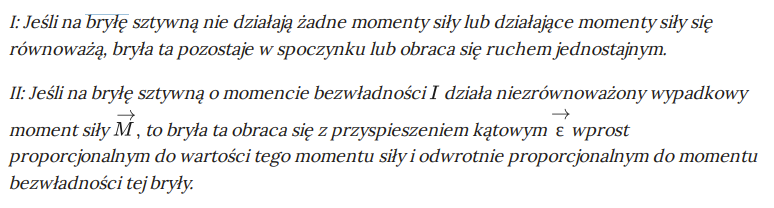
\includegraphics[width=0.9\textwidth]{images/sztywna1.png}
\end{figure}
\begin{figure}[H]
    \centering
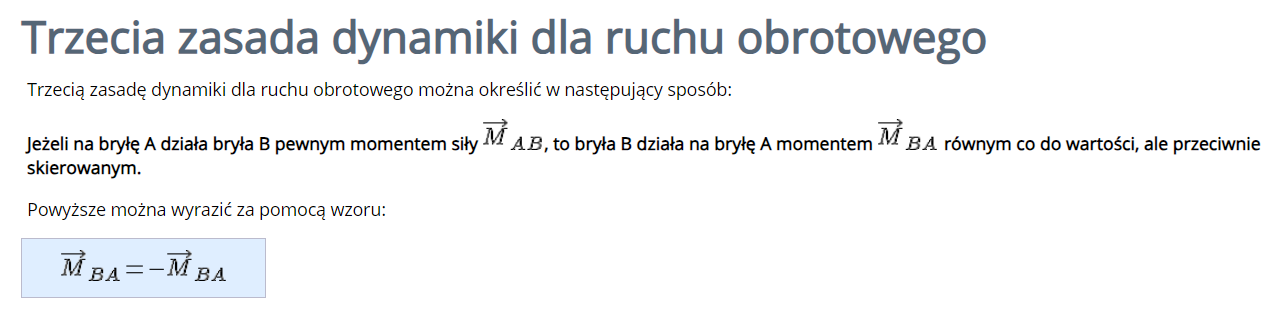
\includegraphics[width=0.9\textwidth]{images/stywna2.png}
\end{figure}


\section{Prawo Coulomba, prawo Gaussa, potencjał pola elektrycznego.}
\subsection{Prawo Coulomba}
Siła jaką spoczywający ładunek $q$ działa na ładunek próbny $Q$ znajdujący się w odległości $R$ dana jest prawem Coulomba:
\begin{equation*}
    F = \frac{1}{4\pi \epsilon_0}\frac{qQ}{R^2}\hat{R},
\end{equation*}
gdzie $\epsilon_0=8,85\cdot 10^{-12}\frac{C^2}{N\cdot m^2}$ to przenikalność elektryczna próżni. \\
Prawo Coulomba głosi, że siła jest wprost proporcjonalna do iloczynu ładunków i odwrotnie proporcjonalna do kwadratu odległości między nimi. $R$ jest wektorem reprezentującym różnicę położeń ładunków $q$ (wektor $r'$) i $Q$ (wektor $r$): $R=r-r'$. $R$ jest jego długością, a $\hat{R}$ wersorem wskazującym jego kierunek i zwrot. Siła jest skierowana wzdłuż linii łączącej $q$ z $Q$; jest odpychająca, kiedy $q$ i $Q$ są tego samego znaku, i przyciągająca, jeśli ich znaki są przeciwne. \\

Jeśli mamy kilka ładunków punktowych $q_{1,2,...,n}$, których odległości od ładunku $Q$ wynoszą odpowiednio $R_{1,2,...,n}$, to całkowita siła działająca na $Q$ jest dana wzorem:
\begin{equation*}
    F=F_1+F_2+...=\frac{1}{4\pi\epsilon_0}\left( \frac{q_1}{R_1^2}\hat{R_1}+\frac{q_2}{R_2^2}\hat{R_2}+... \right)Q;
\end{equation*}
lub inaczej:
\begin{equation*}
    F=QE, \; E(r) = \frac{1}{4\pi\epsilon_0} \sum_{i=1}^{n} \frac{q_i}{R_i^2}\hat{R_i}.  
\end{equation*}

$E$ nazywa się natężeniem pola elektrycznego ładunków-źródeł. Jest ono funkcją położenia $r$ - ponieważ wektory $R_i$ zależą od punktu, w którym mierzymy pole - ale nie zależy od wielkości ładunku próbnego $Q$. Natężenie pola elektrycznego to zależna od położenia wielkość wektorowa, która jest określona przez rozmieszczenie ładunków-źródeł; $E(r)$ można interpretować fizycznie jako siłę na jednostkę ładunku, jaka działa na ładunek próbny umieszczony w określonym punkcie. \\

Jeśli ładunek jest rozłożony w sposób ciągły wzdłuż krzywej, a jego gęstość liniowa wynosi $\lambda$, to $dq = \lambda dl'$ (gdzie $dl'$ jest infinitezymalnym przyrostem długości
wzdłuż krzywej); jeśli ładunek rozłożony jest w sposób ciągły na pewnej powierzchni, a jego gęstość powierzchniowa wynosi $\sigma$, to $dq = \sigma da'$ (gdzie $da'$ jest infinitezymalnym elementem powierzchni): jeśli ładunek rozłożony jest w sposób ciągły w pewnej objętości, a jego gęstość objętościowa wynosi $\rho$, to $d\rho = \rho d\tau'$ (gdzie $d\tau'$ jest infinitezymalnym elementem objętości).
\begin{equation*}
    E(r) = \frac{1}{4\pi\epsilon_0}\int \frac{1}{R^2}\hat{R}dq
\end{equation*}

\textit{Podstawy elektrodynamiki - Griffiths, str. 80}

\subsection{Prawo Gaussa}
\textit{Podstawy elektrodynamiki - Griffiths, str. 89}

\subsection{Potencjał pola elektrycznego}
\textit{Podstawy elektrodynamiki - Griffiths, str. 100}

\section{Prąd elektryczny, prawo Ohma, rozkład prądu i pola elektrycznego w przewodniku, zasada zachowania ładunku elektrycznego. Równanie ciągłości dla prądu}

Natężeniem prądu płynącego przez przewodnik nazywany ładunek przepływający w jednostkowym czasie przez dany przekrój przewodnika. Ładunek liniowy o gęstości $\lambda$ poruszający się z prędkością $v$ daje prąd o natężeniu: $I=\lambda v$. Siła magnetyczna działająca na odcinek przewodnika z prądem jest równa:
\begin{equation*}
    F_{mag}=\int (v \times B)dq = \int (v\times B) \lambda dl = \int (I\times B) dl.
\end{equation*}

\subsection{Prawo Ohma}
Ażeby mógł płynąć prąd elektryczny, na ładunku musi działać siła. Prędkość ruchu ładunków jako odpowiedź na działającą siłę zależy od rodzaju materiału, w którym płynie prąd. Dla większości substancji gęstość prądu $J$ jest proporcjonalna do siły $f$ działającej na jednostkowy ładunek: $J=\sigma f$. \\
Współczynnik proporcjonalności $\sigma$ jest stałą empiryczną zależną od materiału z którego wykonany jest półprzewodnik; nosi on nazwę przewodności elektrycznej właściwej substancji. Jego odwrotnością jest opór elektryczny właściwy $\rho=1/\sigma$. Siła powodująca ruch ładunków może mieć dowolną naturę. Zwykle jest to siła elektromagnetyczna, wtedy: 
\begin{equation*}
    J=\sigma E.
\end{equation*}
Całkowite natężenie prądu płynącego od jednej elektrody do drugiej jest proporcjonalne do różnicy potencjałów pomiędzy elektrodami:
\begin{equation*}
    V=IR
\end{equation*}

\subsection{Rozkład prądu i pola elektrycznego w przewodniku}
\textit{Podstawy elektrodynamiki - Griffiths, str. 120}

\subsection{Zasada zachowania}

Ładunek jest zachowany; nie można go wytworzyć ani zniszczyć - zawsze było tyle ładunku, co teraz. Jest to tak zwane prawo globalnego zachowania ładunku. Lokalna zasada zachowania ładunku mówi, że jeśli całkowity ładunek zawarty w jakiejś objętości zmienia się o pewną wartość, to dokładnie taka sama ilość ładunku musi przepłynąć przez powierzchnię ograniczającą tę objętość. Ładunek zawarty w obszarze $V$ możemy zapisać jako:
\begin{equation*}
    Q(t) = \int_V \rho(r,t) d\tau,
\end{equation*}
natomiast prąd płynący przez brzeg tego obszaru $S$ jest równy $\int_S J\cdot da$, tak więc zasada zachowania ładunku mówi, że:
\begin{equation*}
    \frac{dQ}{dt} = -\int_S J \cdot da.
\end{equation*}
Wykorzystując równanie na $Q(t)$ po lewej stronie, a po prawej twierdzenie Gaussa, otrzymujemy:
\begin{equation*}
    \int_V \frac{\partial \rho}{\partial t} d\tau = --\int_V \nabla \cdot J d\tau. 
\end{equation*}
Ponieważ jest to prawda dla dowolnego obszaru, można zapisać:
\begin{equation*}
    \frac{\partial \rho}{\partial t} = - \nabla \cdot J . 
\end{equation*}
\textit{Podstawy elektrodynamiki - Griffiths, str. 377}

\subsection{Równanie ciągłości}

Natężenie prądu płynącego przez powierzchnię $S$ można zapisać jako:
\begin{equation*}
    I = \int_{S} J\cdot da.
\end{equation*}
Całkowity ładunek wypływający w jednostce czasu w obszaru $V$ jest równy:
\begin{equation*}
    \oint_S J\cdot da = \int_V (\nabla \cdot J) d\tau.
\end{equation*}
Ponieważ całkowity ładunek jest zachowany, cokolwiek wpływa przez powierzchnię, musi pomniejszać ładunek pozostały w środku:
\begin{equation*}
    \int_V (\nabla \cdot J) d\tau=-\frac{d}{dt} \int_V \rho d\tau = -\int_V \left( \frac{\partial \rho}{\partial t}\right)dz.
\end{equation*}
Znak minus odzwierciedla fakt, że wpływ ładunku zmniejsza ładunek pozostający w objętości $V$. Równość ta jest prawdziwa dla dowolnej objętości, co oznacza, że:
\begin{equation*}
    \nabla \cdot J = \frac{\partial \rho}{\partial t}.
\end{equation*}
Jest to dokładne matematyczne sformułowanie lokalnej zasady zachowania ładunku. Jest ono nazywane równaniem ciągłości. \\
Kiedy prąd stały płynie przez przewodnik, jego natężenie $I$ musi być stałe wzdłuż całego przewodnika; w przeciwnym wypadku ładunek musiałby się gdzieś zbierać i, w konsekwencji, nie byłby to prąd stały. Ten sam argument mówi, że w magnetostatyce $\partial \rho / \partial t=0$, a zatem równanie ciągłości przybiera postać:
\begin{equation*}
    \nabla \cdot J = 0.
\end{equation*}
\textit{Podstawy elektrodynamiki - Griffiths, str. 242}

Równanie ciągłości: \url{https://encyklopedia.pwn.pl/haslo/rownanie-ciaglosci;3886409.html}
\section{Pole magnetyczne prądu stałego}

Z równań Maxwella wynika, że  pole magnetyczne jest efektem ruchu ładunków elektrycznych lub zmiennego pola elektrycznego. Źródłem pola magnetycznego będzie więc prąd elektryczny. Dla prądu o stałym natężeniu, powstaje stałe, statyczne, pole magnetyczne. 

Pole magnetyczne liniowego prądu stałego jest określane przez prawo Biota-Savarta. Prawo to pozwala nam na określenie w dowolnym punkcie przestrzeni indukcji pola magnetycznego, której źródłem jest element przewodnika, przez który płynie prąd elektryczny:
\begin{equation*}
    B(r) = \frac{\mu_0}{4\pi}\int \frac{I\times \hat{R}}{R^2}dl' = \frac{\mu_0}{4\pi}l\int\frac{dI'\times \hat{R}}{R^2}.
\end{equation*}
Całka liczona jest wzdłuż całej drogi prądu w kierunku jego przepływu; $dl'$ jest elementem długości przewodnika, a $R$ jest wektorem skierowanym od źródła do punktu $r$. Stała $\mu_0=4\pi \cdot 10^{-7}\; \mathrm{N/A^2}$ nazywana jest przenikalnością magnetyczną próżni. Indukcja magnetyczna jest mierzona w $\mathrm{N/(A\cdot m)}$, czyli w teslach. 

\begin{figure}[H]
    \centering
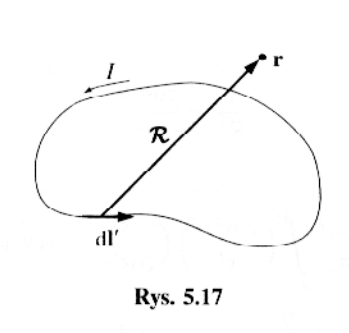
\includegraphics[width=0.3\textwidth]{images/biot.png}
\end{figure}

Prawo Biota-Savarta daje nam związek między wkładem do pola magnetycznego pochodzącego od przepływu prądu w określonym miejscu i w zależności od tego jak odległe jest miejsce przepływu prądu od miejsca, w którym obliczamy pole magnetyczne.

Dla prądów powierzchniowych i objętościowych prawo Biota-Savarta przybiera postać:
\begin{equation*}
    B(r) = \frac{\mu_0}{4\pi}\int \frac{K(r')\times \hat{R}}{R^2}da', \; B(r) = \frac{\mu_0}{4\pi}\int \frac{J(r')\times \hat{R}}{R^2}d\tau'
\end{equation*}

\section{Siła Lorentza i ruch cząstek naładowanych w polach elektrycznym i magnetycznym.}

Siła działająca na ładunek $Q$ poruszający się z prędkością $v$ w polu o indukcji magnetycznej $B$ jest dana wzorem:
\begin{equation*}
    F_{mag}=Q(v\times B).
\end{equation*}
Nosi ona nazwę siły Lorentza. W obecności obu pól, elektrycznego i magnetycznego, siła wypadkowa działająca na ładunek $Q$ jest równa:
\begin{equation*}
    F=Q(E+(v\times B)).
\end{equation*} 
Siły magnetyczne nie wykonują pracy. Jeśli ładunek $Q$ przesunie się o $dI=vdt$, to wykonana praca równa jest:
\begin{equation*}
    dW_{mag}=F_{mag}\cdot dI=Q(v\times B)\cdot vdt=0.
\end{equation*}
Jest tak dlatego, że $v\times B$ jest wektorem prostopadłym do $v$, a zatem $(v\times B)\cdot v=0$. Siły magnetyczne mogą zmienić kierunek ruchu cząstki, nie mogą jednak zmienić wartości jej prędkości.  (str. 230)

\section{Prawo indukcji Faradaya i reguła Lenza - 333}
\url{https://home.agh.edu.pl/~kakol/efizyka/w24/main24b.html} \\

Zmiana pola magnetycznego indukuje pole elektryczne. Jeśli siła elektromotoryczna $\epsilon$ jest równa szybkości zmiany strumienia
\begin{equation*}
    \epsilon = \oint E\cdot dl = - \frac{d\Phi}{dt},
\end{equation*}
to natężenie pola elektrycznego E wiąże się ze zmianą indukcji magnetycznej B równaniem
\begin{equation*}
    \oint E\cdot dl = - \int \frac{\partial B}{\partial t}\cdot da.
\end{equation*}
Jest to całkowita postać prawa Faradaya. Posługując się twierdzeniem Stokesa, znajdziemy jego postać różniczkową:
\begin{equation*}
    \nabla \times E = \frac{\partial B}{\partial t}.
\end{equation*}
W przypadku pola statycznego (B=const.) prawo Faradaya redukuje się do starego prawa $\oint E\cdot dl=0$ (lub $\nabla \times E=0$. \\
UNIWERSALNA REGUŁA STRUMIENIA: Jeśli zmienia się strumień magnetyczny przenikający przez obwód, w obwodzie indukuje się SEM:
\begin{equation*}
    \epsilon = -\frac{d\Phi}{dt}
\end{equation*}

\textbf{Reguła Lenza} pomaga w poprawnym określeniu kierunku prądu: Natura nie znosi zmiany strumienia. \\
Indukowany prąd będzie płynął w takim kierunku, że dodatkowy strumień powstały w wyniku jego przepływu sprzeciwia się zmianie pierwotnego strumienia. (336)

\section{Pełny układ równań Maxwella z warunkami brzegowymi na granicy ośrodków. - 359}

\begin{gather*}
    1. \; \nabla \cdot E = \frac{1}{\epsilon_0}\rho \\
    2. \; \nabla \cdot B = 0 \\
    3. \; \nabla \times E = - \frac{\partial B}{\partial t} \\
    4. \nabla \times B = \mu_0 J + \mu_0\epsilon_0\frac{\partial E}{\partial t}
\end{gather*}
Część warunków brzegowych: \url{https://www.youtube.com/watch?v=zmb0ZuwAa2Y}

Wszystkie warunki brzegowe w Griffitsie (strona 364)
\section{Ruch okresowy (parametry); rozkład na drgania proste.}
Analiza Fouriera: \url{https://www.if.pw.edu.pl/~anadam/WykLadyFO/FoWWW_13a.html}
\section{Oscylator harmoniczny: drgania swobodne, tłumione i wymuszone oraz zjawisko rezonansu.}
\url{https://home.agh.edu.pl/~kakol/efizyka/w12/main12e.html}
\section{Zjawisko Dopplera.}
\url{https://home.agh.edu.pl/~kakol/efizyka/w13/main13h.html}
Polecam tą Panią: \url{https://www.youtube.com/watch?v=u5mTsUHPKKc}
\section{Fale elektromagnetyczne. Prawa odbicia i załamania fal elektromagnetycznych; współczynnik odbicia, polaryzacja fali odbitej i załamanej (kąt Brewstera).}

W artykule opisana jest polaryzacja fali odbitej pod kątem Brewstera: \url{file:///C:/Users/wikto/Downloads/A_New_Optoelectronic_Switch_The_Dielectric_of_a_Ca.pdf}
\section{Spójność, dyfrakcja i interferencja fal: dyfrakcja na pojedynczej szczelinie, doświadczenie Younga, siatka dyfrakcyjna.}

\url{https://www.igf.fuw.edu.pl/m/courses_materials/05/ca/05ca10ab-9cb3-47eb-b329-30d39e42e24a/MNO_Wyk_VI_Optyka_InterferOMETRY_KOHERENCJA_30_11_2020.pdf} \\
\url{https://openstax.org/books/fizyka-dla-szk%C3%B3%C5%82-wy%C5%BCszych-tom-3/pages/4-1-dyfrakcja-na-pojedynczej-szczelinie}

\url{https://www.uj.edu.pl/c/document_library/get_file?uuid=5c6a0292-96d9-43c6-a573-d96397d015a2&groupId=5046939}

\section{Równowaga termiczna i temperatura; skale temperatury. Ciepło, procesy wymiany ciepła.}

\subsection{Równowaga termiczna}
\begin{enumerate}
    \item Gdy zetkniemy dwa ciała o różnej energii wewnętrznej, następuje przepływ energii, który prowadzi do wyrównania wielkości, którą nazwaliśmy temperaturą. Mówimy, że ciała w kontakcie, dla których wyrównaniu uległa temperatura, pozostają w równowadze termicznej. 
    \item Przepływ energii zachodzi od ciała o wyższej temperaturze do ciała o niższej,
    \item Jeśli układy A i B mogące wymieniać ze sobą energię wewnętrzną, są ze sobą w równowadze termicznej, i to samo jest prawdą dla układów B i C, to układy A i C są również ze sobą w równowadze termicznej. (Zerowa zasada TD)
    \item Ciało w równowadze termicznej ma wszędzie tę samą temperaturę. 
\end{enumerate}

\subsection{Ciepło}
Ciepło definiujemy jako wzajemne oddziaływanie dwóch ciał o różnej temperaturze - wywołujące przemianę, w której przekazywanie energii prowadzi tylko do zmiany energii wewnętrznych tych ciał, przy założeniu:
\begin{enumerate}
    \item braku oddziaływania otoczenia na układ (np. elektrycznego lub magnetycznego);
    \item niewystępowania reakcji chemicznych;
    \item istnienia sztywnych ograniczeń dla obu rozpatrywanych ciał, uniemożliwiających zmianę kształtu i objętości substancji.
\end{enumerate}
Zasób przetransportowanej w ten sposób energii od jednego do drugiego ciała nazywamy ciepłem. Pojęcie ciepła jest ściśle związane z zachodzeniem przemiany TD i gdy przemiana nie zachodzi, nie ma transportu ciepła, co jest równoznaczne z nieistnieniem ciepła. Ciepło zależy nie tylko od stanu początkowego i końcowego substancji, ale również od drogi przemiany, a zatem ciepło nie jest parametrem stanu.\\
Ciepło elementarne nie $\delta Q$ nie jest różniczką zupełną parametrów stanu, a oznacza jedynie elementarny przyrost ciepła wymienionego między układem a otoczeniem. Ciepło przemiany między stanem początkowym i końcowym wyraża się wzorem:
\begin{equation*}
    Q_k - Q_p = \Delta Q = \int_{Q_p}^{Q_k}\delta Q.
\end{equation*}
Wynik całkowania jest dodatni $\Delta Q>0$, gdy ciepło jest doprowadzanie do układu, a ujemny $\Delta Q<0$ gdy ciepło jest odprowadzane z układu. \\

Można wymienić trzy mechanizmy odpowiedzialne za przepływ ciepła:
\begin{enumerate} 
    \item Przewodnictwo cieplne jest wymianą ciepła między materią, która się nie porusza, poprzez fizyczny kontakt (stykanie się dwóch materiałów ze sobą; stacjonarność materii jest tylko makroskopowa, wiadomo bowiem, że ruchy cieplne atomów i cząsteczek występują w każdej temperaturze powyżej zera bezwzględnego). To przewodnictwo cieplne odpowiedzialne jest za wymianę ciepła z palnika na piecu przez dno patelni do jedzenia znajdującego się na niej.
    \item Konwekcja jest wymianą ciepła przez makroskopowy ruch płynu. Taki rodzaj przepływu ciepła występuje na przykład w piecu z wymuszonym obiegiem powietrza lub w globalnych układach pogodowych.
    \item Wymiana ciepła przez promieniowanie pojawia się wtedy, kiedy np. mikrofale, promieniowanie podczerwone, światło widzialne lub inny rodzaj promieniowania elektromagnetycznego jest wysyłany (emitowany) lub pochłaniany (absorbowany) przez ciało. Oczywistym przykładem jest ogrzewanie Ziemi przez Słońce, mniej oczywistym – promieniowanie cieplne wysyłane przez ludzkie ciało.
\end{enumerate}

\subsection{Skale temperatury}
Ważną rolę przy ustalaniu skali temperatury odgrywa istnienie punktów stałych temperatury. Procesy zachodzące w stałej temperaturze (przemiany fazowe) mogą służyć za podstawę wyznaczenia charakterystycznych punktów temperatury. Można wybrać jeden taki punkt (funkcja postaci $T=Ax$), dwa (funkcja liniowa), trzy (funkcja kwadratowa) lub więcej. Fahrenheit wybrał 2 punkty termometryczne: 0\degree F jako temperaturę mieszaniny wody i lodu z solą oraz 32\degree F jako temperaturę mieszaniny wody i lodu. W skali Celsjusza wybrano punkt 0\degree C (punkt topnienia lodu) i 100\degree C (punkt wrzenia wody). Wzory przeliczające te dwie skali:
\begin{equation*}
    T_F = T_C\cdot 1,8 + 32; \
    T_C = (T_F-32)/1,8
\end{equation*}
Uznano, że znacznie lepszym punktem temperaturowym od zamrażania wody jest punkt potrójny wody, bo występuje w ściśle ustalonej temperaturze i ciśnieniu. W skali Kelwina przyjęto T=273,16 K za dokładną wartość dla punktu potrójnego wody. 

\section{Promieniowanie cieplne ciał: współczynniki absorpcji i emisji promieniowania, ciało doskonale czarne, prawo przesunięć Wiena, prawo Stefana-Boltzmanna.}

\url{http://www.ftj.agh.edu.pl/~Wolny/index2.php.htm}

\section{Druga zasada termodynamiki i pojęcie entropii.}

ENTROPIA S - liczba mikrostanów w przypadku układów, gdzie molekuł jest bardzo dużo, jest mało wygodne, dlatego zamiast operować wielkością $\Omega$, definiuje się wielkość nazywaną entropią: $S=k\cdot ln\Omega$.\\
Druga zasada TD stwierdza, że wszystkie zjawiska zachodzące samorzutnie w przyrodzie, są zjawiskami nieodwracalnymi. Gdy układ zamknięty o temperaturze T, jednakowej w każdym jego punkcie, wymienia z otoczeniem w procesie odwracalnym ciepło $dQ$, wówczas entropia tego układu zmienia sie o wartość $dS$ równą: $dS = \frac{dQ}{T}$. W dowolnym procesie samorzutnym spełniona jest dla rozpatrywanego układu równość: $dS - dQ/t \geq 0$, przy czym znak równości odnosi się do procesów odwracalnych, znak nierówności - do procesów nieodwracalnych samorzutnych. Entropia pozwala określić czy dany stan jest osiągalny w procesie samorzutnym. 

\section{Równowaga termodynamiczna.}

Równowaga termodynamiczna – pojęcie stosowane w termodynamice. Oznacza stan, w którym makroskopowe parametry układu, takie jak ciśnienie, objętość i wszystkie funkcje stanu, są stałe w czasie.

Aby zachodziła równowaga termodynamiczna, muszą zachodzić trzy równowagi:
\begin{itemize}
    \item \textbf{równowaga chemiczna} -- brak makroskopowego przepływu cząstek i brak reakcji chemicznych
    \item \textbf{równowaga mechaniczna} -- wszystkie punkty pozostają w spoczynku i nie występują niezrównoważone siły
    \item \textbf{równowaga termiczna} -- brak przepływu energii (ciepła)
\end{itemize}

Tak znalazłam na internecie, ale wydaje mi się, że np. reakcje mogą zachodzić, tylko muszą się ze sobą równoważyć.

Układ jest w równowadze termodynamicznej, jeżeli nie zachodzą w nim żadne systematyczne zmiany opisujących go parametrów i nie występują zjawiska transportu. Podstawową cechą wszystkich układów izolowanych jest dążenie do stanu równowagi termodynamicznej. 

\section{Równanie stanu gazu doskonałego, przemiany gazowe, molowe ciepła właściwe gazów.}
\url{http://cmf.p.lodz.pl/iowczarek/materialy/termodynamika/przemiany.html} -- ten link niestety nie działa.

Gazem doskonałym nazywamy gaz spełniający równanie stanu Clapeyrona:
\begin{equation*}
    pV=nRT
\end{equation*}
Właściwości gazu doskonałego:
\begin{enumerate}
    \item objętość cząsteczek jest znikoma w stosunku do objętości gazu;
    \item cząsteczki gazu mają rozmiar punktów materialnych;
    \item cząsteczki gazu wykazują cechy doskonale sprężystych kulek znajdujących się w ciągłym przypadkowym chaotycznym ruchu, powodującym zderzenia cząsteczek między sobą oraz ze ściankami naczynia, w którym są zawarte;
    \item między cząsteczkami nie występują żadne inne oddziaływania poza zderzeniami doskonale sprężystymi;
    \item bezpośrednią miarą temperatury gazu jest średnia energia kinetyczna jego cząsteczek.
\end{enumerate}

Przemiany gazowe: \url{https://drive.google.com/file/d/1tv0qibZHEfI6AiKuU7wj6J_jLmSBNPAm/view?usp=sharing}

\begin{figure}[H]
    \centering
    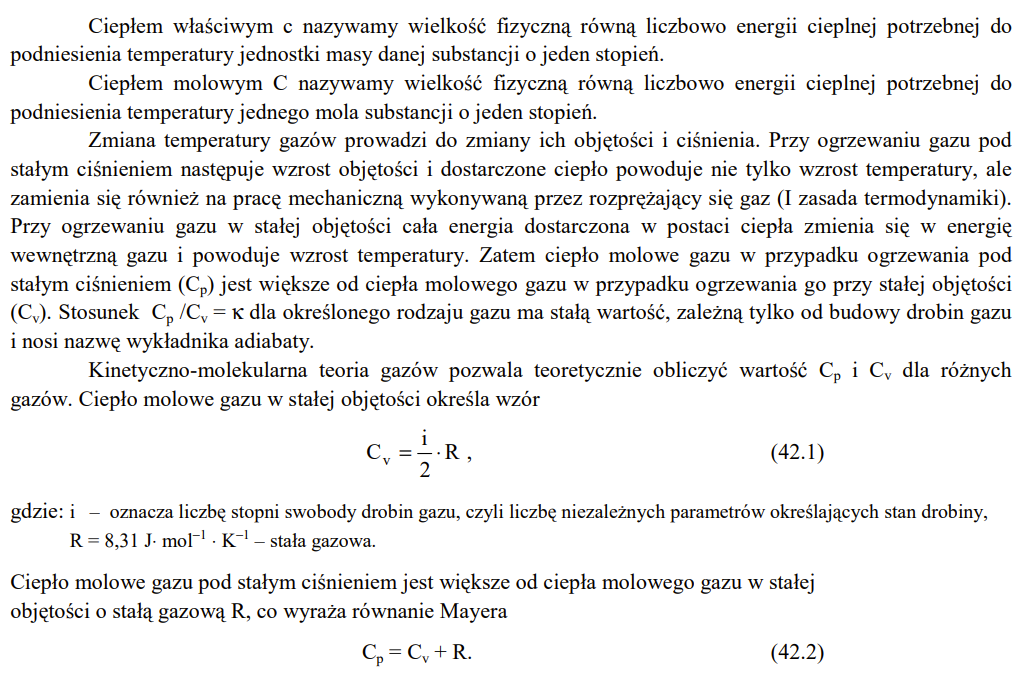
\includegraphics[width=0.8\textwidth]{images/ciepło właściwe.png}
\end{figure}

\begin{equation*}
    C_p=C_v+nR
\end{equation*}
 


\section{Przemiany fazowe I rodzaju (przykłady) i współistnienie faz; przemiany fazowe drugiego rodzaju.}

\url{https://www.if.pw.edu.pl/~anadam/WykLadyFO/FoWWW_24.html}

Przemiany fazowe są szczególnego rodzaju procesami termodynamicznymi, w których zmiana stanu układu jest połączona ze zmianą fazy substancji tworzącej ten układ. Przemiana fazowa I-go rodzaju zachodzi wtedy, gdy w tym procesie obserwuje się:
\begin{enumerate}
    \item Niezerowe ukryte ciepło (entalpia) przemiany;
    \item Występowanie nukleacji (zarodnikowania nowej fazy), czyli że przemiana nie zachodzi w całej objętości jednocześnie;
    \item Istnienie zjawisk “prze” (przechłodzenia i przegrzania).
\end{enumerate}

Najlepiej znanymi przykłada przemian fazowych I-go rodzaju są powszechnie znane zmiany stanu skupienia : parowanie, skraplanie, topnienie, krystalizacja. Zjawiska przemian fazowych są rezultatem powszechnej w przyrodzie tendencji każdego układu do osiągnięcia stanu, w którym energia tego układu jest najmniejsza. Wygodnym do analizy przemian fazowych rodzajem energii jest tzw. energia swobodna F = U - TS, czyli energia, która w całości może zostać zamieniona na pracę. Entropia S zostanie omówiona później w kontekście II. zasady termodynamiki. \\

Wykresy energii F w funkcji temperatury dla dwóch stanów układu A i B są przedstawione czarnymi liniami. W niższej temperaturze stabilny – wygodniejszy energetycznie - jest stan A (ma niższe F), a w wyższej stabilny jest B (teraz on ma niższe F). W czasie ogrzewania układ przesuwa się po czerwonej linii. W temperaturze T0 zachodzi przemiana fazowa ze stanu A do B. W tym punkcie energie swobodne obu faz są jednakowe: FA = FB. W całym procesie ogrzewania układ przyjmuje najniższą dopuszczalną dla niego wartość energii swobodnej.
\begin{figure}[H]
    \centering
    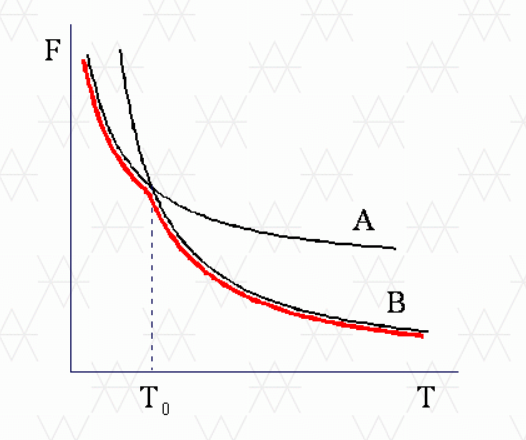
\includegraphics[width=0.5\textwidth]{przemiany.png}
    \caption{Caption}
    \label{fig:26}
\end{figure}
 

Fazy, jakie może przyjmować układ, wygodnie jest przedstawiać na diagramach fazowych w układzie temperatura – ciśnienie p-T. \\

W przemianie fazowej II-go rodzaju NIE obserwuje się:
\begin{enumerate}
    \item Niezerowego ukrytego ciepła (entalpii) przemiany;
    \item Nukleacji (zarodnikowania nowej fazy), czyli że przemiana zachodzi w całej objętości jednocześnie;
    \item Zjawisk “prze” (przechłodzenia i przegrzania).
\end{enumerate}
W temperaturze, w której zachodzi przemiana fazowa II. rodzaju  nie ma zmiany stanu skupienia, a występuje tylko zmiana symetrii układu. Przykładami przemian fazowych II-go rodzaju są: przemiana ferromagnetyk - paramagnetyk (bardzo gorący gwóźdź stalowy nie jest przyciągany przez magnes), przemiana przewodnik - nadprzewodnik (Prąd elektryczny raz wzbudzony w pierścieniu nadprzewodzącym będzie w nim płynął praktycznie bez końca. O płynącym prądzie świadczy wytwarzane przez niego pole magnetyczne B. Pole magnetyczne nie wnika w nadprzewodnik, co powoduje lewitację nad nim magnesu (efekt Meissnera))

 
\section{Gazy rzeczywiste i ciecze: para nasycona, parowanie i wrzenie.}
\url{https://dydaktyka.fizyka.umk.pl/fizykaAiR/gas_phase.pdf}\\
\url{http://pracownicy.uwm.edu.pl/wojsob/pliki/dydaktyka/td-09.pdf}

\begin{figure}[H]
    \centering
    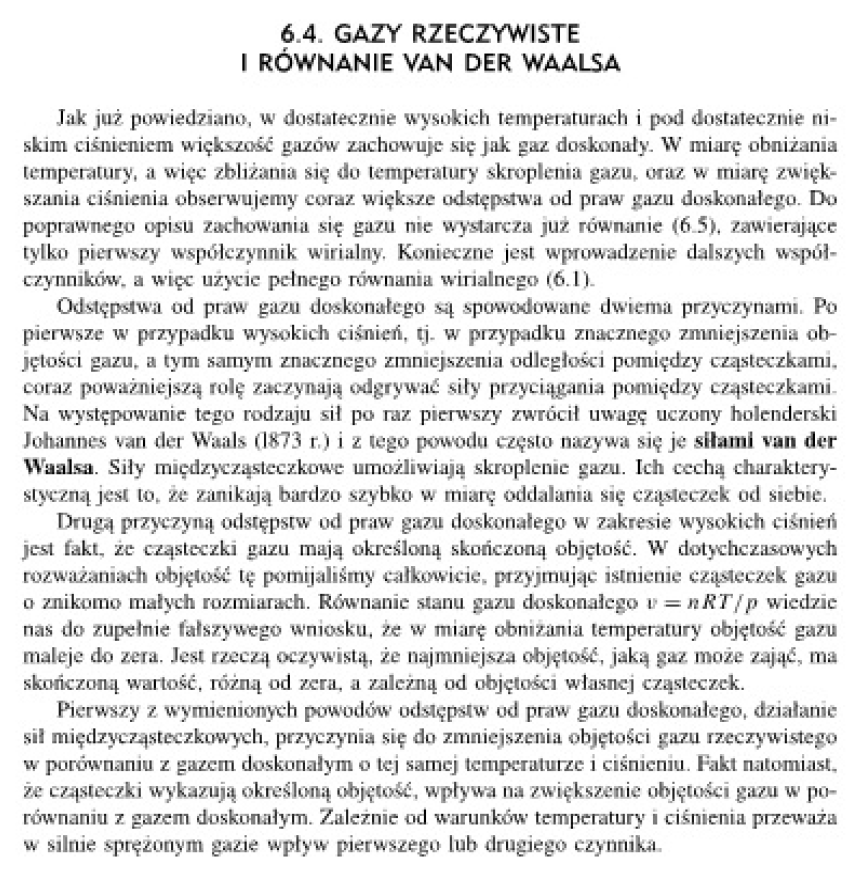
\includegraphics[width=0.8\textwidth]{images/rzeczywiste.png}
\end{figure}

\section{Trzecia zasada termodynamiki i nieosiągalność zera bezwzględnego. - 292}

Trzecia zasada TD głosi: \\
Zasób energii każdego układu złożonego z substancji czystej w stanie kryształu doskonałego w temperaturze zera bezwzględnego równy jest zeru S(0) = 0.\\

Uwzględniając III z. TD możemy obliczyć wartość bezwzględną zasobu entropii substancji czystych przy założeniu, że wraz z obniżaniem ich temperatury do zera bezwzględnego dążą one do stanu kryształu doskonałego. Jednakże, nawet substancje bardzo czyste nie spełniają powyższego założenia z dwóch głównych przyczyn:
\begin{enumerate}
    \item Każda substancja czysta jest w rzeczywistości złożona z izotopów tego samego pierwiastka, które różnią się masami i własnościami magnetycznymi jąder, a zatem w sensie statystycznym są to obiekty rozróżnialne.
    \item W substancji czystej istnieją stany kwantowe, związane z momentami magnetycznymi jąder. Mimo obniżania temperatury pozostaje utrwalony stan losowego uporządkowania momentów magnetycznych jąder. 
\end{enumerate}
Efekty te powodują, że określona kalorymetrycznie wartość zasobu entropii nie jest na ogół dokładnie równa wartości zasobu entropii bezwzględnej, obliczonej dla substancji czystej będącej w stanie kryształu doskonałego. \\
Zatem, jeśli zasób entropii układu złożonego z dowolnego pierwiastka w stanie trwałym w temperaturze zera bezwzględnego zostanie przyjęty za równy zeru, to każdy układ złożony z dowolnej substancji będzie zawierał dodatni zasób entropii, który w temperaturze zera bezwzględnego będzie równy zeru dla wszystkich kryształów doskonałych. 

\section{Doświadczenia świadczące o istnieniu atomów i cząsteczek; liczba Avogadro.}
\url{https://www.science-story-telling.eu/fileadmin/content/projekte/storytelling/hintergruende/hintergrund-pol/hintergrund-atome-pl.pdf}
Odkrycie ruchów Browna jest przypisywane szkockiemu botanikowi Robertowi Brownowi, który we wczesnych latach XIX wieku [1827, przyp. tłum.] zauważył pod mikroskopem, że pyłki kwiatowe lub cząstki kurzu, kiedy są zanurzone w
cieczy, wykonują bezładny, nieuporządkowany ruch. Znamienną cechą tego ruchu było to, że nigdy nie ustaje, nawet wtedy, gdy poruszające się cząstki nie należą do świata ożywionego. 
Przez prawie osiemdziesiąt lat od odkrycia ruchów Browna, pomimo wielokrotnych prób wyjaśnienia tego zjawiska, pytanie o przyczynę nieustannego ruchu cząstek zawiesiny pozostawało bez odpowiedzi. Dopiero w latach 1905 – 1906 Albert Einstein i Marian Smoluchowski, przedstawili,
niezależnie od siebie, matematyczną analizę ruchów Browna. Obydwaj badacze wyjaśnili, że ruch cząstek zawiesiny może być spowodowany ruchem cząsteczek wody wskutek ich energii
kinetycznej; w ten sposób ruch brownowski okazywał się pierwszym efektem makroskopowym, który mógł być wyjaśniony w oparciu o założenie istnienia małych cząstek, dostarczając w ten sposób argumentów na rzecz teorii kinetycznej a w konsekwencji – teorii atomowej. 

\textit{Można powiedzieć jeszcze coś od doświadczeniu Rutheforda i odkruciu jądra}

Zgodnie z definicją Avogadra 1 mol substancji jest to liczba gramów substancji równa względnej masie atomowej tej substancji (w przypadku cząsteczek - względnej masie cząsteczkowej). A zatem 1 mol izotopu węgla ${}^{12}$C jest równy 12 gramom. 1 mol każdej substancji zawiera taką samą liczbę ($\mathrm{N_A}$) atomów (cząsteczek). Tak zdefiniowana liczba $\mathrm{N_A}$ nazywa się liczbą Avogadra.

\begin{equation*}
    N_\mathrm A  = 6{,}02214076 \cdot 10^{23} \; \mathrm{mol}^{-1}
\end{equation*}

Przy wyznaczaniu standardowych względnych mas atomowych brane jest pod uwagę nie tylko liczba występujących naturalnie izotopów danego pierwiastka, ale również ich abundancja naturalna.

\section{Rozkład Boltzmanna: związek temperatury z energią kinetyczną cząsteczek gazu.}

\url{http://nanophysics.pl/teaching/Technologie_informacyjne/studenckie/Konrad_Jachyra_RozkladyStatyczneMaxwellaBoltzmana.pdf}

Rozkład prędkości cząstek gazu doskonałego to rozkład Maxwella-Boltzmanna, który wyznaczyć można z teorii kinetycznej gazów.

\begin{figure}[H]
    \centering
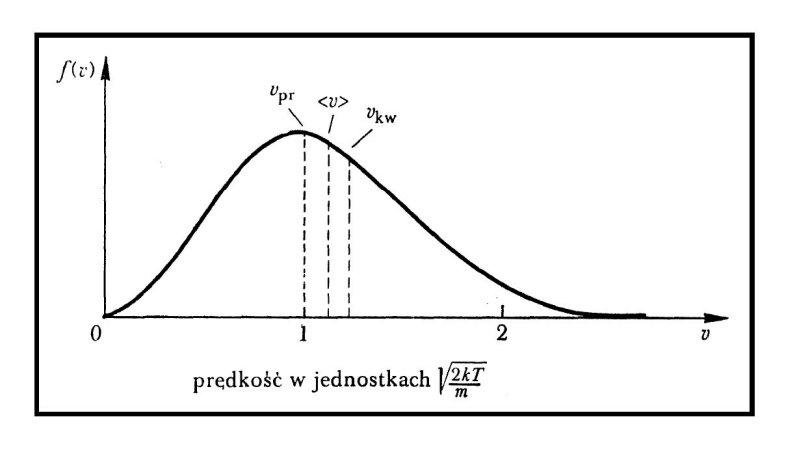
\includegraphics[width=0.6\textwidth]{images/max1.png}
\end{figure}

\begin{figure}[H]
    \centering
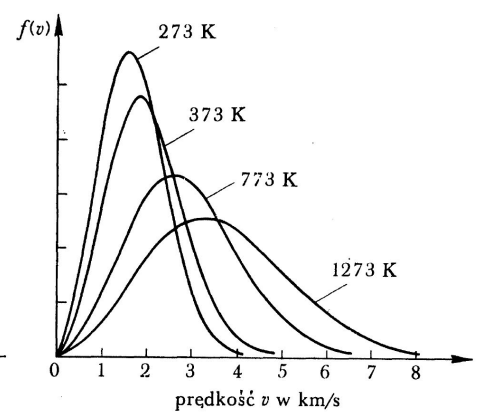
\includegraphics[width=0.4\textwidth]{images/max2.png}
\end{figure}
Związek temperatury z energią kinetyczną cząsteczek gazu.
\begin{equation*}
    \langle E_\mathrm{k} \rangle = \frac{3}{2}k_\mathrm{B}T
\end{equation*}


Prędkość najbardziej prawdopodobna to maksimum rozkładu Maxwella:
\begin{equation*}
    v_\text{pr}=\sqrt{\frac{2kT}{m}}
\end{equation*}
\section{Statystyki kwantowe; bozony i fermiony.}
\url{https://home.agh.edu.pl/~zak/downloads/FCS-8-2016.pdf}

\begin{figure}[H]
    \centering
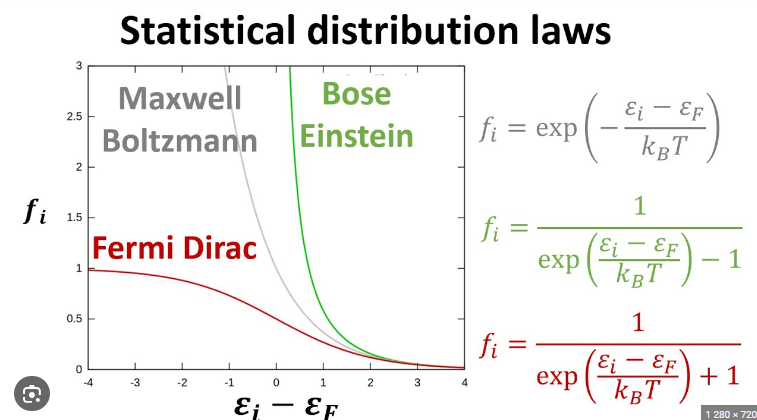
\includegraphics[width=0.8\textwidth]{images/statystyki.png}
\end{figure}

\section{Zjawisko fotoelektryczne i efekt Comptona, energia i pęd fotonu.}

\subsection{Zjawisko fotoelektryczne}

Polega ono na uwalnianiu elektronów z metali pod wpływem światła. Demonstrację zjawiska fotoelektrycznego można wykonać za pomocą układu przedstawionego poniżej. Płytkę cynkową aktywuje się wcierając w jej powierzchnię rtęć, a następnie ustawia się ją w odizolowanym elektrycznie uchwycie. Jeżeli zostanie ona naładowana ładunkiem ujemnym, a następnie oświetlona nadfioletem, to ulega szybkiemu rozładowaniu. Tą samą płytkę, ale naładowanej dodatnio, nie można rozładować przez oświetlanie.  \\
Wynika, że pod wpływem światła elektrony w płytce stają się swobodne. Ujemnie naładowana płytka uwalnia elektrony do otaczającego ją powietrza; dodatnio naładowana płytka utrzymuje je przez przyciągania kulombowskie. \\
Prąd generowany przez elektrony swobodne, jako funkcja częstości światła, zaczyna się przy pewnej częstości granicznej, która jest wielkością charakterystyczną dla materiału elektrody. Kiedy potencjał hamujący osiąga pewną wartość wystarczającą do powstrzymywania elektronów przed opuszczeniem płytki, fotoprąd maleje do zera i tak już pozostaje. \\
Na gruncie fizyki klasycznej można oczekiwać, że pole elektryczne światła, które jest proporcjonalne do pierwiastka kwadratowego z natężenia światła, jest odpowiedzialne za przyspieszanie i uwalnianie elektronów z elektrody. Energia elektronów powinna wzrastać ze wzrostem natężenia światła. Okazuje się jednak, że energia fotoelektronów nie zależy od natężenia światła, lecz jedynie od jego częstości. Z drugiej strony liczba emitowanych elektronów jest proporcjonalna do natężenia światła. \\
Fotoelektrony są emitowane jedynie wtedy gdy częstość światła  jest wyższa niż charakterystyczna wartość graniczna. Musi być zatem spełniona zależność:
\begin{equation*}
    h\nu \geq h\nu_g=eV_A
\end{equation*}

\subsection{Zjawisko Comptona}

\url{https://home.agh.edu.pl/~kakol/efizyka/w32/main32e.html}
Nazwę zjawiska Comptona nadano zjawiskom rozpraszania promieniowania elektromagnetycznego przez słabo związane lub swobodne elektrony. Jest ono charakterystyczne dla obszaru promieniowania rentgenowskiego widma promieniowania elektromagnetycznego. Padająca fala wzbudza elektrony w atomach tarczy, wprawiając je w oscylacje. Oscylujące elektrony w polu dodatnio naładowanego jądra atomowego mogą być traktowane jak oscylatory klasyczne; emitują one promieniowanie o częstości takiej samej, jaka pobudziła je do wykonywania oscylacji. Takie zjawisko nazywa się rozpraszaniem światła Rayleigha. \\
Compton zaobserwował, że w rozproszonym promieniowaniu oprócz promieniowania o nie zmienionej długości fali pojawia się składowa o zmienionej długości fali. Zachodzi przy tym prosta relacja pomiędzy zmianą długości fali w wyniku rozpraszania a kątem rozpraszania, i to niezależnie od materiału tarczy:
\begin{equation*}
    \Delta \lambda = \lambda_C(1-\cos \theta),
\end{equation*}
gdzie $\lambda_C=0,0024$ nm nosi nazwę komptonowskiej długości fali. Zmiana długości $\Delta \lambda$ jest również całkowicie niezależna od pierwotnej długości fali promieniowania. Tylko natężenie promieniowania w zjawisku rozproszenia Comptona zależy od materiału tarczy - jest ono szczególnie duże dla lekkich materiałów (o małym Z) w porównaniu z absorpcją promieniowania rentgenowskiego, która w przybliżeniu rośnie jak $\mathrm{Z^3}$. 

\begin{figure}[H]
    \centering
    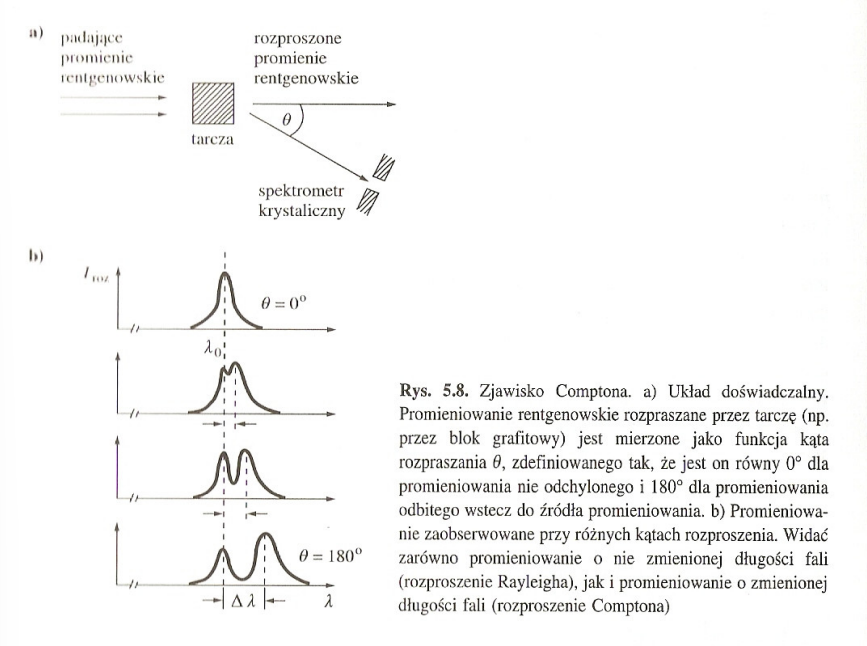
\includegraphics[width=0.8\textwidth]{compton.png}
    \label{fig:compton}
\end{figure}

Zmiana długości fali jest maksymalna dla $\theta=180\degree$. Gdy energia kwantów promieniowania przed rozproszeniem wynosi 1000 eV, energia promieniowania rozproszonego pod kątem 180 \degree jest równa 996 eV, a przy energii pierwotnej 1 MeV energia ta będzie równa 200 keV. W pierwszym wypadku energia została zmniejszona o 4 eV, a w drugim o 800 keV. W obu wypadkach odpowiednia zmiana długości fali jest równa około $\Delta \lambda=0,005$ nm. Wyjaśnienie tych doświadczeń nie było możliwe w ramach falowego obrazu światła. W ramach hipotezy o kwantach promieniowania zjawisko to można opisać jako zderzenie pomiędzy dwoma cząstkami: fotonem i elektronem. Podczas zderzenia przenoszone są pęd i energia. \\

\begin{figure}[H]
    \centering
    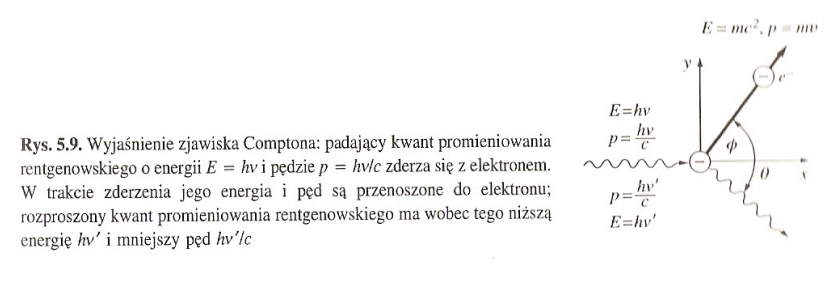
\includegraphics[width=0.8\textwidth]{compton1.png}
    \label{fig:compton1}
\end{figure}
Ściślej mówiąc, mamy do czynienia ze sprężystym zderzeniem pomiędzy fotonami i ze słabo związanymi elektronami na zewnętrznych powłokach elektronowych w atomach; ich prędkość początkowa jest $v_0 \approx 0$. Zakłada się przy tym, że energia wiązania elektronów jest mała i że można ją zaniedbać w porównaniu z energią fotonów.


\section{Hipoteza de Broglie’a, dualizm korpuskularno-falowy.}
Z analizy rozpraszania Comptona i efektu fotoelektrycznego wynika, że fala elektromagnetyczna podczas oddziaływania z materią zachowuje się jak zbiór cząstek, zwanych fotonami. De Broglie zaproponował nową hipotezę, zakładającą, że elektrony i inne cząstki materii mogą zachowywać się jak fale. Ideę tę nazywamy hipotezą de Broglie’a. Zgodnie z hipotezą de Broglie’a wielkości opisujące zarówno bezmasowe fotony, jak i masywne cząstki muszą spełniać taki sam zestaw równań łączących energię $E$ z częstotliwością $\nu$ i pęd $p$ z długością fali $\lambda$. Każdej cząstce o danej energii i pędzie towarzyszy fala de Broglie’a (ang. de Broglie wave) o częstotliwości $\nu$ i długości fali $\lambda$. 

Długość fali de Broglie'a dana jest wzorem:
\begin{equation*}
    \lambda=\frac{h}{mv}.
\end{equation*}

Davisson i Germer. badając odbicie powolnych elektronów od kryształów, zaobserwowali efekty interferencyjne, tzn. maksima i minima natężenia odbitych elektronów, które były w jednoznaczny sposób określone przez prędkości elektronów, orientację kryształu i kąt obserwacji. Maksima interferencji powstają podobnie jak przy dyfrakcji promieni rentgenowskich na płaszczyznach sieciowych. Występowanie interferencji oznacza, że z ruchem elektronów muszą się łączyć zjawiska falowe. Istotnie, de Broglie wysunął sugestie, że tak jak światło może mieć korpuskularną naturę, również elektrony muszą mieć charakter falowy; założył słuszność podstawowej relacji $p=h/\lambda$ pomiędzy pędem a długością fali. \\
Hipoteza de Broglie'a stosuje się do wszystkich cząstek, a nie tylko do elektronów. 


\section{Grupy punktowe symetrii, grupy Lauego, grupy dyfrakcyjne i grupy przestrzenne. Typy komórek Bravais. Notacje stosowane do opisu grupy symetrii punktowej.}

\subsection{Grupy punktowe symetrii}

Ze względu na parametry komórki elementarnej (a, b, c, $\alpha,\; \beta, \; \gamma$) wszystkie kryształy możemy zaliczyć do jednego z 7 układów krystalograficznych. Analizując rozkład cząsteczek w komórce elementarnej można zdefiniować 4 typy komórek translacyjnych: P, A(B,C), F oraz I. Jeśli rozważyć komórki translacyjne możliwe w poszczególnych układach krystalograficznych, to mamy 14 sieci translacyjnych Bravais. Analiza rozkładu materii w komórce elementarnej w przestrzeni trójwymiarowej prowadzi do wyróżnienia 32 grup punktowych symetrii. \\

W kryształach występują kombinacje: osi symetrii, osi symetrii i osi symetrii inwersyjnych, osi symetrii i środka symetrii. Klasy symetrii są to różne, możliwe w kryształach kombinacje makroskopowych elementów symetrii przecinających się w jednym punkcie. Klasy symetrii nazywa się grupami punktowymi lub klasami krystalograficznymi. Sieciowa budowa kryształów powoduje, że liczba klas symetrii jest ograniczona, możliwe są jedynie 32 grupy punktowe w ich skład wchodzą
elementy symetrii makroskopowej: pięć osi symetrii (1, 2, 3, 4, 6) i pięć osi inwersyjnych $\mathrm{(\Bar{1}, \Bar{2}, \Bar{3}, \Bar{4}, \Bar{5}, \Bar{6})}$ oraz 22 dozwolone oryginalne kombinacje elementów symetrii makroskopowej. 

\subsection{Grupy Lauego}
W metodzie Lauego na nieruchomy kryształ pada polichromatyczna wiązka promieniowanie rentgenowskiego. Obraz dyfrakcyjny rejestruje się na płaskiej błonie fotograficznej ustawionej prostopadle do kierunku promieni pierwotnych. \\

Istnieje tylko 10 różnych typów symetrii laugramów (otrzymane rentgenogramy), które nazywają się obrazami Lauego. Obrazy Lauego oznacza się symbolami międzynarodowymi: 1, 2, 3, 4, 6, m, 2mm, 3m, 4mm, 6mm. Obraz 1 jest obrazem asymetrycznym i powstaje, gdy w krysztale nie występuje żaden element symetrii równoległy do wiązki padającej. Gdy promienie rentgenowskie biegną w krysztale równolegle do osi 2, 3, 4 i 6-krotnej, wówczas otrzymuje się obrazy typu 2, 3, 4 i 6. Gdy promienie rentgenowskie biegną równolegle do płaszczyzny symetrii, wówczas otrzymuje się obraz typu m. Gdy padające promienie rentgenowskie są równoległe do osi n–krotnej, wzdłuż której przecina się n płaszczyzn symetrii, wówczas otrzymuje się obrazy typu 2mm, 3m, 4mm i 6mm.

\begin{figure}[H]
    \centering
    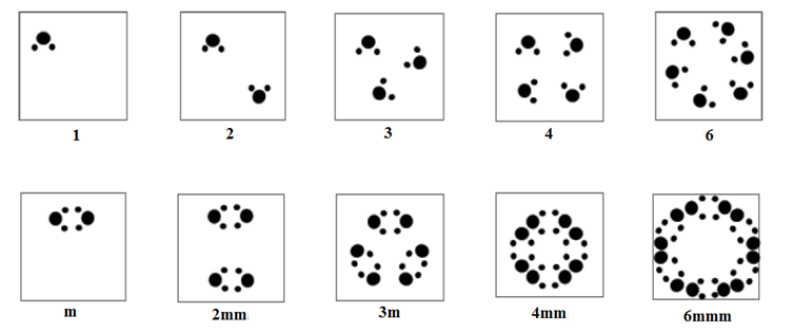
\includegraphics[width=\textwidth]{obrazy_lauego.png}
    \caption{Typy obrazów Lauego}
    \label{fig:laue}
\end{figure}
W oparciu o symetrię obrazów Lauego przyporządkowuje się badany kryształ do jednej z 11 klas dyfrakcyjnych, zwanych klasami Lauego: $\mathrm{\Bar{1}}$, 2/m, mmm, 4/m, 4/mmm, $\mathrm{\Bar{3}}$, $\mathrm{\Bar{3}m}$, 6/m, 6/mmm, m3, m3m. \\

\url{https://www.krystalografia.us.edu.pl/mag/mag9.pdf}


\subsection{Typy komórek Bravais}

Sieć translacyjna Bravais'go określa charakter okresowego uporządkowania w przestrzeni powtarzających się elementów strukturalnych kryształu. Stanowi nieskończony zbiór punktów przestrzeni uporządkowanych w ten sposób, że przy obserwacji układu z dowolnego należącego doń punktu wzajemne rozmieszczenie punktów układu i jego orientacja są zawsze takie same. \\
Biorąc pod uwagę możliwe centrowanie komórki elementarnej, w przestrzeni trójwymiarowej jest możliwych tylko 14 typów translacyjnych sieci przestrzennych zwanych sieciami Bravais'go. Każdy z 14 typów sieci przestrzennych Bravais'go ma swoją charakterystyczną komórkę elementarną, która ze względu na parametry sieci przestrzennej jest podporządkowana jednemu z 7 układów krystalograficznych (Tablica 1). \\
Komórki elementarne mogą zawierać węzły tylko w narożach, zawierać dodatkowe węzły w środku geometrycznym, na środkach dwóch przeciwległych ścian lub na środkach wszystkich ścian. Komórki zawierające węzły tylko w narożach nazywamy prymitywnymi, natomiast komórki z dodatkowymi węzłami komórkami złożonymi. \\
Jeżeli węzeł występuje w środku geometrycznym komórki wówczas komórkę tą nazywamy wewnętrznie (przestrzennie) centrowaną i oznaczamy symbolem I. Jeżeli dodatkowe węzły występują na środkach wszystkich ścian komórki nazywamy ją przestrzennie centrowaną i oznaczamy literą F. Komórki o centrowanych dwóch przeciwległych ścianach (001) oznaczamy literą C, natomiast komórki o centrowanych dwóch przeciwległych ścianach (100) i (010) oznaczamy odpowiednio literami A i B. 

\begin{figure}[H]
    \centering
    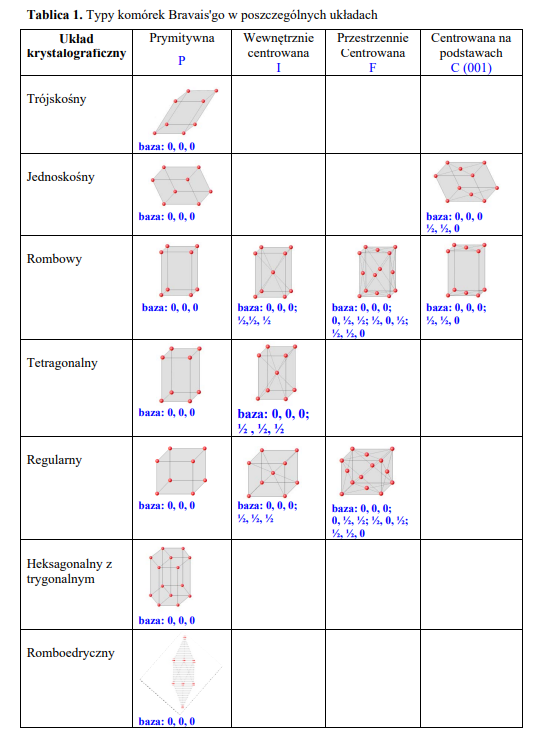
\includegraphics[width=\textwidth]{bravais.png}
    \label{fig:kryst}
\end{figure}


\section{Pomiar w mechanice kwantowej (obserwable); zasada nieoznaczoności.}
\textbf{Obserwabla} to operator hermitowski, czyli operator, który jest równy swojemu sprzężeniu ($\hat{C}^\dagger=\hat{C}$). Obserwabla jest operatorem hermitowskim, który wyznacza bazę w przestrzeni Hilberta, czyli przestrzeni wektorowej z iloczynem skalarnym, która opisuje fizyczny stan układu w chwili czasu. Bazę tę wyznaczają wektory własne tej obserwabli. 

Każdej mierzonej wielkości fizycznej $\mathcal{A}$ odpowiada operator hermitowski, będący obserwablą: $\mathcal{A} \longleftrightarrow \hat{A}$. 

Przykład:
\begin{equation*}
    E_\text{kin}=\frac{p^2}{2m}\quad\leftrightarrow\quad\hat{H}_\text{kin}=\frac{\hat{p}^2}{2m}
\end{equation*}

Możliwymi wynikami pomiaru $\mathcal{A}$ są tylko wartości własne $\hat{A}$.

\begin{figure}[H]
    \centering
    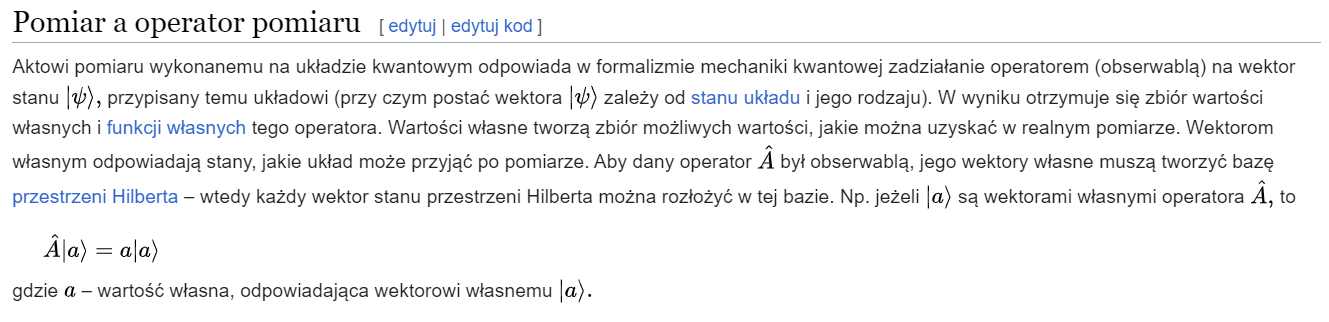
\includegraphics[width=\textwidth]{images/obserwabla.png}
\end{figure}

$|a\rangle $ -- wektor, który opisuje stan układu.


\textbf{Zasada nieoznaczoności} głosi, że niemożliwy jest absolutnie ścisły jednoczesny pomiar położenia i pędu elektronu. Dolne ograniczenie jednoczesnej mierzalności tych dwóch wielkości jest dane wzorem: $\Delta x \Delta p \geq \hbar/2$ ($\Delta x$ -- dyspersja położenia, $\Delta p $  -- dyspersja pędu). Gdybyśmy chcieli, aby $\Delta x$ osiągnęło 0 (ścisłe wyznaczenie położenia), musielibyśmy pozwolić, aby $\Delta p$ osiągnęło nieskończoność i vice versa.

Kryszewski 49

\section{Równanie Schrödingera, funkcja falowa i jej interpretacja.}

\subsection{Funkcja falowa}

Przypomnijmy w tym miejscu, że w mechanice klasycznej układ fizyczny jest opisany zbiorem współrzędnych i pędów uogólnionych. Np. cząstka klasyczna jest opisana przez trzy składowe położenia $\overrightarrow{x}(t)$ i trzy składowe pędu $\overrightarrow{p}(t)$, a więc łącznie przez 6 funkcji czasu. Zależność od czasu współrzędnych i pędów uogólnionych wynika np. z hamiltonowskich równań ruchu. Są to równania różniczkowe, które pozwalają jednoznacznie i ściśle przewidzieć późniejszy stan układu, pod warunkiem, że znany jest stan w pewnej chwili wcześniejszej (początkowej). Współrzędne uogólnione są sparametryzowane czasem, więc wyznaczają trajektorię układu w funkcji czasu. Przechodząc do zjawisk mikroświata radykalnie zmieniamy sposób jego opisu.
Postulujemy, że układ fizyczny (na razie skupimy uwagę na pojedynczej cząstce) jest w pełni opisany za pomocą tzw. funkcji falowej, którą zwykle oznaczamy jako $\psi(\overrightarrow{r},t)$. Mówimy też czasem, że stan układu jest dany funkcją falową $\psi(\overrightarrow{r},t)$. \\

Wektor $\overrightarrow{r}$ występujący jako argument funkcji falowej nie wiąże się w żaden prosty sposób z położeniem cząstki. Funkcja falowa może także zależeć od innych wielkości (parametrów), ale od ilu i jakich, zależy od tego jaki układ fizyczny chcemy opisywać. Stan kwantowo-mechaniczny układu (a więc funkcja falowa) to nieskończenie wiele liczb – wartości funkcji falowej we wszystkich dopuszczalnych punktach ~r dla kolejnych chwil czasu t. Należy tutaj podkreślić, że kwantowo-mechaniczna funkcja falowa może w ogólności być funkcją zespoloną.

\begin{figure}[H]
    \centering
    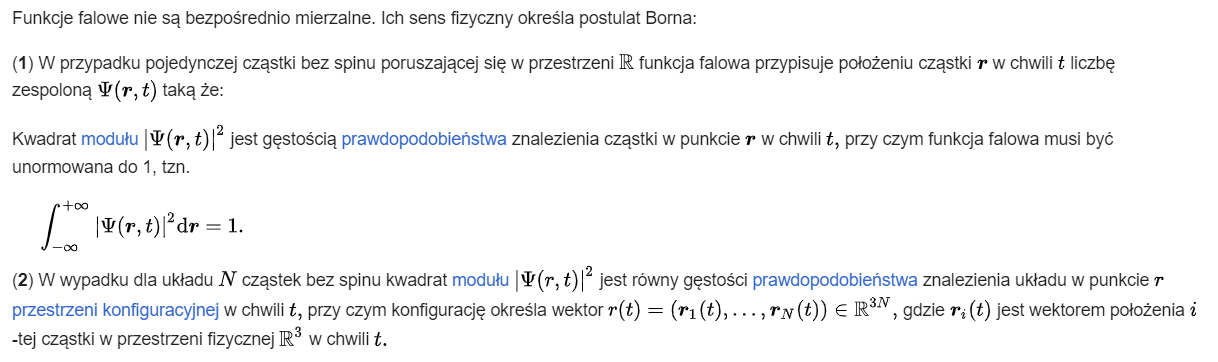
\includegraphics[width=\textwidth]{images/funk_fal.png}
\end{figure}

\subsection{Równanie Schrödingera}

W jaki sposób wyznaczać funkcje falowe? Musimy dysponować odpowiednim równaniem, które będzie spełnione przez funkcje falowe. Innymi słowami, potrzebujemy równania, którego rozwiązaniami będą funkcje falowe. Skupmy na razie uwagę na pojedynczej, bezspinowej cząstce o masie m poruszającej się w pewnym polu tak, że jej energia potencjalna opisywana jest funkcją $V=V(\overrightarrow{r},t)$ - funkcją argumentu $\overrightarrow{r}$ i czasu. \\
Postulujemy, że funkcja falowa $\psi(\overrightarrow{r},t)$ odpowiadająca rozważanej cząstce spełnia równanie Schrödingera:
\begin{equation*}
    i\hbar \frac{\partial}{\partial t}\psi(\overrightarrow{r},t) = -\frac{\hbar^2}{2m}\nabla^2\psi(\overrightarrow{r},t)+V(\overrightarrow{r},t)\psi(\overrightarrow{r},t).
\end{equation*}
Można go też zapisać za pomocą operatora Hamiltona (hamiltonian) dla cząstki o masie m poruszającej się w polu, w którym ma ona energię potencjalną $V(\overrightarrow{r},t)$:
\begin{equation*}
    i\hbar \frac{\partial}{\partial t}\psi(\overrightarrow{r},t) = \hat{H}\psi(\overrightarrow{r},t).
\end{equation*}

\textbf{Równanie Schrödingera} - pozwala nam na opis ewolucji stanu układu kwantowego w czasie.

Równanie Schrödingera zależne od czasu:
\begin{figure}[H]
    \centering
    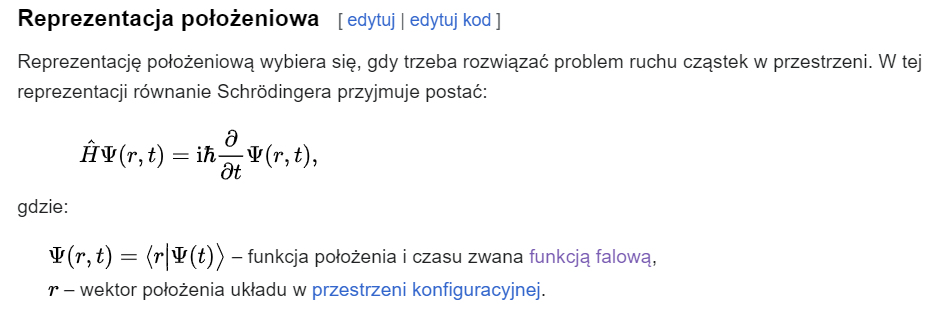
\includegraphics[width=\textwidth]{images/schr1.png}
\end{figure}

Równanie Schrödingera niezależne od czasu:
\begin{figure}[H]
    \centering
    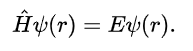
\includegraphics[width=0.2\textwidth]{images/schr2.png}
\end{figure}

\begin{figure}[H]
    \centering
    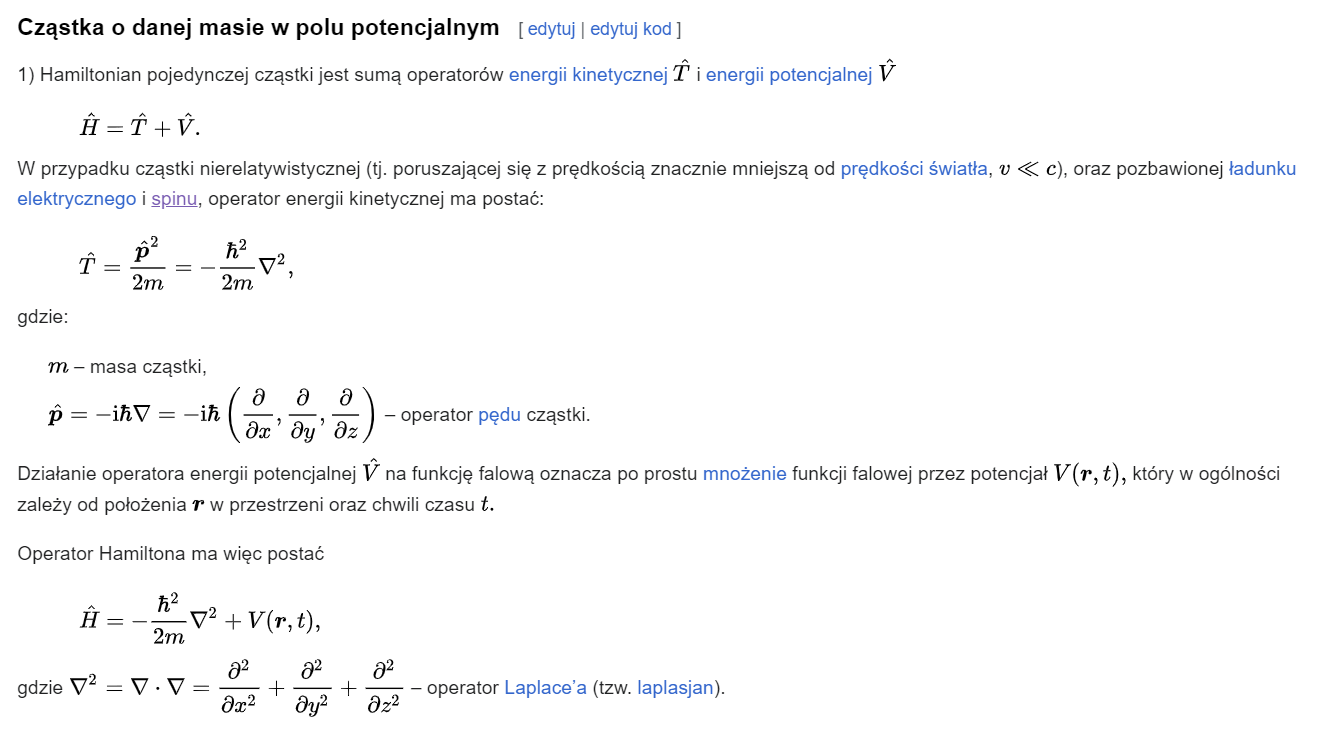
\includegraphics[width=\textwidth]{images/schr3.png}
\end{figure}


\section{Kwantowy oscylator harmoniczny - funkcje falowe, energia oscylatora.}
\url{https://www.youtube.com/watch?v=l29vbExLSak&t=258s}
\section{Atom wodoru w mechanice kwantowej.}
\begin{figure}[H]
    \centering
    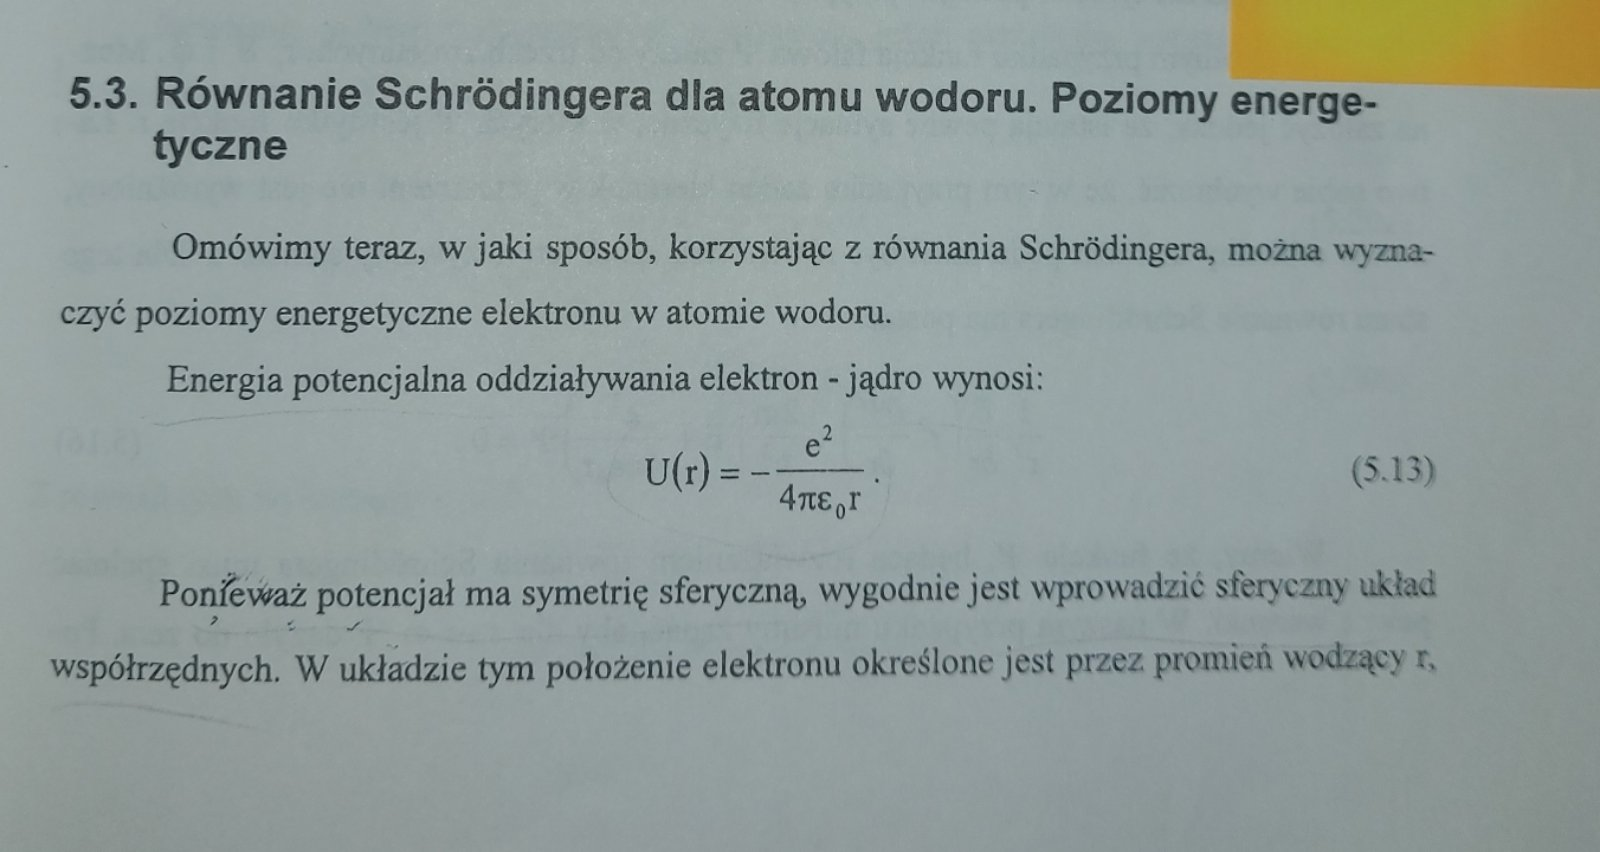
\includegraphics[width=\textwidth]{images/wodor1.jpg}
\end{figure}
\begin{figure}[H]
    \centering
    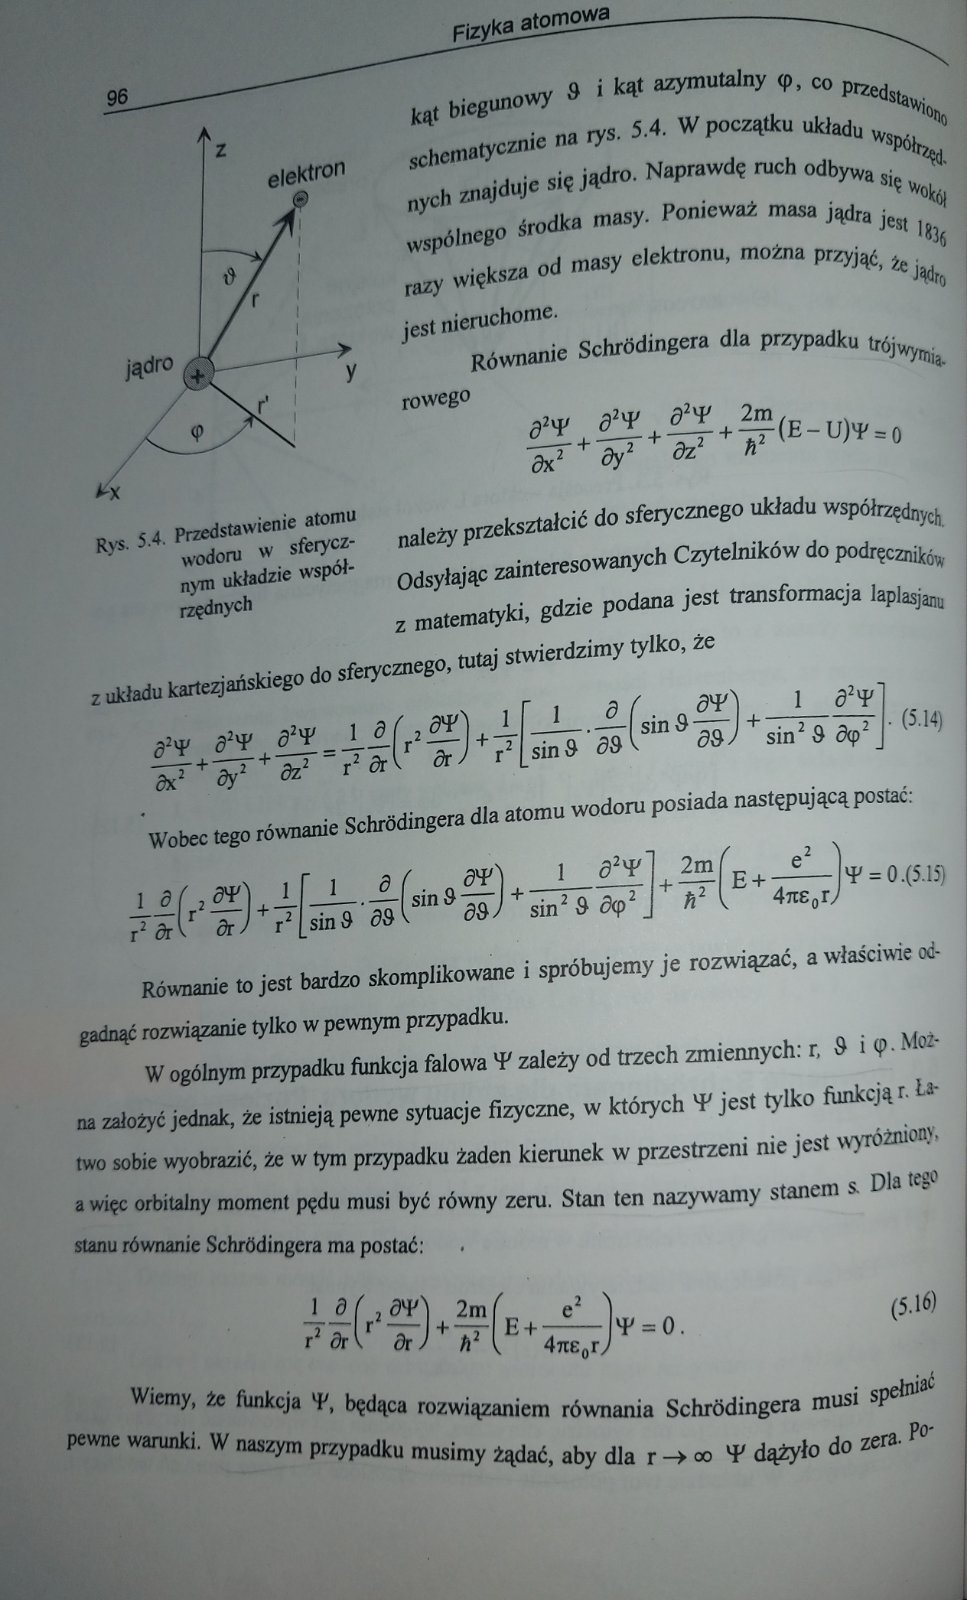
\includegraphics[width=\textwidth]{images/wodor2.jpg}
\end{figure}
\begin{figure}[H]
    \centering
    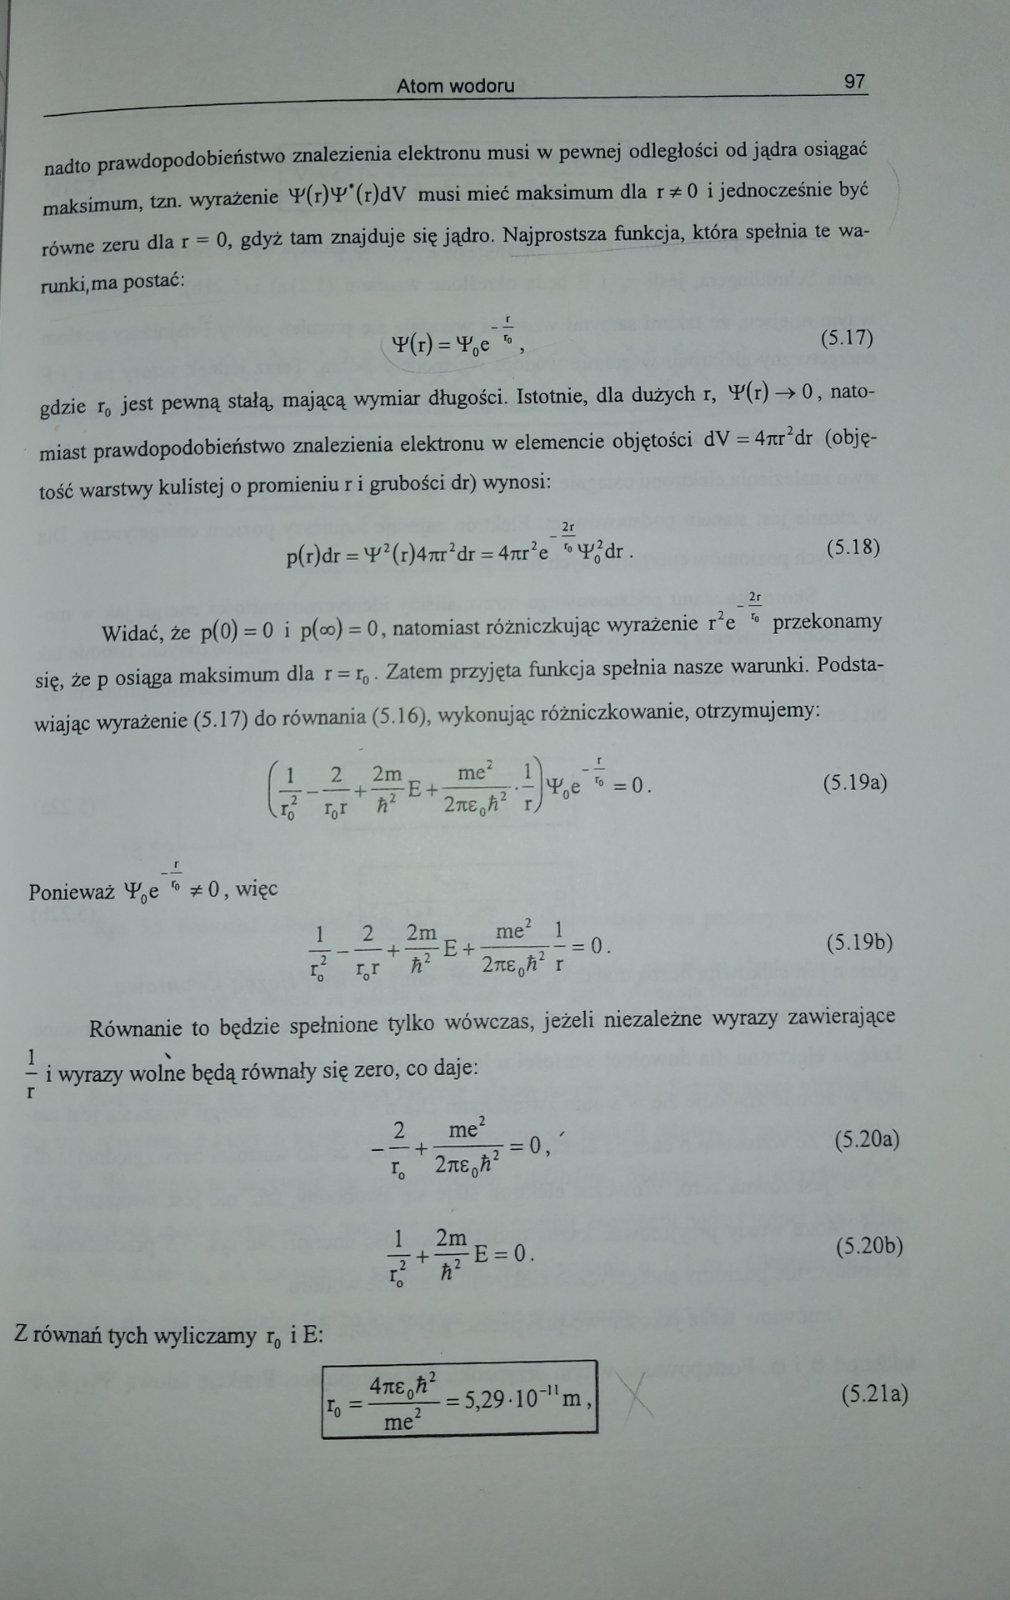
\includegraphics[width=\textwidth]{images/wodor3.jpg}
\end{figure}
\begin{figure}[H]
    \centering
    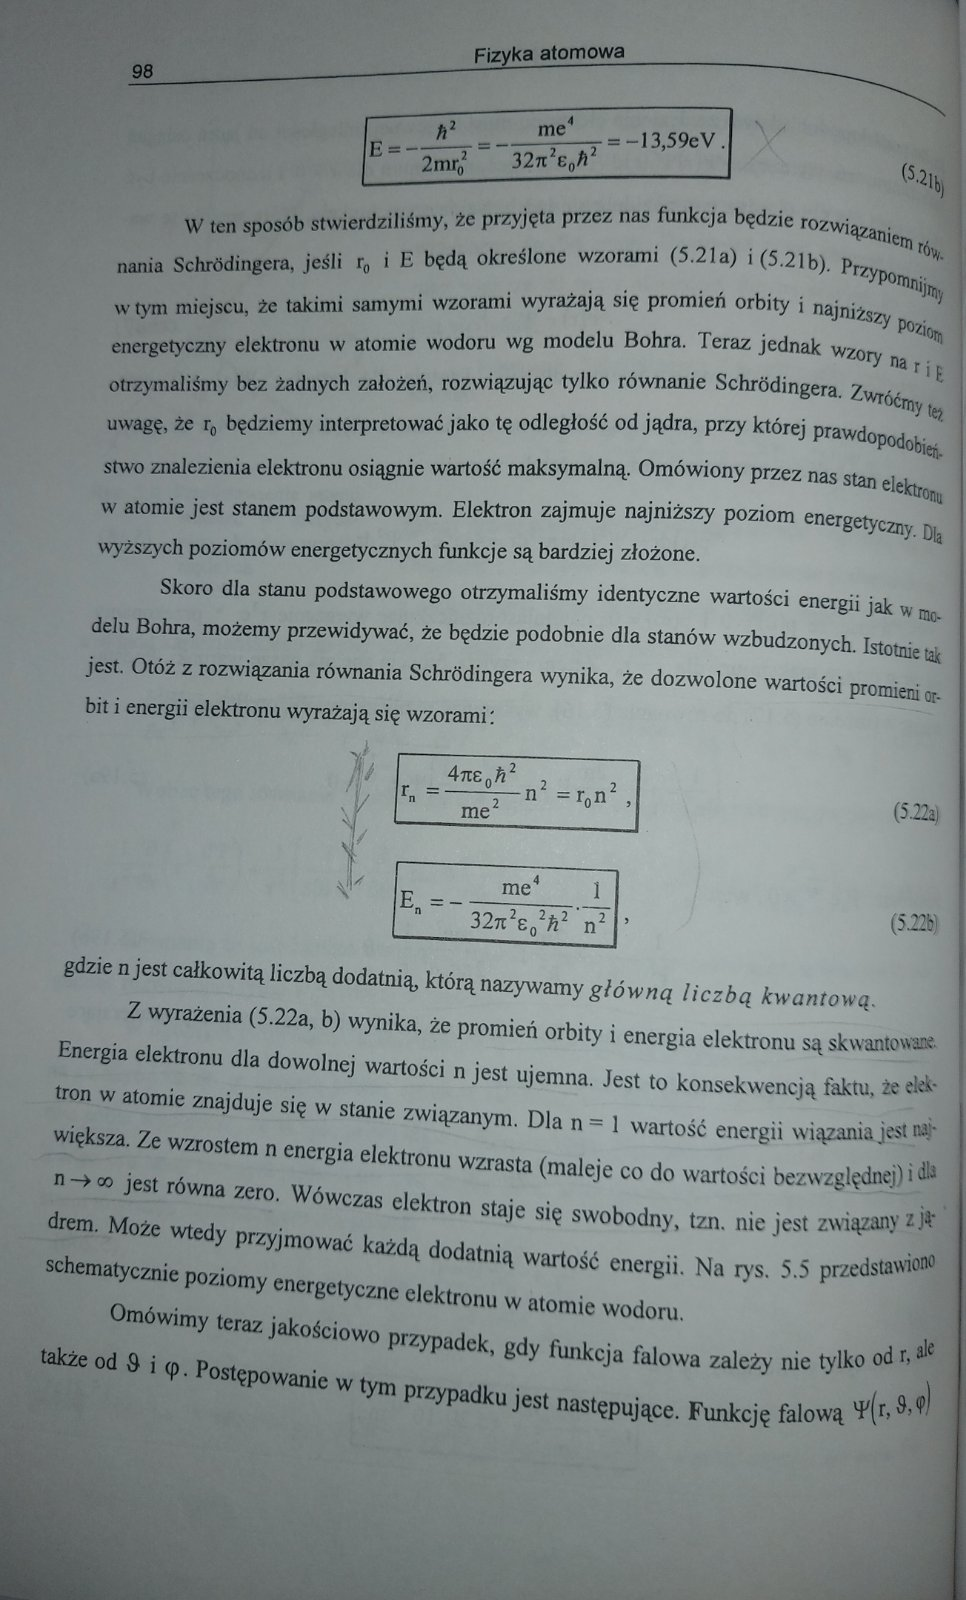
\includegraphics[width=\textwidth]{images/wodor4.jpg}
\end{figure}
\begin{figure}[H]
    \centering
    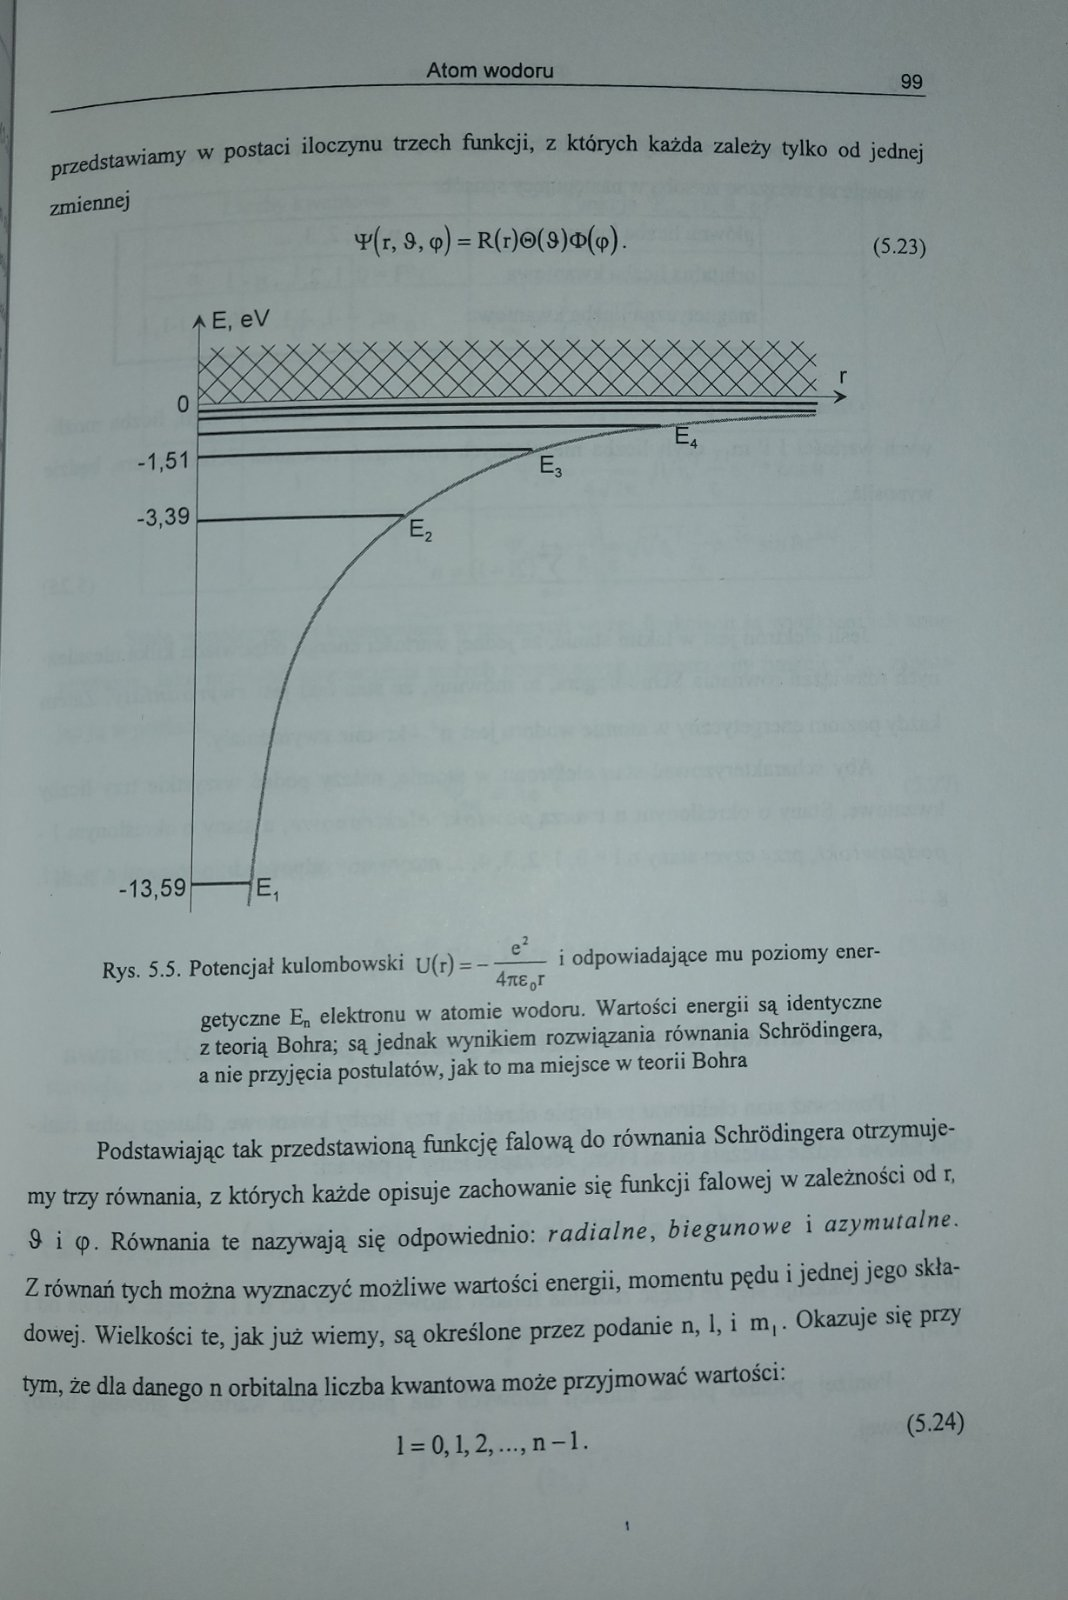
\includegraphics[width=\textwidth]{images/wodor5.jpg}
\end{figure}
\begin{figure}[H]
    \centering
    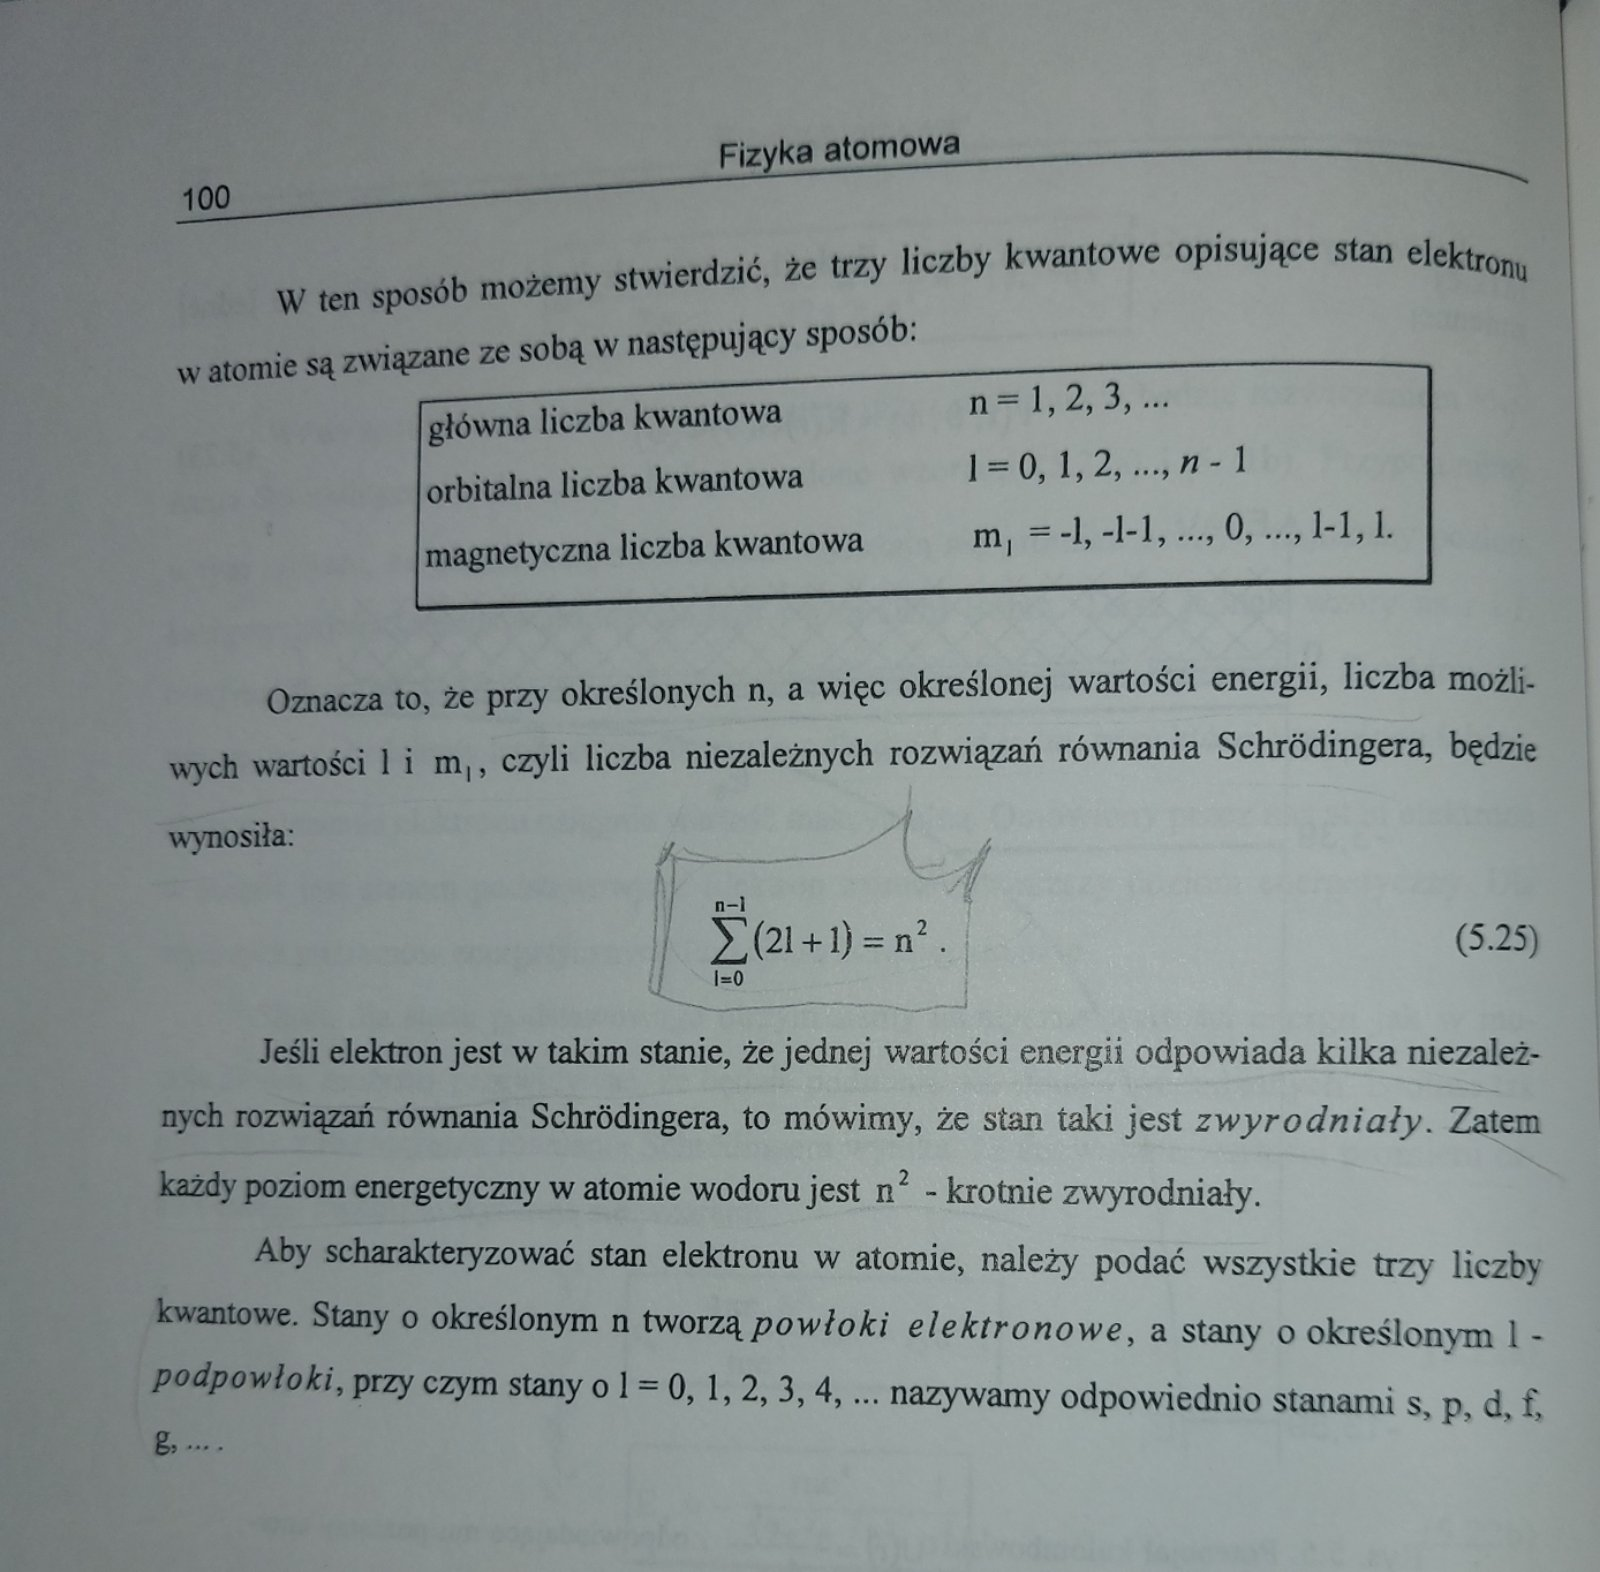
\includegraphics[width=\textwidth]{images/wodor6.jpg}
\end{figure}

\section{Atom w zewnętrznym polu elektrycznym i magnetycznym – zjawisko Starka, zjawisko Zeemana.}

\url{http://www.ftj.agh.edu.pl/~wolny/Wc71691e281a7b.htm}

\section{Stany energetyczne atomów; absorpcja i emisja promieniowania elektromagnetycznego; emisja spontaniczna i wymuszona.}



W przybliżeniu nierelatywistycznym stany stacjonarne atomu wyznaczone są przez równanie Schrödingera dla układu elektronów poruszających się w kulombowskim polu jądra i oddziałujących ze sobą siłami elektrostatycznymi. Każdy stan stacjonarny atomu będzie charakteryzowany określoną wartością całkowitego momentu pędu oraz całkowitą wartością spinu elektronów (S). Same wartości całkowitego momentu pędu i spinu nie determinują jednoznacznie energii stanu. Każdy poziom energetyczny może być zdegenerowany odpowiednio do różnych możliwych kierunków w przestrzeni wektorów L i S. Krotności degeneracji ze względu na te kierunki wynoszą odpowiednio 2L + 1 i 2S + 1, a całkowita krotność zwyrodnienia jest równa iloczynowi (2L + 1)(2S + 1) dla stanu o danych L i S. Ponieważ elektromagnetyczne oddziaływanie elektronów charakteryzują efekty relatywistyczne to energia atomu zależy nie tylko od wielkości wektorów L i S lecz także od ich wzajemnego położenia. W takim razie orbitalny moment pędu i spin atomu, każdy z osobna nie jest zachowany, a zachowanie dotyczy całkowitego momentu pędu J = L + S. W związku z tym poziomy energetyczne atomu charakteryzują się wartościami J całkowitego momentu pędu. Jednak efekty relatywistyczne są względnie małe, i można je traktować jako zaburzenia. Pod wpływem takiego zaburzenia zdegenerowany poziom o danych L i S rozszczepia się na szereg bliskich sobie poziomów, różniących się wartościami całkowitego momentu pędu J. \\

W pierwszym przybliżeniu bezwzględne wartości orbitalnego momentu pędu i spinu, ale nie ich kierunki, są zachowane co pozwala na charakteryzowanie poziomów energetycznych atomu wartościami L i S. Wynikiem efektów relatywistycznych jest rozszczepienie się poziomu o danych wartościach L i S na szereg poziomów o różnych wartościach J, czyli pojawienie się struktury subtelnej poziomów. J przyjmuje wartości od L + S do |L – S|, zatem poziom o danych L i S rozszczepia się na 2S + 1, jeżeli L > S lub 2L + 1, gdy L < S, różnych poziomów. Każdy z tych poziomów jest zwyrodniały 2J + 1 razy ze względu na kierunek wektora J.
Atomowe poziomy energetyczne, czyli termy atomowe, oznacza się symbolami analogicznymi do tych stosowanych do oznaczania pojedynczych stanów cząstek o określony wartościach momentu pędu. Mamy więc stany o różnych wartościach całkowitego momentu pędu:

L	=	0	1	2	3	4	5	...
 	 	S	P	D	F	G	H	...

\section{Elektryczne i magnetyczne właściwości substancji: Trwałe i indukowane momenty dipolowe cząsteczki. Względna przenikalność elektryczna. Paramagnetyzm, diamagnetyzm, ferromagnetyzm. Podatność magnetyczna. Prawo Curie.}
\url{https://home.agh.edu.pl/~nmos1/FUK/fizykochemia_powierzchni_skany/03/t_dutkiewicz_fizykochemia_powierzchni_rozdzial3.pdf}\\
\url{https://openstax.org/books/fizyka-dla-szk%C3%B3%C5%82-wy%C5%BCszych-tom-2/pages/8-5-mikroskopowy-model-dielektryka}

\section{Budowa jądra atomowego. Rozpady jąder atomowych (promieniowanie alfa, beta i gamma). Rozszczepienie jąder ciężkich: reakcje łańcuchowe, reaktor jądrowy, masa krytyczna.}

\section{Rodzaje cząstek elementarnych: leptony i hadrony i kwarkowa teoria budowy hadronów.}
\textbf{Leptony} - grupa 12 cząstek elementarnych (6 cząstek i 6 antycząstek), należących do grupy fermionów fundamentalnych, razem z kwarkami. Do leptonów zaliczają się:
\begin{itemize}
\item elektron ($e^-$), mion ($\mu^-$), taon ($\tau^-$);
\item trzy neutrina odpowiadające każdej z nich: neutrino elektronowe ($\nu_e$), mionowe ($\nu_{\mu}$) oraz taonowe ($\nu_{\tau}$);
\item odpowiadające im antycząstki: pozyton (antyelektron), antymion, antytaon i trzy antyneutrina.
\end{itemize}
\begin{figure}[H]
    \centering
    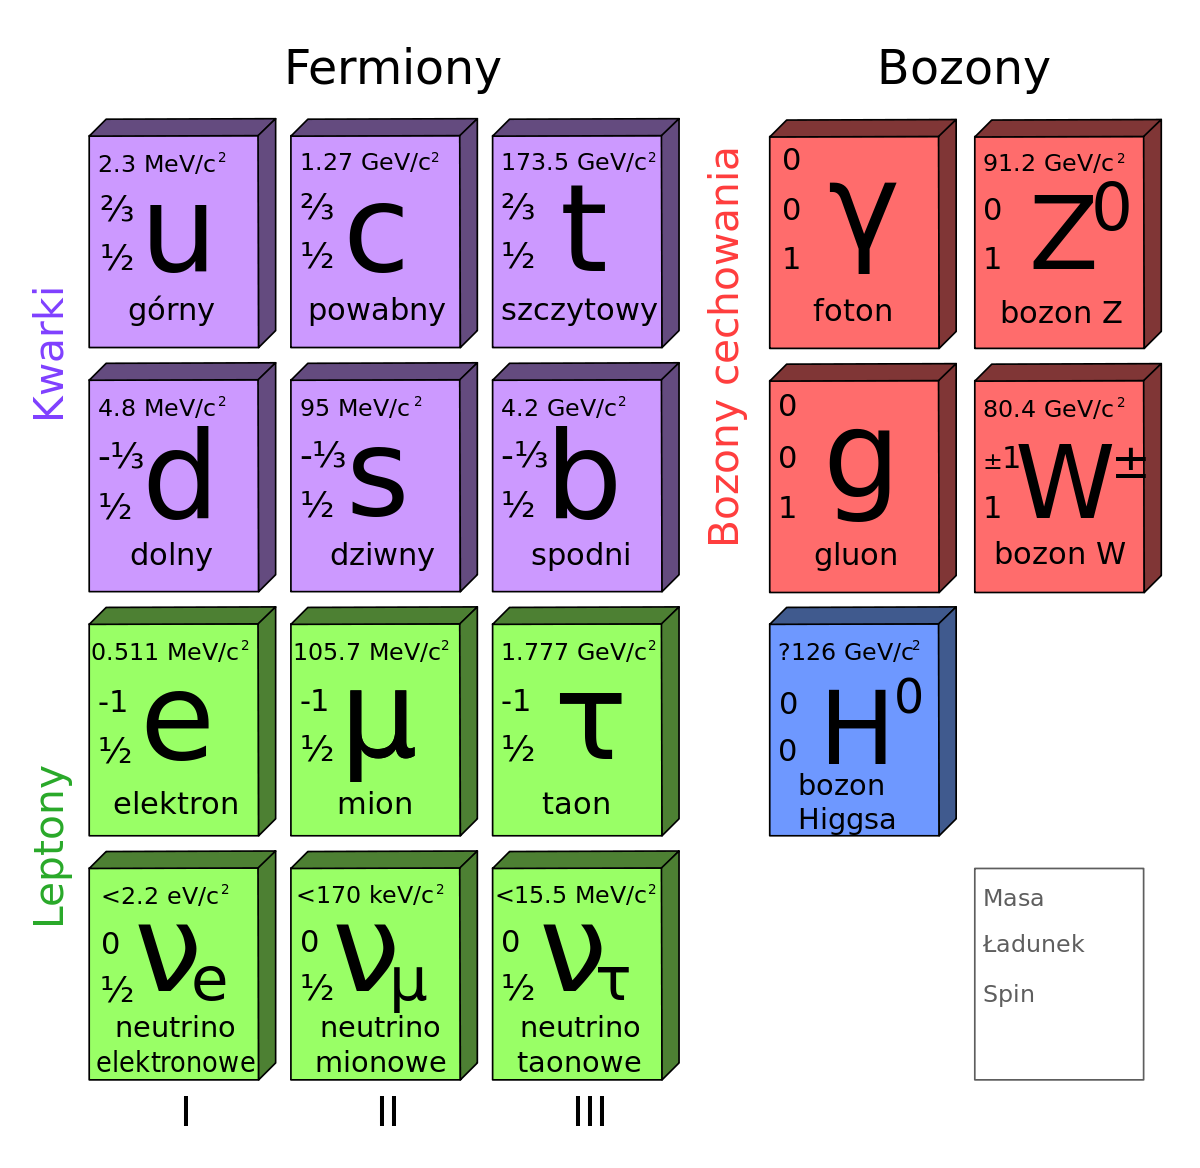
\includegraphics[width=0.8\textwidth]{ModelStd.png}
\end{figure}

\url{http://hep.fuw.edu.pl/II_Pracownia/P3/HTML/index/22%20czastki.htm}

\textbf{Hadrony} - grupa cząstek subatomowych złożonych z dwóch lub więcej kwarków związanych ze sobą za pomocą oddziaływania silnego. Dzielą się na bariony (złożone z nieparzystej liczby kwarków) oraz mezony (złożone z parzystej liczby kwarków). Kwarki charakteryzują się zapachem (górny, dolny, powabny, dziwny, szczytowy (wysoki), spodni (niski)) oraz kolorem (zielony, niebieski, czerwony i 3 antykolory).

Zgodnie z kwarkową teorią budowy hadronów właściwości hadronów są głównie zdeterminowane przez kwarki z jakich są zbudowane. Na przykład proton, będący barionem, zbudowany jest z dwóch kwarków górnych i jednego dolnego (ładunek elektryczny wynosi wtedy 1). Hadrony muszą być "białe" (lub "bezkolorowe") - jest to efekt "uwięzienia koloru". Najprostszym sposobem na zbudowanie białego hadronu jest połączenie 3 kwarków o różnych kolorach (bariony) albo 2 kwarków o danym kolorze/antykolorze (mezony). Wszysktie bariony są fermionami, wszystkie mezony są bozonami.

\section{Układ okresowy pierwiastków. Podział na bloki s, p, d i f. Konfiguracje elektronowe pierwiastków z uwzględnieniem wyjątków: Cr, Cu, Mo, Pd, Ag, Pt, Au}
Nazwy bloków układu kresowego pochodzą od ostatniej podpowłoki obsadzonej w atomie pierwiastka zgodnie z zasadą rozbudowy powłok. 

Atomy należące do tej samej grupy głównej ($s$ i $p$) mają analogiczne konfiguracje powłok walencyjnych, które różnią się tylko wartością $n$. Każdy nowy okres odpowiada obsadzaniu powłoki o nowej głównej liczbie kwantowej. 

\begin{figure}[H]
    \centering
    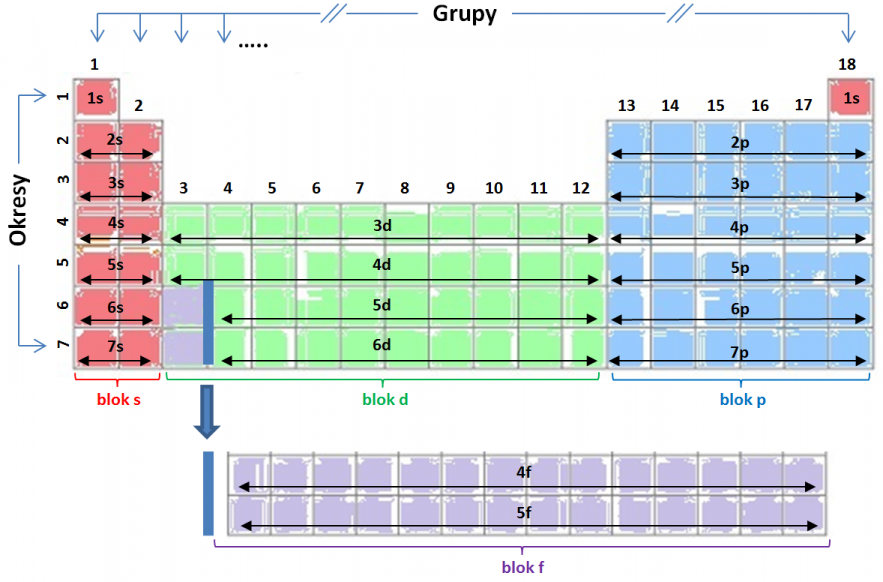
\includegraphics[width=0.8\textwidth]{uklad_okresowy.png}
\end{figure}

\begin{figure}[H]
    \centering
    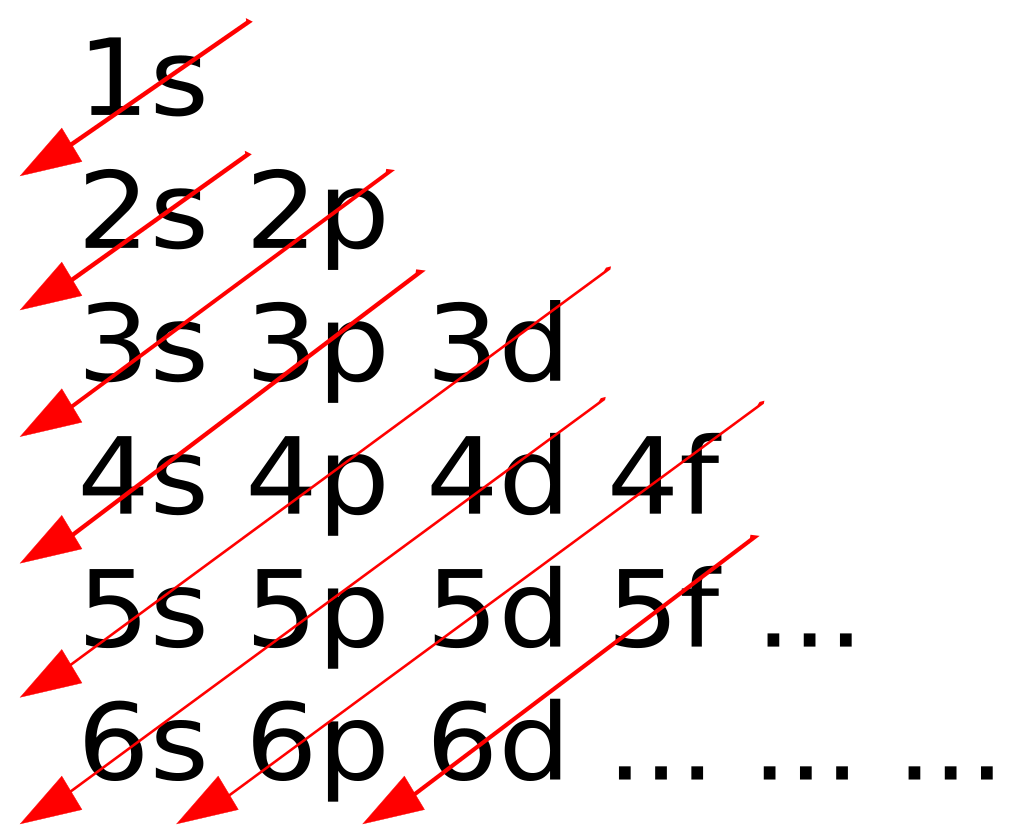
\includegraphics[width=0.4\textwidth]{images/powloki.png}
\end{figure}
Elektron $4s$ przenika przez powłoki wewnętrzne tak skutecznie, że jego energia może być znacznie mniejsza od energii elektronu $4p$ lub $4d$, a nawet od energii elektronu $3d$ tego samego atomu. Dlatego wapń ma np. konfigurację [Ar]$4s^2$. Natomiast skand ma konfigurację [Ar]$3d^14s^2$. Zaczynając od skandu, zapisujemy elektrony $3d$ przed elektronami $4s$: orbitale $3d$ mają tu mniejszą energię niż orbital $4s$ (po $Z=20$), czyli po zapełnieniu orbitalu $4s$ przez dwa elektrony jego energia staje się większa niż orbitalu $3d$.

Stwierdzono doświadczalnie, że zapełniona w połowie powłoka (konfiguracja $d^5$) i całkowicie zapełniona powłoka  d (konfiguracja $d^10$) mają niższą energię, niż wynika to z prostej teorii. W niektórych przypadkach atom ma niższą energię całkowitą, jeżeli podpowłoka $3d$ jest zapełniona w połowie ($d^5$) lub całkowicie ($d^{10}$) w wyniku przeniesienia się do niej elektronu $4s$. Na przykład chrom ma ustaloną doświadczalnie konfigurację [Ar]$3d^54s^1$, a miedź -- konfigurację [Ar]$3d^{10}4s^1$.
Inne wyjątki:
\begin{itemize}
    \item Mo: [Kr]$4d^55s^1$
    \item Pd: [Kr]$4d^{10}$
    \item Ag: [Kr]$4d^{10}5s^1$
    \item Pt: [Xe]$4d^{14}5d^96s^1$
    \item Au: [Xe]$4d^{14}5d^{10}6s^1$
\end{itemize}

\section{Atomy, jony i cząsteczki izoelektronowe. Promienie kowalencyjne i jonowe – definicje, wyznaczanie i zmienność w układzie okresowym. Wpływ rozmiaru i ładunku jonów na właściwości kwasowo-zasadowe ich połączeń.}

Materia nie jest ciągła, lecz składa się z niewyobrażalnie małych cząstek. Najmniejsza cząstka pierwiastka, która może istnieć, nosi nazwę atomu. Pierwiastek jest substancją złożoną z atomów jednego rodzaju. \\
\textbf{Atom} – podstawowy składnik materii. Składa się z małego dodatnio naładowanego jądra o dużej gęstości i otaczającej go chmury elektronowej o ujemnym ładunku elektrycznym.
\textbf{Cząsteczka} to określona, odrębna, obojętna elektrycznie grupa powiązanych ze sobą atomów. \\
\textbf{Jon} to dodatnio lub ujemnie naładowany atom albo grupa powiązanych ze sobą atomów. To atom lub grupa atomów połączonych wiązaniami chemicznymi, która ma niedomiar lub nadmiar elektronów w stosunku do protonów. \\
Cząsteczki/jony, które posiadają taką samą liczbę elektronów walencyjnych i analogiczną
budowę (np. podobny charakter wiązań), określa się jako \textbf{izoelektronowe}, np. CO i CN$^-$. Również atomy mogą być izoelektronowe, przykład: Cl$^-$ i Ar; konfiguracja elektronowa: [Ne]3$s^2$3$p^6$. \\
Mówimy o promieniach atomowych, dogodnych do oceny długości pojedynczego wiązania kowalencyjnego oraz o promieniach jonowych, dogodnych do oceny długości wiązania jonowego. W granicach tego samego okresu, idąc od lewej do prawej, promienie atomów i ich jonów maleją, natomiast przechodząc od okresu do okresu, z uwagi na wzrost liczby kwantowej n, promienie rosną. \\ 

Promienie kowalencyjne odznaczają się większą stałością i zmieniają się tylko nieznacznie przy przejściu od sieci przestrzennej pierwiastka do sieci jego związku. Dzięki temu w bardzo wielu przypadkach promienie atomowe można obliczyć z danych dotyczących budowy cząsteczek związków gazowych lub stałych. \\

\textbf{Promień jonowy} to odległość najbardziej oddalonych elektronów od jądra atomu, w przypadku jonów utworzonych z jednego atomu, lub też od geometrycznego centrum jonów, złożonych z większej liczby atomów.

Promienie jonowe kationów są mniejsze od promienia atomu, od którego pochodzą te jony. Im większy ładunek dodatni ma kation (im więcej elektronów oddał), tym jego promień jest mniejszy. Dlaczego? Można to wyjaśnić, biorąc pod uwagę dwie poniższe informacje:
\begin{itemize}
\item usuwanie elektronów z powłok elektronowych może prowadzić do utraty najbardziej zewnętrznych powłok elektronowych, a więc do zmniejszenia rozmiaru chmury elektronowej;
\item utrata elektronu oznacza, że w drobinie jest więcej protonów niż elektronów. Im więcej elektronów zostanie usuniętych z powłok, tym z większą siłą jądro atomowe (którego ładunek dodatni przecież nie zmienia się) będzie przyciągać elektrony, które pozostały
jeszcze w chmurze elektronowej.
\end{itemize}

Odwrotną zależność można zaobserwować dla anionów (jonów o ładunku ujemnym),
powstałych w wyniku przyłączenia elektronów do atomu. Promienie jonowe anionów są
większe niż atom, z którego pochodzą. Im większy ładunek ujemny posiada dany anion, tym
jego promień jest większy. Elektrony są dodawane do zewnętrznej powłoki elektronowej
zwiększającej rozmiar chmury elektronowej, a zatem również promień. Ponadto, ze
wzrostem ujemnego ładunku anionu, jądro o stałym i niezmienny ładunku dodatnim musi
przyciągać i utrzymywać coraz większą liczbę elektronów. W konsekwencji elektrony te są
przyciągane słabiej, co również wpływa na rozmiar chmury elektronowej.


Promienie jonowe wyznacza się kilkoma metodami. Obecnie najbardziej popularna jest metoda krystalograficzna. W przypadku dużych anionów i małych kationów przyjmuje się, że objętość komórki elementarnej zależy tylko od promieni anionów. Taką wartość jest stosunkowo łatwo obliczyć z pomiarów krystalograficznych i używa się jej jako stałą dla innych związków tego samego anionu. Pauling wykorzystał metodę półteoretyczną do wyznaczenia promieni jonowych polegającą na tym, że odległość pomiędzy dwoma przeciwnie naładowanymi jonami dzieli się zgodnie z ich efektywnymi liczbami atomowymi wyprowadzonymi na podstawie znajomości orbitali walencyjnych jonów. Zakłada się, że jony stykają się ze sobą.  Kolejna metoda opiera się obliczeniach termochemicznych dotyczących energii sieci na podstawie danych eksperymentalnych.\\

Siła wiązania jonowego zależy od dwóch głównych cech: wielkości ładunków i wielkości jonu. Im większa wielkość ładunku, tym silniejsze wiązanie jonowe. Im mniejszy jon, tym silniejsze wiązanie jonowe (ponieważ mniejszy rozmiar jonu pozwala jonom zbliżyć się do siebie). Zmierzona siła wiązania jonowego nazywana jest energią sieci. Im słabsze wiązanie z jonizowalnym wodorem, tym silniejszy kwas. Silnie związane jony wodorowe są trudne do usunięcia, a słabo związane - znacznie mniej.

\section{Pojęcia: energii jonizacji, powinowactwa elektronowego, elektroujemności, potencjału standardowego i zmienność tych wielkości w układzie okresowym. Związek między elektroujemnością a charakterem wiązań.}

\textbf{Energia jonizacji} - najmniejsza energia niezbędna do usunięcia z obojętnego atomu elektronu. Wysokie wartości są charakterystyczne dla helowców, ponieważ ich zamknięte powłoki elektronowe są bardzo trwałe (maksymalna wartość wynosi 24,59 eV, dla atomu helu). Minimalne wartości (3 - 5 eV) są charakterystyczne dla litowców. Elektrony walencyjne litowców są skutecznie ekranowane od jądra, dlatego też ich oderwanie od atomu jest stosunkowo łatwe. Energie jonizacji wzrastają w okresach przy przejściu od litowców do helowców ze względu na wzrost ładunku jądra i zmniejszanie promieni atomowych. W grupach głównych wartości energii jonizacji maleją w miarą wzrostu liczby atomowej.\\
\textbf{Powinowactwo elektronowe} - energia wydzielana w procesie przyłączania przez obojętny atom elektronu. Chociaż powinowactwo el. różni się znacznie w układzie okresowym, pojawiają się pewne wzorce. Ogólnie rzecz biorąc, niemetale mają bardziej dodatnie powinowactwo niż metale. Atomy, których aniony są bardziej stabilne niż atomy neutralne, mają większe powinowactwo. Chlor najsilniej przyciąga dodatkowe elektrony; neon najsłabiej przyciąga dodatkowy elektron. Generalnie wzrasta ono w okresie w układzie okresowym przed osiągnięciem grupy 18. Jest to spowodowane wypełnieniem powłoki walencyjnej atomu; atom z grupy 17 uwalnia więcej energii niż atom z grupy 1 po uzyskaniu elektronu, ponieważ uzyskuje wypełnioną powłokę walencyjną i dlatego jest bardziej stabilny. W grupie 18 powłoka walencyjna jest pełna, co oznacza, że dodane elektrony są niestabilne i mają tendencję do bardzo szybkiego wyrzucania. Wbrew pozorom, powinowactwo nie zmniejsza się podczas przechodzenia w dół większości kolumn układu okresowego. Na przykład, wzrasta konsekwentnie przy schodzeniu w dół kolumny dla danych grupy 2. Zatem powinowactwo elektronowe podąża za tym samym trendem "lewo-prawo" co elektroujemność, ale nie trendem "góra-dół".
\begin{figure}[H]
    \centering
    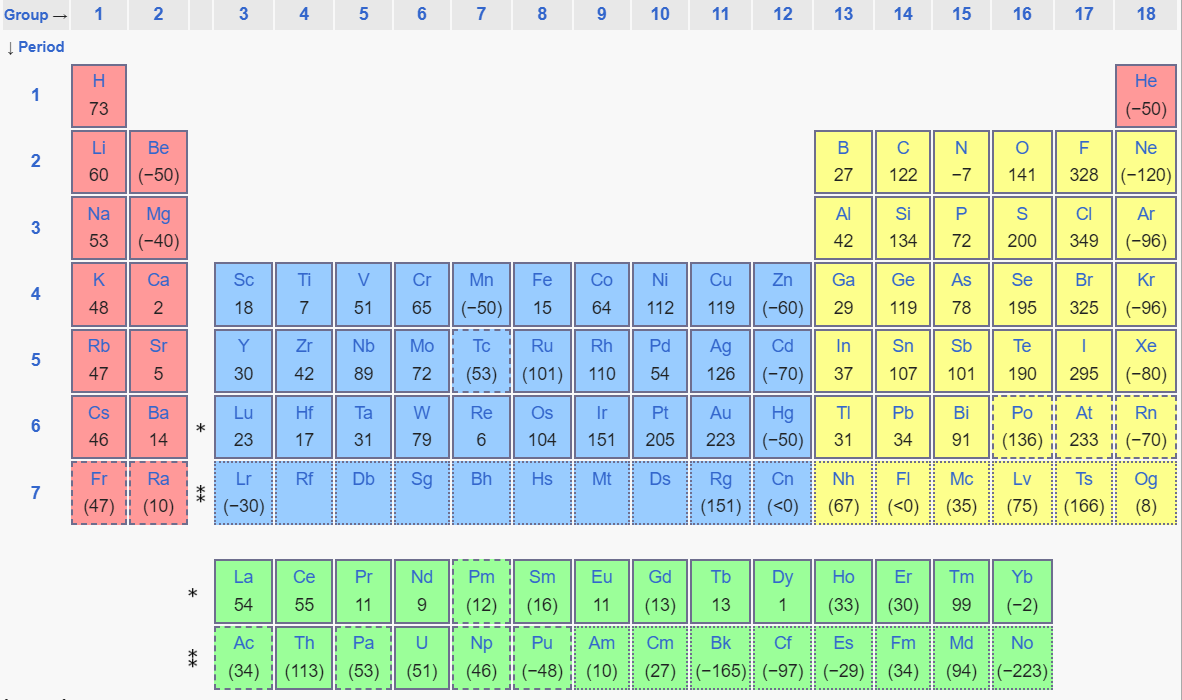
\includegraphics[width=\textwidth]{ukok.png}
    \caption{Wartości powinowactwa elektronowego}
    \label{fig:ukok}
\end{figure}
\textbf{Elektroujemność} - zdolność atomu danego pierwiastka do przyciągania elektronu. Największą elektroujemność przypisuje się fluorowi (4.0). W miarę wzrostu ładunku jądra elektroujemność rośnie (pierwiastki pierwszej i drugiej grupy mają małe wartości elektroujemności, 0,7-1,5, natomiast tlenowce i fluorowce charakteryzują się wartościami elektroujemności, w granicach 2-4). W obrębie grupy elektroujemność maleje ze wzrostem rozmiarów atomów.\\

\textbf{Potencjał standardowy}

Elektrony mogą samorzutnie przemieszczać się z punktu o niższym potencjale elektrycznym do punktu o potencjale wyższym. W ogniwie więc elektrony będą przemieszczać się od elektrody o potencjale niższym do elektrody o potencjale wyższym. 

Przyjmuje się, że metal ulegający redukcji ma wyższy potencjał niż metal ulegający utlenieniu. Im metal chętniej ulega reakcji utleniania (np. $\text{Zn}\rightarrow \text{Zn}^{2+}+2\text{e}$), tym niższy potencjał. W rezultacie najwyższym potencjał mają metale szlachetne, które najtrudniej ulegają utlenieniu, natomiast najmniej szlachetne, czyli łatwo ulegające utlenienia, mają potencjały najniższe. 

Pojęcie potencjału w sposób ścisły nie odnosimy do samego metalu, ale do układu metal wraz z roztworem jonu metalu, w którym jest zanurzony. Układ taki to półogniwo metaliczne. Z pomiarów możemy uzyskać tylko różnicę potencjałów tych dwóch elektrod, a nie wartość potencjału tylko dla jednej elektrody, dlatego potencjał przypisuje się elektrodzie na zasadzie konwencji, czyli względem elektrody wodorowej, której potencjał przyjmuje się za równy zeru.

Potencjał elektrody zależeć będzie od stężenia kationów metalu w roztworze, dlatego używa się \textbf{potencjału standardowego}, czyli potencjału półogniwa dla stężenia jonów metalu wynoszącego 1 mol/dm$^3$.

Metal o najniższej wartości potencjału standardowego to lit, bo jest najsilniejszym reduktorem. Najsłabszym reduktorem jest złoto, które najtrudniej ulega utlenieniu.

Na podstawie wartości potencjałów standardowych można przewidzieć kierunek reakcji redoks. Skoro metal o niższym potencjale standardowym łatwiej ulega utlenieniu, to metal ten będzie wypierał z roztworu metal o wyższym potencjale standardowym. Np.:
\begin{equation*}
    \text{Pb}+2\text{Ag}^+\rightarrow\text{Pb}^{2+}+2\text{Ag}
\end{equation*}

\begin{figure}[H]
    \centering
    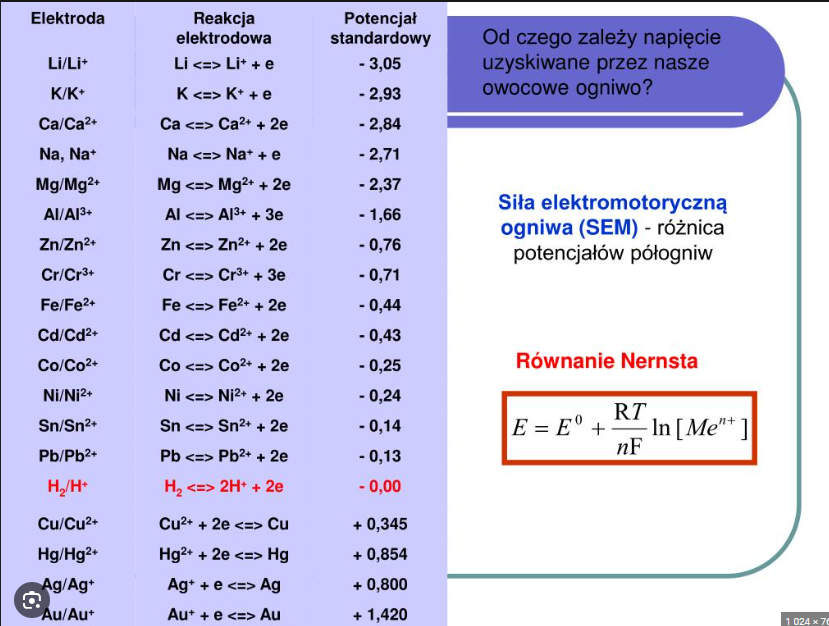
\includegraphics[width=\textwidth]{images/potencjaly_standardowe.png}
\end{figure}

Wypieranie się metali. Film: \url{https://www.youtube.com/watch?v=N0sznaoFaGI}

Gdy dwa atomy tworzą wiązanie chemiczne, atom o wyższej elektroujemności będzie miał większy udział w gęstości elektronowej. Ta różnica w elektroujemności między dwoma atomami określa charakter wiązania. Jeśli różnica elektroujemności jest duża (większa niż 1,7), wiązanie ma charakter jonowy. Wynika to z faktu, że atom o wyższej elektroujemności będzie przyciągał elektrony tak silnie, że zasadniczo zabierze elektron z drugiego atomu, co spowoduje utworzenie jonów. Na przykład w chlorku sodu (NaCl) sód (Na) ma elektroujemność 0,93, a chlor (Cl) ma elektroujemność 3,16. Różnica wynosi 2,23, czyli więcej niż 1,7, więc wiązanie jest jonowe. \\
Jeśli różnica elektroujemności jest niewielka (mniejsza niż 0,5), wiązanie jest kowalencyjne. Oznacza to, że elektrony są dzielone mniej więcej po równo między dwa atomy. Na przykład w cząsteczce chloru gazowego (Cl$_2$) oba atomy chloru mają taką samą elektroujemność, więc różnica wynosi zero. Oznacza to, że wiązanie jest idealnie kowalencyjne.\\
Jeśli różnica elektroujemności jest pośrednia (między 0,5 a 1,7), wiązanie jest polarne kowalencyjne. W polarnym wiązaniu kowalencyjnym elektrony są współdzielone, ale nie po równo. Atom o wyższej elektroujemności będzie miał nieco większy udział w gęstości elektronowej, co spowoduje częściowy ładunek ujemny ($\delta -$), podczas gdy drugi atom będzie miał częściowy ładunek dodatni ($\delta +$). Przykładem tego jest woda (H$_2$O), w której atom tlenu jest bardziej elektroujemny niż atomy wodoru, co skutkuje polarnym wiązaniem kowalencyjnym.

\section{Wiązania chemiczne: definicja, klasyfikacja, przykłady, uszeregowanie oddziaływań chemicznych według wzrastającej energii wiązania}

Wiązanie chemiczne łączy atomy. Powstaje, jeżeli energia utowrzonego związku jest mniejsza od sumy energii oddzielnych atomów.

\textbf{Klasyfikacja wiązań (uszeregowane według wzrastającej energii wiązania:}
\begin{itemize}
    \item \textbf{Wiązanie jonowe} -- jest wynikiem przyciągania się przeciwnych ładunków kationów i anionów (żadne wiązanie nie jest jednak czysto jonowe). Łączy pierwiastki metaliczne, zwłaszcza metali bloku $s$ (które mają niską energię jonizacji, stosunkowo łatwo oddają swoje elektrony walencyjne i tworzą kationy), z niemetalami, które mają duże powinowactwo elektronowe (dużą zdolność do przyłączania elektronu). Związki jonowe są zbudowane z kationów i anionów, które tworzą uporządkowany układ przestrzenny -- kryształy. Występuje silne przyciąganie się przeciwnie naładowanych jonów, substancje jonowe są kruche i mają wysokie temperatury topnienia i wrzenia (trzeba dużo energii, żeby przemieścić jony względem siebie, są więźniami sieci krystalicznej). Substancje jonowe można rozdzielić, rozpuszczając je w wodzie. Tworzą wtedy roztwory elektrolitów (jonowe). Gdy powstaje wiązanie jonowe, jeden atom traci elektrony, a drugi przyłącza je, w wyniku czego obydwa atomy uzyskują konfigurację gazu szlachetnego. Przykład: wiązanie w NaCl.
    \item \textbf{Wiązanie kowalencyjne} -- tworzone przez parę elektronów uwspólnioną przez dwa atomy, których energie jonizacji są zbyt wysokie, aby tworzyć kationy. Uwspólniają elektrony, by uzyskać konfigurację gazu szlachetnego. W ten sposób wiążą się niemetale. Żaden z atomów nie musi całkowicie uwolnić elektronu, nie jest więc konieczne dostarczenie mu pełnej energii jonizacji. Uwspólnienie elektronu odpowiada jego \textit{częściowemu} uwspólnieniu, potrzeba więc mniej energii.
\end{itemize}
Są to graniczne przypadki wiązania chemicznego. Wiązanie kowalencyjne ma pewien charakter jonowy, jeżeli jeden z połączonych tym wiązaniem atomów silniej przyciąga elektrony niż drugi. Jeżeli ich elektroujemność jest jednakowa (pryzkład: H$_2$), mają one równe udziały w uwspólnionych elektronach. Jeżeli elektroujemności te znacznie się różnią, elektrony znajdują się przy bardziej elektroujemnym atomie. Atom ten upodabnia się więc do anionu, a drugi do kationu. Wiązanie takie ma wtedy charakter jonowy i nazywane jest wiązaniem kowalencyjnym spolaryzowanym. Przykładem może być wiązanie w HCl lub w H$_2$O. Wiązanie kowalencyjne spolaryzowane ma charakter dipola elektrycznego.
\begin{itemize}
\item \textbf{Wiązanie metaliczne} - rodzaj wiązania chemicznego, które powstaje w wyniku elektrostatycznej siły przyciągania pomiędzy elektronami przewodzącymi (w postaci chmury elektronowej zdelokalizowanych elektronów) a dodatnio naładowanymi jonami metali. Można to opisać jako „uwspólnione” elektronów w strukturze dodatnio naładowanych jonów (kationów). Elektrony zostają „uwspólnione” w całym krysztale. Są zdelokalizowane i tworzą izotropowy rozkład ładunku. Wiązania nie są ukierunkowane. Jony dodatnie są zanurzone w morzu gęstości ładunku ujemnego. Krystalizują w strukturach najgęstszego upakowania. Przykładem może być wiązanie metaliczne w krysztale sodu.
\end{itemize}

Wiązanie metaliczne powstaje w wyniku utraty elektronów przez atomy metalu. W wyniku przyciągania pomiędzy tą chmurą elektronów i kationów tworzy się wiązanie metaliczne. Natomiast wiązanie kowalencyjne powstaje w wyniku nakładania się orbitali atomowych mających sparowane elektrony. Siła wiązania zależy od stopnia nakładania się i nakładania się rodzaju orbitali, dlatego wiązanie metaliczne jest słabsze od kowalencyjnego.
\begin{itemize}
\item \textbf{Wiązanie van der Vaalsa} -- występują pomiędzy cząsteczkami bez trwałego momentu dipolowego (zależy od definicji, może też obejmować cząsteczki o trwałym momencie dipolowym - warto pamiętać o wiązaniach wodorowych, które mogą być, lub nie, uznane za oddziaływania van der Vaalsa; technicznie rzecz biorąc nie jest to wiązanie, lecz jedynie oddziaływanie - M. Masz rację. IUPAC mówi to samo a więc tak musi być, oddziaływania van der Waalsa obejmują:  dipole–dipole, dipole-induced dipole and London (instantaneous induced dipole-induced dipole) forces. Więc to co ja napisałam to oddziaływania Londona - W). Siły te powstają na skutek płynności chmur elektronowych poszczególnych pierwiastków, która doprowadza do powstania chwilowego momentu dipolowego, a tym samym chwilowego odpychania lub przyciągania się sąsiednich cząsteczek. Tworzone przez atomy o zamkniętych powłokach. Przykładem są kryształy gazów szlachetnych, np. argonu, w niskich temperaturach. 
\end{itemize}
\section{Podstawy elektrochemii w wodnych roztworach elektrolitów na przykładzie
woltamperometrii cyklicznej.}

W metodzie woltamperometrii cyklicznej do elektrody roboczej przykłada się piłokształtny potencjał i mierzy zmiany natężenia prądu. Kształt krzywej woltamperometrycznej przypomina z początku krzywą otrzymaną przy liniowym przemiataniu potencjału, lecz gdy bezwzględna wartość potencjału zaczyna maleć, następuje gwałtowna zmiana prądu wywołana przez znaczne nagromadzenie w pobliżu elektrody utlenianych cząsteczek, które zostały utworzone w trakcie przemiatania redukcyjnego. Następnie, gdy potencjał staje się znowu zbliżony do potencjału potrzebnego do utlenienia formy zredukowanej, pojawia się znaczny prąd anodowy. Po zakończeniu utleniania prąd ten powraca do wartości zerowej.\\
\url{https://www.youtube.com/watch?v=cz67DnyS9-w}

\section{Potencjometria: podstawy metody. Elektrody pierwszego i drugiego rodzaju, ich zastosowanie w potencjometrii. Elektroda szklana, wodorowa i chlorosrebrowa. Zależność potencjału elektrody wskaźnikowej od stężenia oznaczanych jonów.}

\textbf{Reakcje utleniania i redukcji} (redoks) -- w reakcjach takich następuje przeniesienie elektronów między reagentami. Substancję, która oddaje elektrony nazywa reduktorem, a substancję, która przyjmuje elektrony -- utleniaczem.

Reakcja utleniania -- reduktor przechodzi w postać uboższą w elektrony:
\begin{equation*}
    \text{Red}_1 \rightarrow \text{Utl}_1+n_1e
\end{equation*}

Reakcja redukcji -- utleniacz pobiera elektrony i redukuje się:
\begin{equation*}
    \text{Utl}_2 +n_2e \rightarrow \text{Red}_2
\end{equation*}

\textbf{Potencjometria} -– zespół pomiarowych metod elektrochemicznych, polegających na wyznaczaniu wartości potencjału elektrody wskaźnikowej (roboczej, której potencjał zależy od oznaczanego jonu) względem elektrody porównawczej (odniesienia, której potencjał jest stały) w funkcji logarytmu stężenia jonów elektroaktywnych. Pomiary są wykonywane w warunkach bezprądowych (w stanie równowagi), dzięki czemu może być stosowane równanie Nernsta:
\begin{figure}[H]
    \centering
    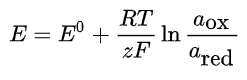
\includegraphics[width=0.2\textwidth]{images/nernst.png}
\end{figure}

Aktywność $i$-tego jonu dana jest wzorem:
\begin{equation*}
    a_i=f_iC_i
\end{equation*}
gdzie $f_i$ to współczynnik aktywności.

Potencjometria to pomiar SEM, czyli siły elektromotorycznej w warunkach bezprądowych (obwód otwarty). Jest to technika równowagowa, która pozwala zmierzyć aktywność jonów (nie stężenie). Wykorzystuje się, że potencjał ogniwa to liniowa funkcja logarytmu aktywności. Jest to pomiar siły elektromotorycznej (SEM) ogniwa złożonego z dwu elektrod (wskaźnikowej i porównawczej) zanurzonych do badanego roztworu. Zasada potencjometrii opiera się na wykorzystaniu faktu, iż potencjał elektryczny ($E$) odpowiednio dobranej elektrody zależy od składu roztworu, w którym jest ona zanurzona.

Siła elektromotoryczna ogniwa (SEM) jest to napięcie między półogniwami niepracującego ogniwa galwanicznego.
Jednostką SEM jest wolt [V]. Siłę elektromotoryczną ogniwa oblicza się, odejmując od potencjału katody potencjał anody. Warto pamiętać, że potencjał katody jest większy od potencjału anody. Napięcie pomiędzy dwoma półogniwami jest największe właśnie wtedy, gdy ogniwo nie pracuje.

Przykładem potencjometrii jest miareczkowanie redoks, które polega na pomiarze różnicy potencjałów między elektrodą wskaźnikową i porównawczą po dodaniu każdej porcji tiranta, np.:
\begin{equation*}
    \text{C}^{4+}+\text{Fe}^{2+}+e\longleftrightarrow\text{Fe}^{3+}+\text{Ce}^{3+}+e
\end{equation*}
\begin{figure}[H]
    \centering
    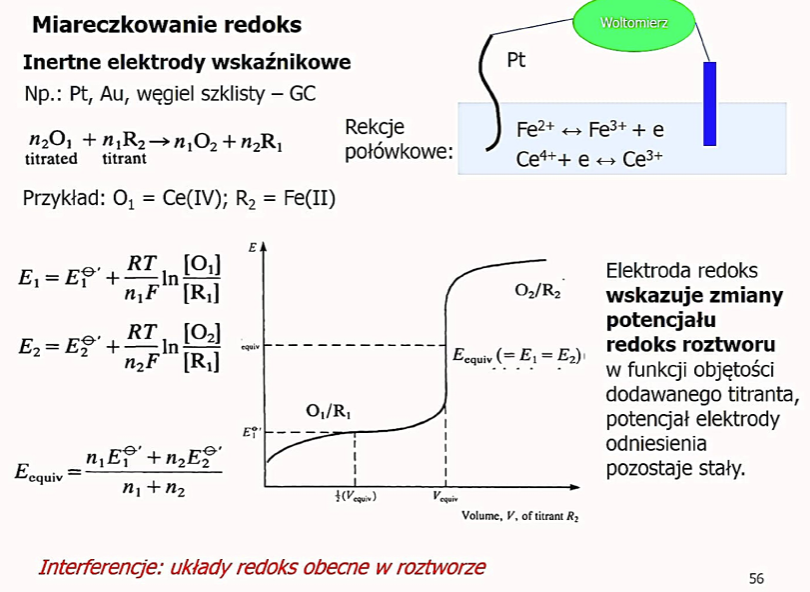
\includegraphics[width=0.8\textwidth]{images/miareczkowanie.png}
\end{figure}
 
W pierwszej części wykresu następuje redukcja oznaczanego jonu Ce$^{4+}$: $\text{Ce}^{4+}+e \rightarrow \text{Ce}^{3+}$ i SEM zależy od stosunku $[\text{Ce}^{4+}]/[\text{Ce}^{3+}]$. SEM zmienia się nieznacznie w zależności od tych stężeń. W punkcie \textit{equiv} wszystkie $\text{Ce}^{4+}$ przereagowały i zostało tylko $\text{Ce}^{3+}$, czyli następuje duża zmiana SEM przez zmianę aktywnego jonu. Potencjał elektrody wskaźnikowej zależy wówczas od stosunku $[\text{Fe}^{3+}]/[\text{Ce}^{3+}]$. Po tym punkcie obserwujemy niewielkie zmiany SEM.

\textbf{Ogniwo} to urządzenie bezpośrednio zamieniające energię chemiczną na energię elektryczną prądu stałego.

\textbf{Ogniwo nieodwracalne} (ogniwo pierwotne) ogniwo galwaniczne, w którym reakcje chemiczne przebiegają
w sposób nieodwracalny (tylko w jednym kierunku).

\textbf{Ogniwo odwracalne} (ogniwo wtórne) ogniwo galwaniczne, w którym reakcje chemiczne przebiegają w sposób
odwracalny, tzn. możliwa jest regeneracja materiału elektrod, w wyniku przepuszczania przez układ prądu stałego z zewnętrznego źródła; ogniwami galwanicznymi odwracalnymi są akumulatory elektryczne.

\textbf{Elektroda pierwszego rodzaju} –- elektroda odwracalna (równowagowa) z jedną granicą faz, na której zachodzi szybka, odwracalna reakcja potencjałotwórcza -– reakcja utleniania lub redukcji. Potencjał powstaje na granicy między metalem i elektrolitem, przy czym metal jest jednym z reagentów lub pełni tylko funkcję przenośnika elektronów między reagentami znajdującymi się w otoczeniu. Przykładem może być elektroda miedziana i cynkowa w ogniwie elektrochemicznym (Cu|Cu$^{2+}$, Zn|Zn$^{2+}$), które ulegają reakcjom utlenienia i redukcji:
\begin{gather*}
    \text{Zn} \rightarrow \text{Zn}^{2+}+2e\\
    \text{Cu}^{2+} +2e \rightarrow \text{Cu}
\end{gather*}
\begin{figure}[H]
    \centering
    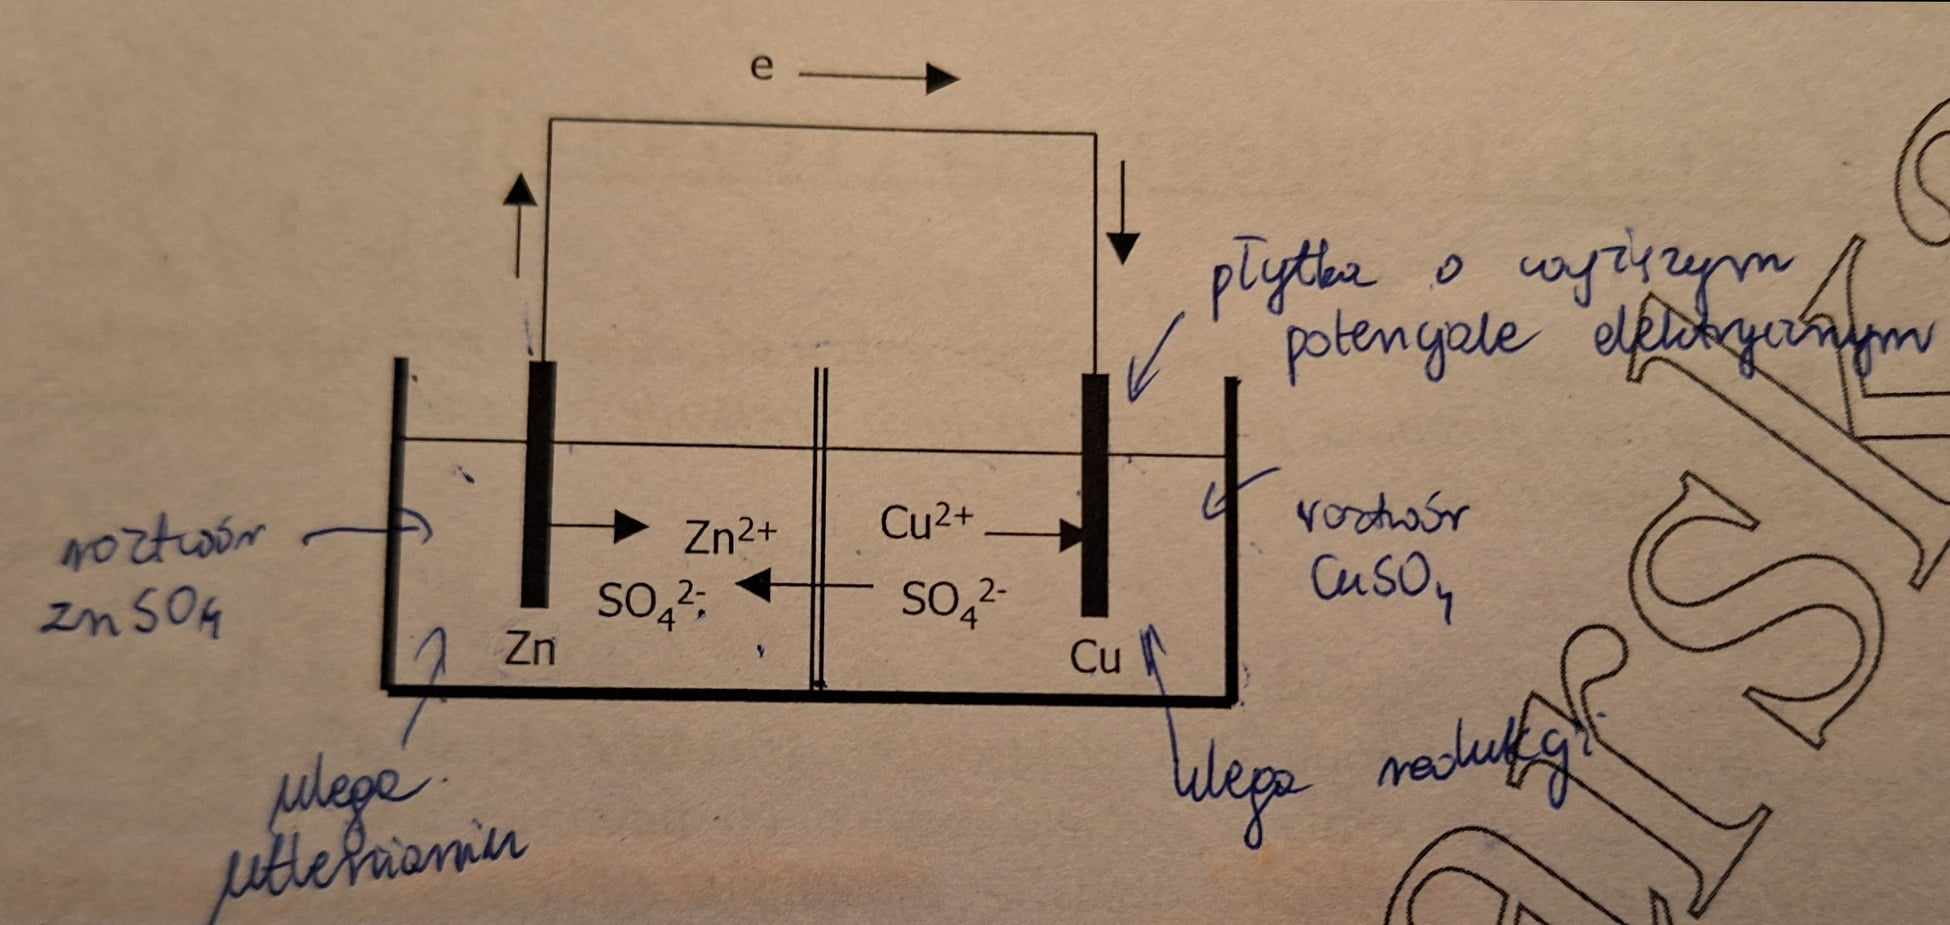
\includegraphics[width=0.7\textwidth]{images/ogniwo.jpg}
    \caption{Schemat ogniwa miedziano-cynkowego}
\end{figure}

\begin{figure}[H]
    \centering
    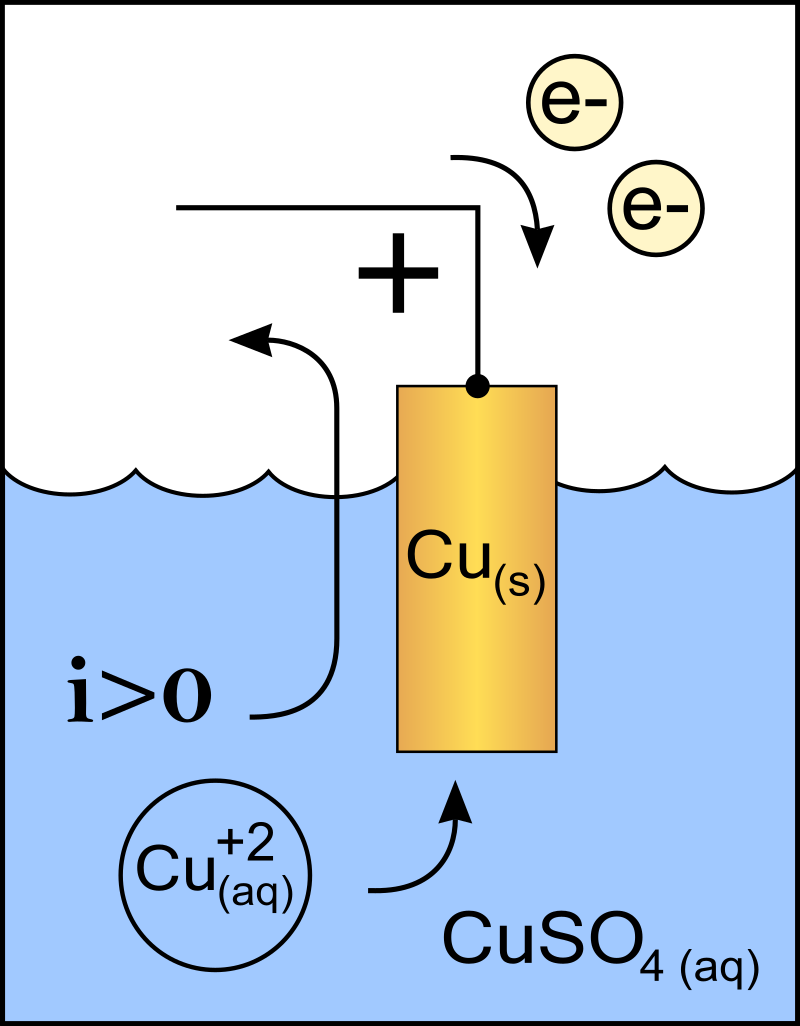
\includegraphics[width=0.2\textwidth]{images/elektroda_miedziana.png}
    \caption{Schemat elektrody miedzianej}
\end{figure}

\textbf{Elektrody drugiego rodzaju} –- odwracalne względem kationu lub anionu.
Np. elektroda srebrowa Ag|Ag$^+$, wodorowa Pt|H$_2$(g)|H$^+$ lub chlorowa Pt|Cl$_2$(g)|Cl$^-$.

\begin{figure}[H]
    \centering
    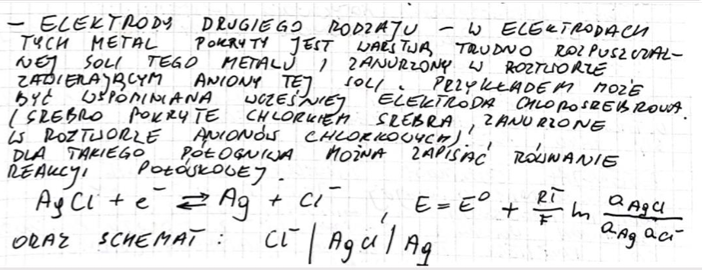
\includegraphics[width=0.7\textwidth]{images/elektrody2.png}
\end{figure}

\textbf{Elektrody szklane} -- elektroda wskaźnikowa, czyli taka, która reaguje zmianą potencjału na obecność badanych jonów w roztworze. Potencjał takiej elektrody zależy zatem od aktywności roztworu, w jakim się znajduje. Elektroda szklana składa się z rurki szklanej zakończonej cienkościenną banieczką ze szkła elektrodowego. Wewnątrz rurki znajduje się elektroda wewnętrzna (wyprowadzająca), którą jest elektroda chlorosrebrowa (Ag/AgCl) zanurzona w roztworze wewnętrznym, o stałej aktywności jonów, w stosuku których jest ona odwracalna. W przypadku elektrod szklanych do pomiaru pH roztworem wewnętrznym jest 0,1 mol$\cdot$dm$^{-3}$ HCl (0,1M HCl).

\begin{figure}[H]
    \centering
    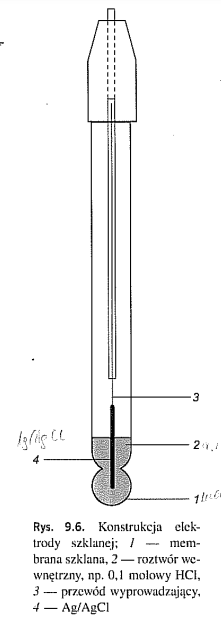
\includegraphics[width=0.25\textwidth]{images/elektroda_szklana.png}
\end{figure}

\begin{figure}[H]
    \centering
    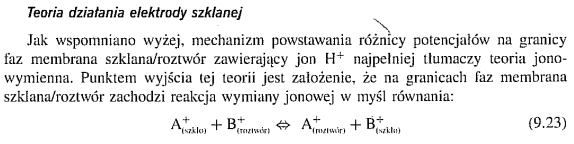
\includegraphics[width=0.7\textwidth]{images/szk1.png}
\end{figure}
\begin{figure}[H]
    \centering
    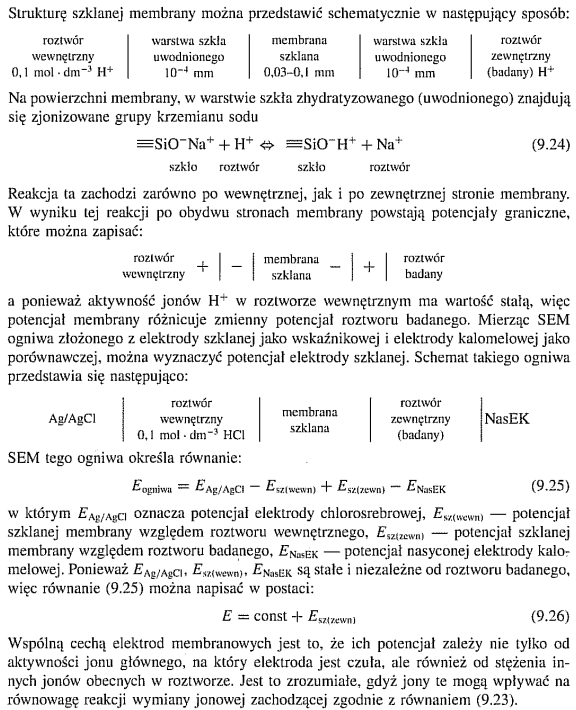
\includegraphics[width=0.7\textwidth]{images/szk2.png}
\end{figure}

\textbf{Elektroda wodorowa} -- półogniwo, którego potencjał jest określony równowagą reakcji:
\begin{center}
H$_2$ $\longleftrightarrow$ 2H$^+$ + 2$e$.
\end{center}
Elektroda ta składa się z blaszki platynowej, pokrytej czernią platynową, zanurzonej w roztworze jonów wodorowych, omywanej gazowym wodorem; przy stałym ciśnieniu gazowego wodoru potencjał e.w. zależy od aktywności jonów wodorowych w roztworze, wobec czego może służyć do jej wyznaczenia (a więc do wyznaczenia pH). Potencjał standardowej e.w., dla której aktywność jonów wodorowych w roztworze (np. HCl) wynosi 1, natomiast ciśnienie gazowego wodoru — 101 325 Pa (1 atm), przyjęto jako wzorzec pierwotny, względem którego mierzone są potencjały innych elektrod; potencjał standardowej e.w. przyjęto w dowolnej temp. jako równy 0,00 V. W praktyce elektrochem. posługiwanie się e.w. jest niewygodne i jako wzorce wtórne stosowane są inne elektrody odniesienia.

Z pomiarów przeprowadzanych dla ogniwa można uzyskać jedynie różnicę potencjałów dwóch półogniw, nie ma możliwości wyznaczenia wartości potencjału tylko dla jednej elektrody. Elektrodzie można przypisać określony potencjał tylko na zasadzie konwencji, wyrażając jej potencjał względem inne elektrody, który potencjał przyjmuje się równy zeru. Elektrodą taką jest standardowa elektroda wodorowa. 
\begin{figure}[H]
    \centering
    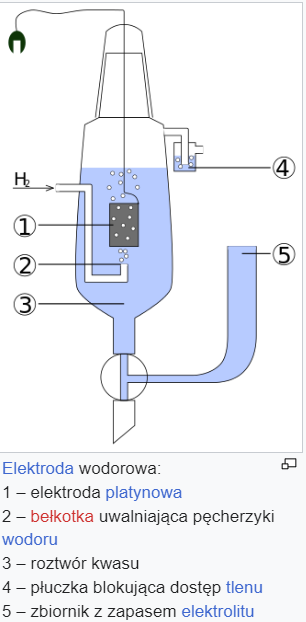
\includegraphics[width=0.25\textwidth]{images/wodorowa.png}
\end{figure}

\textbf{Elektroda chlorosrebrowa}
\begin{figure}[H]
    \centering
    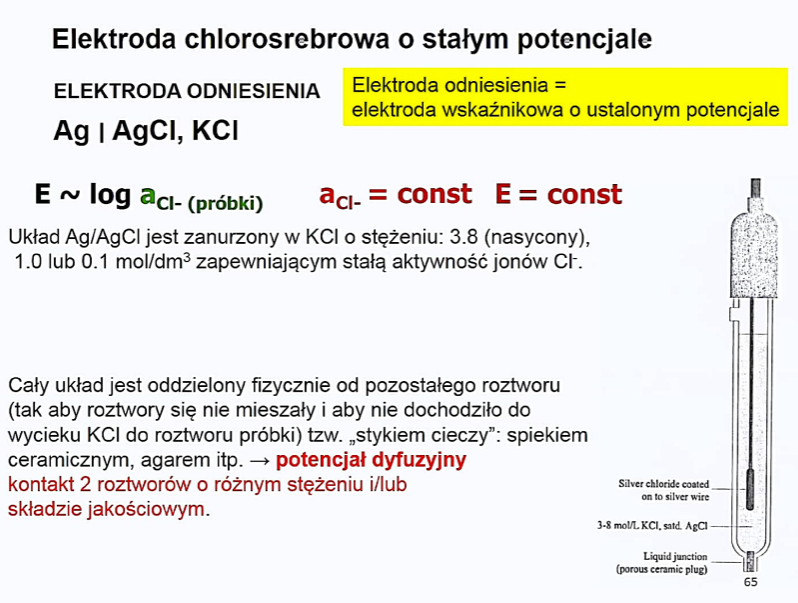
\includegraphics[width=0.8\textwidth]{images/chlorosreborwa1.png}
\end{figure}

\begin{figure}[H]
    \centering
    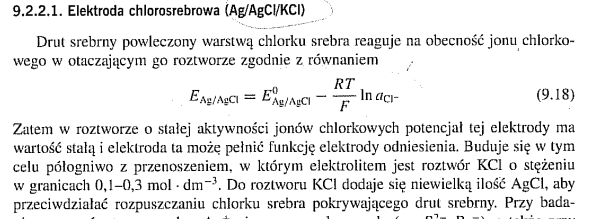
\includegraphics[width=0.8\textwidth]{images/chlorosrebrowa2.png}
\end{figure}

Elektroda chlorosrebrowa jest elektrodą drugiego rodzaju, odwracalną względem jonów chlorkowych (elektroda); jest stosowana w miareczkowaniach jako elektroda porównawcza.

\section{Spin jądra atomowego i elektronu. Wpływ spinów jądrowych na symetrię funkcji falowej cząsteczek. Związek spinu ze statystyką, symetria permutacyjna funkcji falowej dla układu wielu ciał.}
Spin to wewnętrzny moment pędu cząstki. Elektron może mieć spin 1/2 lub -1/2, co odpowiada rzutowi wektora spinu na oś z. Spin określa spinowa liczba kwantowa.

Spin jądra:
\begin{itemize}
    \item całkowity -- jądro jest bozonem (składa się z parzystej liczby nukleonów).
    \item ułamkowy -- jądro jest fermionem (składa się z nieparzystej liczby nukleonów).
\end{itemize}

Rozważmy permutacje współrzędnych par cząstek identycznych (o takim samym ładunku i spinie):
\begin{equation}
\label{permutacja}
    (\mathbf{r}_i, n_{s,i},...,\mathbf{r_j}, n_{s,j}) \rightarrow (\mathbf{r}_j, n_{s,j},...,\mathbf{r_i}, n_{s,i})
\end{equation}
Hamiltonian układu wielu cząstek posiada symetrię permutacyjną i to znajduje odzwierciedlenie we właściwościach jego funkcji własnych opisanych poniżej.


Jeżeli cząstki są fermionami, czyli mają spin połówkowy, to funkcja falowa układu N cząstek identycznych musi być \textbf{antysymetryczna} ze względu na permutacje (\ref{permutacja}):
\begin{equation*}
    \Psi(1, 2, ...,i,...,j,...,N) =-\Psi((1, 2, ...,j,...,i,...,N) )
\end{equation*}
Wynika to z zakazu Pauliego, który głosi, ze dwa fermiony nie mogą równocześnie zajmować tego samego stanu kwantowego. Funkcja falowa opisująca układ identycznych fermionów jest antysymetryczna.
Jeżeli dwa fermiony o tym samym spinie będą przebywać w jednym stanie, czyli $j=i$, to:
\begin{equation*}
    \Psi(1, 2, ...,i,...,i,...,N) =-\Psi((1, 2, ...,i,...,i,...,N))=0
\end{equation*}
Czyli $|\Psi^2|=0$, więc prawdopodobieństwo takiego zdarzenia jest równe 0.

Jeżeli cząstki mają spin całkowity, czyli są bozonami, to funkcja falowa układu N takich cząstek identycznych musi być symetryczna ze względu na permutacje (\ref{permutacja}) (nie zmieni ona znaku przy zamianie położeń dwóch cząstek i ich spinów):
\begin{equation*}
    \Psi(1, 2, ...,i,...,j,...,N) = \Psi((1, 2, ...,j,...,i,...,N) )
\end{equation*}
Bozony są cząstkami identycznymi i ich przestawienie nie prowadzi do innego stanu $n$-cząstkowego.


\section{Ogólna charakterystyka najważniejszych związków nieorganicznych: tlenków, wodorotlenków, kwasów, wodorków, soli oraz powiązanie ich właściwości z położeniem pierwiastków w układzie okresowym.}

Wszystkie pierwiastki grup głównych, z wyjątkiem gazów szlachetnych tworzą binarne \textbf{wodorki}, w których można szukać właściwości okresowych. Wzory binarnych wodorków są bezpośrednio związane z numerem grupy i ujawniają typowe właściwości pierwiastków. Na przykład węgiel tworzy CH$_4$, azot - NH$_3$, tlen - H$_2$O, a fluor - HF. Charakter konkretnego wodorku binarnego jest związany z właściwościami jego pierwiastka macierzystego. 

Silnie elektrododatnie pierwiastki metaliczne tworzą związki jonowe (\textbf{wodorki jonowe}), w których wodór występuje jako jon wodorkowy H$^-$ i ma stopień utlenienia -1. Są to wodorki typu soli (solopodobne), tworzone przez wszystkie pierwiastki bloku $s$ z wyjątkiem berylu. Powstają zwykle w wyniku ogrzewania metalu w wodorze. Są to białe wysokotopliwe substancje, przypominające strukturą krystaliczną odpowiednie halogenki. Na przykład wodorki litowców mają strukturę soli kuchennej. Rozkładają się w reakcji z wodą:
\begin{equation*}
    \text{LiH}+\text{H}_2\text{O}\rightarrow \text{LiOH}+\text{H}_2\uparrow 
\end{equation*}



Wodorki metaliczne to czarne, przewodzące elektryczność proszki. Powstają przez ogrzewanie pewnych metali bloku $d$ w wodorze. Rozkładają się z wydzieleniem H$_2$ (możliwość magazynowania wodoru). Atomy wodoru lokują się w sieci krystalicznej metalu w połączeniach międzywęzłowych pomiędzy atomami, przez co nie mają konkretnego wzoru. Pallad jest metalem o dużej zdolności magazynowania wodoru. Charakter oddziaływań jest bardziej fizyczny niż chemiczny.

Niemetale tworzą \textbf{wodorki kowalencyjne}, złożone z oddzielnych cząsteczek. Wodorki z pierwiastkami o większej elektroujemności. Związki te mają niskie temperatury topnienia i są lotne. Większość tych wodorków stanowią gazy (amoniak, halogenki wodoru - HF, HCl, HBr, HI i lżejsze węglowodory - metan, etan, eten i etyn. Do ciekłych wodorków należy woda i węglowodory (oktan, benzen). \\

Wszystkie pierwiastki grup głównych, z wyjątkiem gazów szlachetnych, reagują z tlenem. Podobnie jak wodorki, \textbf{tlenki} ujawniają okresowość właściwości pierwiastków. Na podstawie tych właściwości można zaliczać pierwiastki do metali lub niemetali: tlenki metali grup głównych są zasadowe (CaO), a niemetali - kwasowe (SiO$_2$). Mogą być również tlenki amfoteryczne (Al$_2$O$_3$). Typ wiązań zmienia się od tlenków rozpuszczalnych, jonowych (lewa strona układu okresowego, np. CaO), poprzez tlenki nierozpuszczalne, wysokotopliwe (lewa strona bloku $p$) do niskotopliwych i często gazowych tlenków cząsteczkowych (prawa strona układu okresowego). \\
Pierwiastki metaliczne o niskich energiach jonizacji tworzą zwykle tlenki jonowe. Jon tlenkowy jest mocną zasadą; tlenki większości takich metali tworzą więc w wodzie mocne zasady. Wyjątek stanowi magnez, gdyż jego tlenek, MgO, jest bardzo słabo rozpuszczalny. Nawet jednak ten tlenek reaguje z kwasami, zalicza się go więc do tlenków zasadowych. Pierwiastki o średnich energiach jonizacji (beryl, glin, większość półmetali) tworzą tlenki amfoteryczne. Tlenki te nie reagują z wodą, lecz wiele z nich rozpuszcza się w roztworach kwasowych i zasadowych. \\
Wiele tlenków niemetali to gazowe związki cząsteczkowe; ich przykłady to CO$_2$, NO i SO$_3$. Większość zachowuje się jak kwasy Lewisa, gdyż elektroujemne atomy tlenu odciągają elektrony od atomu centralnego, powodując, że staje się on akceptorem pary elektronowej. Na przykład ditlenek węgla może reagować z tlenkami metali, gdyż jon tlenkowy jest mocną zasadą Lewisa. \\
Wiele tlenków niemetali tworzy w wodzie roztwory kwasowe; HNO$_3$ i H$_2$SO$_4$ pochodzą od tlenków kwasowych, nazywanych w związku z tym bezwodnikami kwasowymi. Bezwodnik kwasowy to tlenek powstający z kwasu przez usunięcie wody; uwodniony bezwodnik tworzy kwas. Formalny bezwodnik kwasu to cząsteczka otrzymana przez skreślenie pierwiastków wody z cząsteczkowego wzoru kwasu; cząsteczka ta nie reaguje jednak z wodą, tworząc kwas. Na przykład tlenek węgla stanowi formalny bezwodnik kwasu mrówkowego HCOOH, lecz tlenek ten nie tworzy z wodą kwasu. Kwasowość kwasu tlenowego zależy od elektroujemności niemetalu związanego z atomami O i jego stopnia utlenienia: im większa jest elektroujemność i im wyższy stopień utlenienia, tym mocniejszy kwas. \\
Tlenki większości półmetali i tlenki niektórych pierwiastków mniej elektrododatnich są amfoteryczne. Na przykład tlenek glinu reaguje z kwasami i wodnymi roztworami zasad. Tlenki ujawniają silne diagonalne podobieństwo między berylem a glinem, gdyż tlenek berylu jest także amfoteryczny. 



\newpage
\section{Konfiguracje elektronowe atomów i termy atomowe}
Konfiguracje elektronowe atomów opisane w pytaniu 44.

\textbf{Term atomowy} –- w mechanice kwantowej, obserwowany stan atomu, odpowiadający rzeczywistym stanom o różnej energii, charakteryzujący się określonymi wartościami liczb kwantowych. 
Jest to zespół stanów atomu, którym odpowiadałaby taka sama energia, gdyby występowały tylko oddziaływania elektrostatyczne.
\begin{figure}[H]
    \centering
    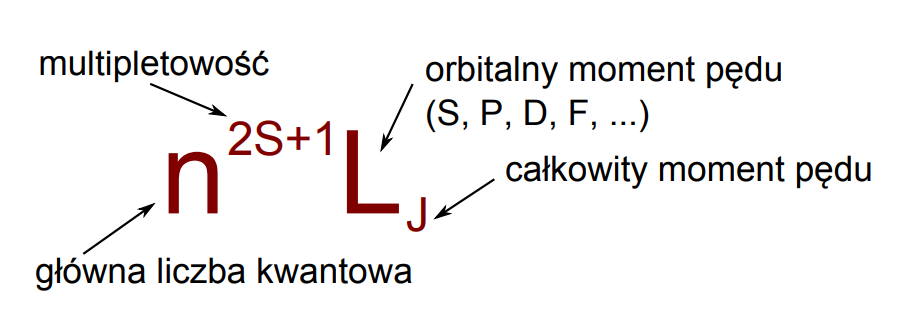
\includegraphics[width=0.5\textwidth]{images/termy.png}
\end{figure}
\begin{itemize}
    \item $L$ - liczba kwantowa, określająca kwadrat całkowitego orbitalnego momentu pędu. Oznaczenia literowe.
    \item $S$ - liczba kwantowa, określająca kwadrat całkowitego spiny.
\end{itemize}

Przykład wyznaczania termu atomowego:
\begin{figure}[H]
    \centering
    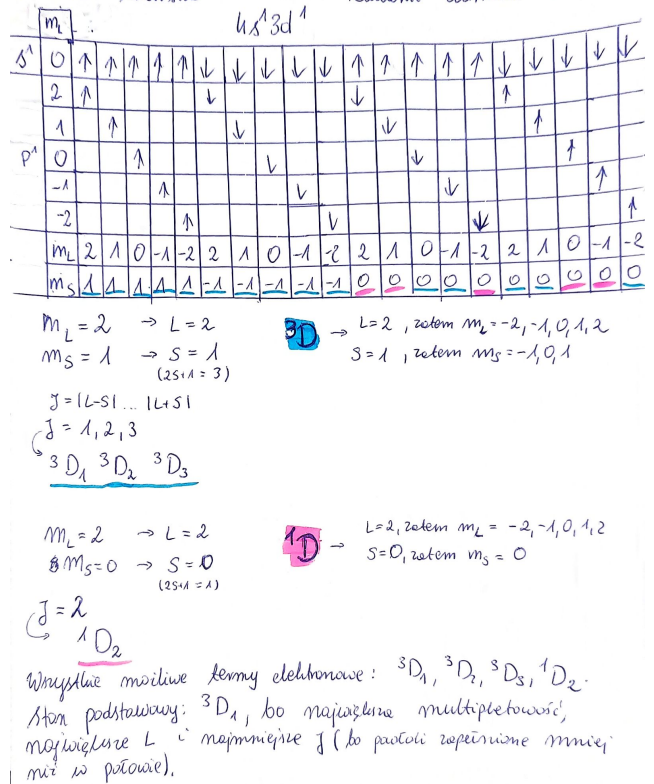
\includegraphics[width=0.8\textwidth]{images/przyklad_term.png}
\end{figure}

\section{Przybliżenie Borna-Oppenheimera. W jakich sytuacjach przybliżenie to nie działa?}
Funkcja falowa cząsteczki $\Psi_\text{mol}$, która zależna jest od współrzędnych położenia wszystkich elektronów, wszystkich jąder oraz od orientacji spinów elektronów i jader. Funkcja spełnia równanie Schrodingera:
\begin{equation*}
    \hat{H}_\text{mol}\Psi_\text{mol}=E_\text{mol}\Psi_\text{mol}
\end{equation*}
W skald operatora energii $\hat{H}_\text{mol}$ wchodzi: operator energii kinetycznej elektronów $\hat{T}_\text{el}$, operator energii kinetycznej jąder $\hat{T}_\text{jądra}$, energia odpychania kulombowskiego jąder $V_\text{jądra}$, energia odpychania kulombowskiego elektronów $V_\text{el}$, energia przyciągania elektronów przez jądra $V_\text{el-jądra}$, energia oddziaływania spinowo-orbitalnego elektronów $V_{ls}$ i inne, drugorzędne z reguły przyczynki energetyczne. Hamiltonian ten ma postać:
\begin{figure}[H]
    \centering
    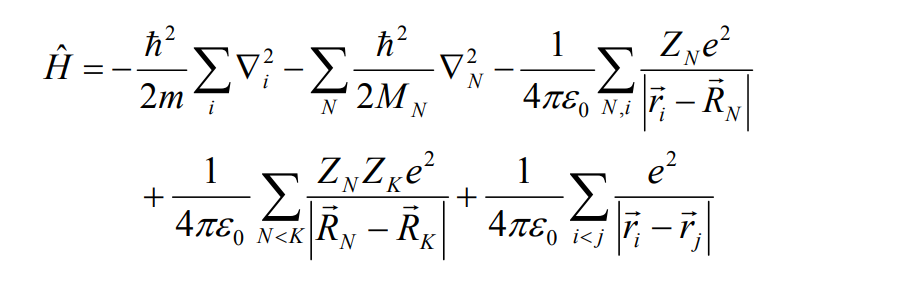
\includegraphics[width=0.6\textwidth]{images/hamiltonian cząsteczki.png}
\end{figure}
Rozwiązanie zagadnienia własnego w takim przypadku jest wyjątkowo trudne. Dlatego wprowadza się tzw. przybliżenie Borna-Oppenheimera, ewentualnie przybliżenie adiabatyczne. Ponieważ masa elektronu jest tysiące razy mniejsza od masy jader, przeto jądra, jako bardziej bezwładne, poruszają się o kilka rzędów wolniej od elektronów. Możemy przyjąć więc, że jądra zostają "zamrożone". Przybliżenie to zakłada rozdzielenie ruchu jąder i elektronów. Hamiltonian elektronowy cząsteczki nie zawiera energii kinetycznej jąder:

\begin{equation*}
    \hat{H}_\text{el}=\hat{H}_\text{mol} - \hat{T}_\text{jądra}
\end{equation*}
Wciąż zachowane są w nim człony od oddziaływania $V_\text{jądra}$ i zależą od przyjętej konfiguracji jąder.  Uproszczone zagadnienie własne energii cząsteczki ma postać:
\begin{equation*}
    \hat{H}_\text{el}\Psi_\text{el}=E_\text{el}\Psi_\text{el}
\end{equation*}
$\Psi_\text{el}$ jest zależna od położeń elektronów, ale też jąder, tylko zakładamy, że położenie to jest ustalone. Energia $E_\text{el}$ jest energią cząsteczki, ale zależy od ustalonego położenia jąder atomowych. Uwzględniając dodatkowo energię kinetyczną jąder, uzyskamy energię całkowitą cząsteczki $E_\text{mol}$. Zgodnie z przybliżeniem Borna-Oppenheimera, energia ta wynika z zagadnienia własnego:
\begin{equation*}
   [\hat{T}_\text{jądra} + E_\text{el}]\Psi_\text{jądra}=E_\text{mol}\Psi_\text{jądra}
\end{equation*}
gdzie $\Psi_\text{jądra}$ jest funkcją falową zależną wyłącznie od współrzędnych położenia jąder. Pełna funkcja falowa cząsteczki przyjmuje w przybliżeniu postać iloczynową:
\begin{equation*}
   \Psi_\text{mol} \approx \Psi_\text{el}\Psi_\text{jądra}
\end{equation*}

Przybliżenie Borna-Oppenheimera może nie działać dobrze w przypadku cząsteczek o ciężkich jądrach lub z silnym sprzężeniem między ruchami jądrowymi i elektronowymi. Może to być również problematyczne w przypadku cząsteczek o nisko położonych stanach wzbudzonych lub w przypadku reakcji obejmujących znaczące zmiany w strukturze elektronowej (tego akapitu nie jestem pewna, ale nie znalazłam nic lepszego).
\section{Przybliżenie jednoelektronowe i metoda Hartree-Focka}
Każdy elektron porusza się w uśrednionym polu wytworzonym przez pozostałe, ale niezależnie od nich
Każdy elektron ma swoją funkcję, spinorbital, zależną tylko od jego współrzędnych. 
Funkcja falowa układu $N$-elektronowego (wieloelekrtronowa funkcja falowa) to wyznacznik Slatera:
\begin{figure}[H]
    \centering
    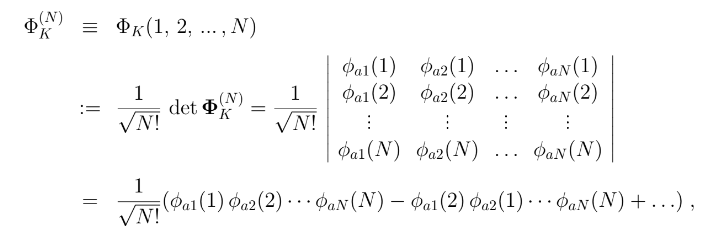
\includegraphics[width=0.6\textwidth]{images/wyznacznikSlatera.png}
\end{figure}
a ostatnia równość wskazuje, że definiowana funkcja jest sumą iloczynów spinorbitali, różniących się permutacją współrzędnych elektronów. Spinorbitale są iloczynem orbitali molekularnych i funkcji spinowych.

W metodzie Hartree-Focka dobieramy orbitale molekularne tak, aby spośród wszystkich możliwych orbitali właśnie one dawały najniższą wartość energii średniej. Oparta jest bowiem na zasadzie wariacyjnej głoszącej, iż energia stanu obliczona jako wartość oczekiwana z dowolnej funkcji falowej jest zawsze większa bądź równa energii będącej dokładnym rozwiązaniem równania Schrödingera. Funkcją próbną w metodzie wariacyjnej jest w tym przypadku wyznacznik Slatera. Tak zmieniamy postać spinorbirali, żeby zminimalizować wartość oczekiwaną.

\section{Metoda LCAO MO w kontekście struktury elektronowej cząsteczek na przykładzie cząsteczki wody. Konfiguracje elektronowe cząsteczek dwuatomowych}
W metodzie tej zakładamy, że orbitale molekularne są liniową kombinacją orbitali atomowych. Współczynnik rozwinięcia wyznaczamy metodą pola samouzgodnionego.
\begin{equation*}
    \varphi_k^{\text{MO}}=\sum_{p=1}^Nc_{kp}\chi_p^{\text{AO}}(i)
\end{equation*}
Określenie liniowe oznacza, że funkcje falowe występują tutaj w potędze pierwszej. 

Reguły liniowej kombinacji orbitali atomowych:
\begin{enumerate}
    \item Liczba tworzonych orbitali molekularnych jest \underline{równa} liczbie orbitali atomowych uwzględnionych w kombinacji. 
    \item Orbitale atomowe muszą mieć \underline{podobną} energię. 
    \item Orbitale muszą przenikać się efektywnie (atomy muszą być stosunkowo blisko siebie).
    \item Kombinacja dotyczy orbitali o tej samej symetrii (np. taka kombinacja może dotyczyć dwóch orbitali \textit{s}, dwóch orbitali \textit{p}, które nakładają się czołowo). 
\end{enumerate}

\textbf{Cząsteczka H$_2$}
Orbitale molekularne opisują wyrażenia:
\begin{gather*}
    \Psi_1=c1s_1+c1s_2\\
    \Psi_2=c1s_1-c1s_2
\end{gather*}
Cząsteczka składa się z dwóch atomów wodoru. Gdybyśmy się ulokowali w skrajnej lewej pozycji, czyli na lewo od lewego atomu wodoru, to wówczas orbital molekularny jest praktycznie równy orbitalowi atomowemu tego lewego atomu wodoru. Wpływ drugiego atomu jest pomijalny. Po przeciwnej stronie sytuacja będzie analogiczna. W miejscu, gdzie orbitale się przenikają, mamy duży udział zarówno od orbitalu 1s jednego atomu, jak i od orbitalu drugiego. Suma funkcji falowych atomowych orbitali jest większa niż wartość dla pojedynczego orbitalu atomowego. Stąd prawdopodobieństwo znalezienia elektronu w obszarze pomiędzy atomami wodoru będzie szczególnie duże. W ramach teorii orbitali molekularnych obszar ten utożsamiamy z wiązaniem chemicznym. Elektrony są jakby wciągane do obszaru pomiędzy atomami wodoru. Taki orbital molekularny nazwiemy orbitalem wiążącym ($\Psi_1$). Jeżeli mamy kombinację dwóch orbitali atomowych, to powinniśmy otrzymać dwa orbitale molekularne. Drugi przypadek jest wtedy, gdy funkcje falowe odejmują się od siebie. Wartość funkcji falowej w cząsteczce jest wyraźnie mniejsza niż wtedy, gdy atom występuje pojedynczo. W stanie opisywanym funkcją $\Psi_2$  prawdopodobieństwo znalezienia elektronu pomiędzy atomami wodoru jest bardzo małe (elektrony są wypychane z tego obszaru), co nie sprzyja tworzeniu wiązania. Ten orbital molekularny nazywamy orbitalem antywiążącym. 
\begin{figure}[H]
    \centering
    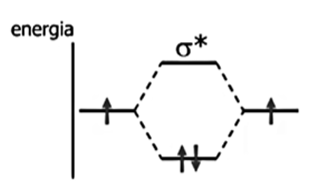
\includegraphics[width=0.4\textwidth]{images/moh2.png}
\end{figure}
Energia orbitalu wiążącego jest mniejsza niż energia wyjściowych orbitali 1s, a antywiążącego większa. Elektrony są przypisane do orbitali molekularnych zgodnie z tymi samymi zasadami, które obowiązywały dla orbitali atomowych. W przypadku H$_2$ wszystkie elektrony znalazły się na orbitalu wiążącym. Ich energia jest niższa niż w wyjściowych atomach i dlatego ta cząsteczka będzie trwała.  

\textbf{Cząsteczka He$_2$}
\begin{figure}[H]
    \centering
    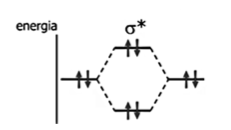
\includegraphics[width=0.4\textwidth]{images/mohe2.png}
\end{figure}
 Wiązania tutaj nie ma  i cząsteczka helu nie utworzy się, ponieważ z takiego połączenia nie byłoby zysku energetycznego.

\textbf{Cząsteczka N$_2$}
\begin{figure}[H]
    \centering
    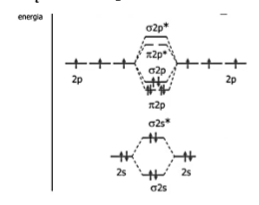
\includegraphics[width=0.6\textwidth]{images/mon2.png}
\end{figure}

\textbf{Nakładanie się orbitali na przykładzie orbitali \textit{s}}
\begin{figure}[H]
    \centering
    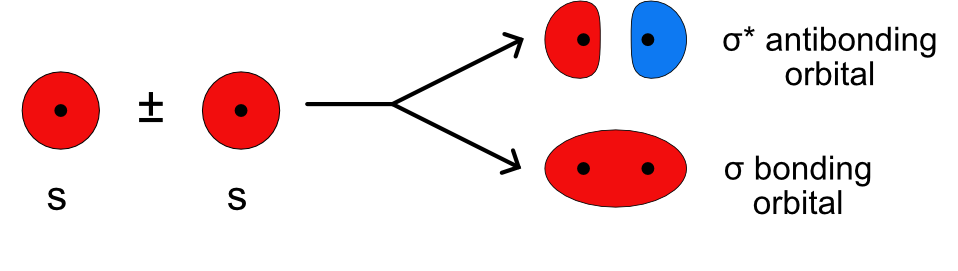
\includegraphics[width=0.6\textwidth]{images/lcao_s.png}
\end{figure}

\textbf{LCAO na przykładzie cząsteczki wody} (nie wiem, czemu każą to omawiać na podstawie tak skomplikowanej kombinacji)
\begin{figure}[H]
    \centering
    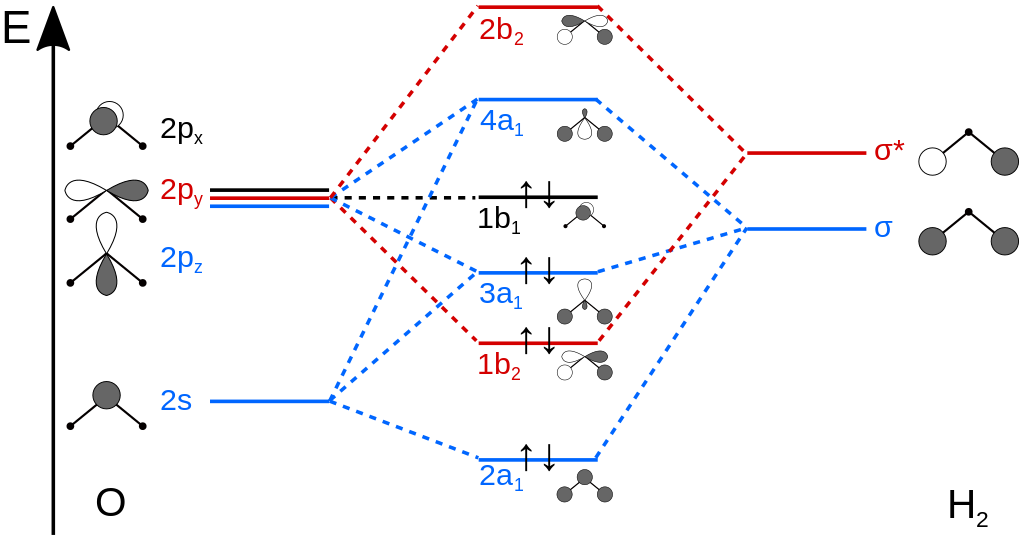
\includegraphics[width=0.6\textwidth]{images/moh2o.png}
\end{figure} 

\section{Omówić wszystkie przybliżenia, które prowadzą do podziału energii cząsteczki na wkłady: elektronowy, oscylacyjny i rotacyjny.}
\begin{figure}[H]
    \centering
    \includegraphics[width=0.8\textwidth]{images/slajd1.png}
\end{figure} 
$R_e$ -- odległość pomiędzy jądrami, dla której energia oddziaływania elektrostatycznego przyjmuje wartość minimalną (patrz pytanie 57).
\begin{figure}[H]
    \centering
    \includegraphics[width=0.8\textwidth]{images/slajd2.png}
\end{figure} 
Aby znaleźć energie elektronowe, energie kinetyczne jądra można zignorować (np. ustalić), ponieważ elektrony są znacznie szybsze niż rotacja lub wibracje.

Przy wyznaczaniu rozwiązania jądrowego ruchu oscylacyjnego zakładamy ruch, który jest czysto oscylacyjny i zakładamy, że mamy do czynienia z drganiami o małej amplitudzie, czyli $\Delta E_{el}(R)$ można rozwinąć w szereg Taylora wokół $R_e$. Jeżeli chodzi o rotacje to dla małych $\nu$ amplituda drgań jest mała i możemy założyć, że $R=R_e$. Czyli zakładamy małe drgania i powolne obroty. Wtedy można rozdzielić energię kinetyczną jąder na energię oscylacyjną i rotacyjną.
\begin{figure}[H]
    \centering
    \includegraphics[width=0.8\textwidth]{images/slajd3.png}
\end{figure}

\section{Cząsteczki dwuatomowe -- potencjał Morse'a i Lennarda-Jonesa. Przejścia optyczne w cząsteczkach dwuatomowych związane z rotacjami, oscylacjami i przejściami elektronowymi}
\begin{figure}[H]
    \centering
    \includegraphics[width=0.8\textwidth]{images/slajd4.png}
\end{figure}
Energia orbitalu antywiążącego po prostu maleje wraz ze wzrostem odległości pomiędzy atomami. Natomiast energia orbitalu wiążącego ma pewne minimum (gdy $R=R_e$). 
\begin{figure}[H]
    \centering
    \includegraphics[width=0.7\textwidth]{images/slajd5.png}
\end{figure}

\begin{figure}[H]
    \centering
    \includegraphics[width=0.7\textwidth]{images/slajd13.png}
\end{figure}

Potencjał Lennarda-Jonesa -- prosty model oscylatora anharmonicznego, który wprowadza możliwość dysocjacji wiązania i wprowadza odpychanie na małych odległościach.

\begin{equation*}
    V(r)=4\epsilon\bigg[\bigg(\frac{\sigma}{r}\bigg)^{12} - \bigg(\frac{\sigma}{r}\bigg)^{6} \bigg]
\end{equation*}

Energia oscylacji:
\begin{equation*}
    E_v=\bigg(\nu +\frac{1}{2}\bigg)\hbar\omega
\end{equation*}

Energia jądrowa stanu oscylacyjno-rotacyjnego:
\begin{equation*}
    E_n=E_v+E_J=\bigg(\nu +\frac{1}{2}\bigg)\hbar\omega+\frac{J(J+1)\hbar^2}{2\mu R_e^2}=\bigg(\nu +\frac{1}{2}\bigg)\hbar\omega+BJ(J+1)
\end{equation*}

Przejścia między poziomami w cząsteczkach:
\begin{itemize}
    \item rotacyjne -- zmianie ulega tylko $J$, poziom oscylacyjny i elektronowy pozostają bez zmian,
    \item oscylacyjno-rotacyjne -- zmianie ulegają $\nu$ i $J$, w ramach jednego poziomu elektronowego,
    \item elektronowo-oscylacyjno-rotacyjne (elektronowe) -- zmianie ulegają wszystkie liczby kwantowe $n$, $v$ i $J$.
\end{itemize}

\begin{figure}[H]
    \centering
    \includegraphics[width=0.8\textwidth]{images/slajd6.png}
\end{figure}

\begin{figure}[H]
    \centering
    \includegraphics[width=0.8\textwidth]{images/slajd7.png}
\end{figure}

\begin{figure}[H]
    \centering
    \includegraphics[width=0.8\textwidth]{images/slajd8.png}
\end{figure}

\begin{figure}[H]
    \centering
    \includegraphics[width=0.8\textwidth]{images/slajd9.png}
\end{figure}

\begin{figure}[H]
    \centering
    \includegraphics[width=0.8\textwidth]{images/slajd10.png}
\end{figure}

\begin{figure}[H]
    \centering
    \includegraphics[width=0.8\textwidth]{images/slajd11.png}
\end{figure}

\begin{figure}[H]
    \centering
    \includegraphics[width=0.8\textwidth]{images/slajd12.png}
\end{figure}

\section{Funkcje stanu. Energia swobodna, entalpia swobodna. Zależność entalpii swobodnej od temperatury i ciśnienia.}

Wartość liczbowa funkcji stanu jest określona jednoznacznie stanem termodynamicznym układu. Przyrost funkcji stanu w dowolnym procesie nie zależy od drogi procesu, a zależy tylko od początkowego i końcowego stanu układu. Do funkcji stanu zalicza się przede wszystkim same parametry stanu: ciśnienie, objętość, temperaturę, liczbę moli układu. Termodynamiczne funkcje stanu: energia wewnętrzna U, entalpia H, entropia S, energia swobodna F, entalpia swobodna G.  \\
Energia swobodna F - wielkość, która będzie równa energii stworzenia układu będącego w kontakcie z otoczeniem o stałej temperaturze T:
\begin{equation}
    F = U - T\cdot S.
\end{equation}
Jest to energia potrzebna do stworzenia układu "z niczego" minus ciepło dostarczone do układu "za darmo" z otoczenia. Jak chcemy unicestwić układ, odzyskamy energię niezbędną do jego wytworzenia, ale musimy oddać ciepło do otoczenia (które wcześniej zostało pobrane i "zużyte" na wzrost entropii układu). Energia, którą odzyskamy jest "swobodna", tzn. możemy ją dowolnie wykorzystać (w odróżnieniu od energii "nieswobodnej", która musi zostać oddana otoczeniu). \\
Entalpia swobodna G - wielkość, która będzie równa energii stworzenia układu będącego w kontakcie z otoczeniem o stałym ciśnieniu i stałej temperaturze:
\begin{equation}
    G = U + p\cdot V - T\cdot S.
\end{equation}
Jest to energia niezbędna do stworzenia układu "z niczego" plus praca wytworzenia objętości (przeciwko ciśnieniu p otoczenia), minus energia dostarczona do układu "za darmo" z otoczenia na sposób ciepła. W przypadku unicestwienia układu, entalpia swobodna oznacza energię, którą można odzyskać (stąd określenie swobodna). Jest to energia użyta do wytworzenia układu, ale po oddaniu ciepła do otoczenia (uprzednio wykorzystanego do wytworzenia entropii w układzie) i uzyskaniu pracy pochodzącej z kolapsu układu. 

\begin{equation}
    H = U + pV, \; F = U - TS \; => \; G = H - TS
\end{equation}
Nieskończenie mała zmiana entalpii równa jest różniczce zupełnej:
\begin{equation}
    dG = dH - TdS - SdT = dU + pdV + Vdp - TdS - SdT.
\end{equation}
Dla układu zamkniętego, który nie wykonuje pracy nieobjętościowej $dU$ można zastąpić równaniem: $dU = TdS - pdV$, wtedy:
\begin{equation}
    dG = -SdT + Vdp.
\end{equation}
\begin{equation}
    \left( \frac{\partial G}{\partial T}\right)_p = -S, \; \left( \frac{\partial G}{\partial p}\right)_T = V  
\end{equation}
Przy zmianie ciśnienia od $p^0$ do $p$ w stałej temperaturze:
\begin{equation}
    \Delta G = \int_{p^0}^{p}\left( \frac{\partial G}{\partial p}\right)_T dp' = \int_{p0}^{p}Vdp'
\end{equation}
Dla gazu doskonałego w stałej temperaturze:
\begin{equation}
    \Delta G = \int_{p^0}^{p}\left( \frac{nRT}{p'}\right) dp'= nRTln\left( \frac{p}{p^0}\right)
\end{equation}
\url{https://home.agh.edu.pl/~stypula/wyk5.pdf} - str 8
\section{Termochemia: definicje i znaczenie w obliczeniach termodynamicznych entalpii i molowej pojemności cieplnej. Różnice między ciepłem właściwym, pojemnością cieplną i molową pojemnością cieplną. Prawo Hessa. Zależność efektu cieplnego reakcji chemicznej od temperatury.}

Entalpia jest energią potrzebną to stworzenia układu "z niczego" plus praca wytworzenia na niego miejsca (objętości) w otoczeniu. Jeśli chcemy unicestwić układ, entalpia będzie równa energii, którą można odzyskać plus pracy kolapsu układu (zmniejszenie objętości z V do 0) wykonanej przez otoczenie. 
\begin{equation}
    H = U + pV
\end{equation}
Entalpia procesu - zmiana entalpii w związku z przebiegiem procesu:
\begin{equation}
    dH=dU+d(pV)=dQ-pdV+pdV+Vdp=dQ+Vdp
\end{equation}

Jeżeli układ nie wymienia energii w postaci pracy nieobjętościowej to entalpia układu przy stałym n jest funkcją dwóch zmiennych określających stan termiczny i mechaniczny (można przyjąć T i p): $H=f(T,p)$. Nieskończenie mała zmiana entalpii jest równa różniczce zupełnej:
\begin{equation}
    dH=\left( \frac{\partial H}{\partial T}\right)pdT + \left( \frac{\partial H}{\partial p}\right)Tdp
\end{equation}
W warunkach izobarycznych ciepło procesu jest równe zmianie entalpii $dH=Q$. Zmiana entalpii jest równa ciepłu dostarczonemu do układu pod stałym ciśnieniem (dopóki układ nie wykonuje dodatkowej pracy). Dla nieskończenie małych zmian $dH=Q=\left( \frac{\partial H}{\partial T}\right)dT$. Zamiast $Q$ możemy pisać $dQ$, gdyż w tych warunkach $Q$, jako równe $dH$, jest jednoznacznie określone przez wartości zmiennych stanu układu, stąd: 
\begin{equation}
    \left( \frac{\partial Q}{\partial T}\right)_p=\left( \frac{\partial H}{\partial T}\right)_p.
\end{equation}\\
Pochodna $\left( \frac{\partial Q}{\partial T}\right)$ wyraża ilość ciepła jaką pobiera układ przy zmianie temperatury o 1 K pod stałym ciśnieniem, czyli pojemność cieplną układu pod stałym ciśnieniem $C_p$. \\
Jeżeli układ stanowi 1 mol substancji, wielkość ta jest molową pojemnością cieplną pod stałym ciśnieniem $C_{p,m}$, jeżeli 1 g - właściwą pojemność cieplną (ciepłem właściwym). \\

Prawo Hessa: Ciepło reakcji chemicznej przebiegającej w stałej objętości lub pod stałym ciśnieniem nie zależy od tego jaką drogą przebiega reakcja, a jedynie od stanu początkowego i końcowego.

\url{https://home.agh.edu.pl/~stypula/wyk3.pdf} - Zależność ciepła reakcji od temperatury\\
Entalpia tworzenia jest to efekt cieplny towarzyszący powstawaniu 1 mola związku z pierwiastków w tych samych warunkach ciśnienia i temperatury. 
\begin{figure}[H]
    \centering
    \includegraphics[width=\textwidth]{images/kirchoff.png}
\end{figure}

\section{Potencjał chemiczny czystej substancji i substancji w mieszaninie. Potencjał chemiczny w układzie rzeczywistym -- lotność, aktywność, współczynniki aktywności. Mieszaniny cieczy -- opis termodynamiczny.}
Większość opisana w dokumencie: \url{https://drive.google.com/file/d/1eNPgWuy7RLnOJZK2k5XCGyW5qx_P11lq/view?usp=sharing}
\begin{figure}[H]
    \centering
    \includegraphics[width=\textwidth]{images/lotnosc.png}
\end{figure}

\section{Przemiany fazowe w układach jedno- i wieloskładnikowych: Diagramy fazowe substancji czystych (woda, CO$_2$). Punkt potrójny. Reguła faz Gibbsa. Prawo Raoulta. Diagramy fazowe układów dwuskładnikowych (azeotropy dodatnie i ujemne, eutektyki).}
\textbf{Przemiany fazowe} to zmian jednej fazy w inną, którym nie towarzyszą zmiany składu chemicznego.
\begin{itemize}
\item Diagramy fazowe substancji czystych (woda, CO$_2$). Punkt potrójny. Reguła faz Gibbsa: \url{https://drive.google.com/file/d/1_KqJ_fhC6W06wLaSzLwhqNtv21zfeNv8/view?usp=sharing}
\item Prawo Raoulta: \url{https://drive.google.com/file/d/1iacMwD-tiujHqGZErCphIJqyXV-g7CCR/view?usp=sharing}
\item Azeotropy dodatnie i ujemne: \url{https://drive.google.com/file/d/17jdsEeLouRUMvxeRshhOOUFHtsh-_BYS/view?usp=sharing}
\item Eutektyki: \url{https://drive.google.com/file/d/1A9J_NLKXWFAUiomTqT42HR9JU6HKYMMD/view?usp=sharing}
\end{itemize}

\section{Reakcje utleniania-redukcji, pojęcie utleniacza i reduktora. Równanie Nernsta. Współczynniki aktywności. Siła jonowa roztworu.}
Reakcje utleniania-redukcji, pojęcie utleniacza i reduktora. Równanie Nernsta. Współczynnik aktywności - opisane w pytaniu 49.
Współczynnik aktywności opisany również w skrypcie z laboratorium chemii fizycznej: \url{https://drive.google.com/file/d/1qqJeKWArWjb4wZU5pHoVOjaj3FqS8uyS/view?usp=sharing}

\begin{center}
    \textbf{Siła jonowa}
\end{center}
\begin{figure}[H]
    \centering
    \includegraphics[width=0.7\textwidth]{images/sila_jonowa.png}
\end{figure}
gdzie $c_i$ to stężenie, a $z_i$ ładunek jonu.

\section{Elektroliza: prawo Faradaya. Elektroliza wodnych roztworów różnych soli -- reakcje elektrodowe.}

\textbf{Elektroliza} – termin określający wszelkie zmiany struktury chemicznej substancji, zachodzące pod wpływem przyłożonego do niej zewnętrznego napięcia elektrycznego. Proces elektrolizy jest napędzany wymuszoną wędrówką jonów do elektrod, zanurzonych w substancji, po przyłożeniu do nich odpowiedniego napięcia prądu elektrycznego. W elektrolizie elektroda naładowana ujemnie jest nazywana katodą, a elektroda naładowana dodatnio anodą. Każda z elektrod przyciąga do siebie przeciwnie naładowane jony. Do katody dążą więc dodatnio naładowane kationy, a do anody ujemnie naładowane aniony. Po dotarciu do elektrod jony przekazują im swój ładunek, a czasami wchodzą też z nimi w reakcję chemiczną, na skutek czego zamieniają się w obojętne elektrycznie związki chemiczne lub pierwiastki. 
\begin{figure}[H]
    \centering
    \includegraphics[width=0.8\textwidth]{images/prawo_faradaya.png}
\end{figure}
Równoważnik elektrochemiczny (oznaczany symbolem: k) – wartość stosowana w elektrochemii równa masie substancji wydzielonej przy przepływie przez elektrolit ładunku elektrycznego 1 C. Jego wartość jest zależna od wydzielającej się substancji, ale jest niezależna od temperatury, stężenia roztworu, ani od geometrii elektrod.

$i$ to natężenie prądu elektrycznego, a $t$ to czas.

Reakcje elektrodowe: \url{https://drive.google.com/file/d/1x2NYhv-7X9cRf2Gdy07e7SIqJ4n2CK3B/view?usp=sharing}

\section{Roztwory elektrolitów: solwatacja jonów, aktywność jonów w roztworach elektrolitów. Współczynnik aktywności. Prawo graniczne Debye'a-H{\"u}ckla. Lepkość roztworu.}

\textbf{Solwatacja} opisuje oddziaływanie rozpuszczalnika z rozpuszczonymi cząsteczkami. Zarówno cząsteczki zjonizowane, jak i nienaładowane silnie oddziałują z rozpuszczalnikiem. Jeżeli siły przyciągania pomiędzy cząsteczkami rozpuszczalnika i substancji rozpuszczonej są większe niż siły przyciągania utrzymujące razem cząstki substancji rozpuszczonej, to cząstki rozpuszczalnika rozciągają cząstki substancji rozpuszczonej i otaczają je. Otoczone cząstki substancji rozpuszczonej następnie oddalają się od stałej substancji rozpuszczonej i trafiają do roztworu.

\begin{figure}[H]
    \centering
    \includegraphics[width=0.5\textwidth]{images/solwatacja_jonu.png}
    \caption{Jon sodu solwatowany przez cząsteczki wody}
\end{figure}

Współczynnik aktywności opisany również w skrypcie z laboratorium chemii fizycznej: \url{https://drive.google.com/file/d/1qqJeKWArWjb4wZU5pHoVOjaj3FqS8uyS/view?usp=sharing} i w pytaniu 49.

Prawo graniczne Debye'a-H{\"u}ckla -- równanie pozwalające na wyznaczenie współczynników aktywności substancji w silnie rozcieńczonych roztworach (gdy siła jonowa roztworu dąży do zera).

\begin{figure}[H]
    \centering
    \includegraphics[width=0.8\textwidth]{images/prawod_dh.png}
\end{figure}

\textbf{Lepkość} -- właściwość płynów i plastycznych ciał stałych, charakteryzująca ich tarcie wewnętrzne wynikające z przesuwania się względem siebie warstw płynu podczas przepływu.
\begin{figure}[H]
    \centering
    \includegraphics[width=0.8\textwidth]{images/lepkosc.png}
\end{figure}

\begin{figure}[H]
    \centering
    \includegraphics[width=0.8\textwidth]{images/lepkosc2.png}
\end{figure}

\section{Siła jonowa roztworu, aktywność i stężenie, współczynnik aktywności. Wpływ siły jonowej na równowagę chemiczną w roztworze.}

Siła jonowa opisana w pytaniu 62. Aktywność i współczynnik aktywności opisane w skrypcie z laboratorium chemii fizycznej: \url{https://drive.google.com/file/d/1qqJeKWArWjb4wZU5pHoVOjaj3FqS8uyS/view?usp=sharing} i w pytaniu 49. 

\textbf{Stężenie} –- miara ilości substancji (pierwiastka, związku chemicznego, jonu bądź innego indywiduum chemicznego) w mieszaninie. 

\begin{center}
    \textbf{Wpływ siły jonowej na równowagę chemiczną w roztworze}
\end{center}

\begin{figure}[H]
    \centering
    \includegraphics[width=0.8\textwidth]{images/sila_jonowa_2.png}
\end{figure}

\begin{figure}[H]
    \centering
    \includegraphics[width=0.8\textwidth]{images/aktywny.png}
\end{figure}


\section{Termodynamika fazy powierzchniowej. Zjawiska na granicy różnych faz, energia powierzchniowa, napięcie powierzchniowe, adsorpcja, izoterma absorpcji Gibbsa.}

\textbf{Energia powierzchniowa} -- można zdefiniować ją jako nadmiar energii na powierzchni materiału w porównaniu do jej masy. Praca wymagana do zbudowania obszaru o określonej powierzchni. W fizyce ciała stałego powierzchnie muszą być z natury mniej korzystne energetycznie niż większość materiału (atomy na powierzchni mają więcej energii w porównaniu z atomami w masie), w przeciwnym razie istniałaby siła napędowa tworzenia powierzchni, usunięcie większości materiału.

\begin{figure}[H]
    \centering
    \includegraphics[width=0.8\textwidth]{images/napiecie_powierzchniowe.png}
\end{figure}

\begin{figure}[H]
    \centering
    \includegraphics[width=0.9\textwidth]{images/napiecie_poweirzchniowe_2.png}
\end{figure}

\textbf{Adsorpcja} –- proces wiązania się cząsteczek, atomów lub jonów na powierzchni lub granicy faz fizycznych, powodujący lokalne zmiany stężenia. Adsorpcji nie należy mylić z absorpcją, która jest procesem wnikania do wnętrza fazy.

\begin{figure}[H]
    \centering
    \includegraphics[width=0.75\textwidth]{images/faza.png}
\end{figure}

\begin{figure}[H]
    \centering
    \includegraphics[width=0.7\textwidth]{images/adsorpcja.jpg}
\end{figure}

\begin{figure}[H]
    \centering
    \includegraphics[width=0.9\textwidth]{images/adsorpcja2.png}
\end{figure}

\begin{center}
    \textbf{Izoterma adsorpcji Gibbsa}
\end{center}
\vspace{-0.5cm}
\begin{figure}[H]
    \centering
    \includegraphics[width=0.9\textwidth]{images/izoterma.png}
\end{figure}

\section{Koloidy i surfaktanty -- właściwości, klasyfikacja układów koloidalnych, zastosowania surfaktantów, procesy agregacji. Zjawisko rozproszenia światła na układach koloidalnych. Turbidymetria i nefelometria.}
\begin{center}
    \textbf{Układy koloidalne -- definicja}
\end{center}
\vspace{-0.7cm}
\begin{figure}[H]
    \centering
    \includegraphics[width=0.9\textwidth]{images/koloid.png}
\end{figure}

\begin{figure}[H]
    \centering
    \includegraphics[width=0.95\textwidth]{images/kolid2.png}
\end{figure}

\newpage
\begin{center}
    \textbf{Surfaktanty}
\end{center}
\vspace{-0.7cm}
\begin{figure}[H]
    \centering
    \includegraphics[width=0.9\textwidth]{images/surfaktanty.png}
\end{figure}

\begin{figure}[H]
    \centering
    \includegraphics[width=0.7\textwidth]{images/surfaktanty2.png}
\end{figure}

\textbf{Turbidymetria} -– metoda spektrofotometryczna w chemii analitycznej; służy do pomiaru mętności zawiesin. Istota metody jest analogiczna, jak w przypadku innych metod spektrofotometrycznych i opiera się na pomiarze relacji pomiędzy ilością światła emitowanego przez źródło, a ilością światła docierającą do detektora spektrofotometru, po przejściu przez komórkę (kuwetę) z badaną próbką. Relacja ta zależy głównie od stężenia cząstek zawiesiny, na których zachodzi dyspersja światła.

\begin{figure}[H]
    \centering
    \includegraphics[width=0.7\textwidth]{images/turbi1.png}
\end{figure}

\begin{figure}[H]
    \centering
    \includegraphics[width=0.7\textwidth]{images/turbi2.png}
\end{figure}

\textbf{Nefelometria} -– metoda analizy instrumentalnej wykorzystująca efekt Tyndalla i służąca do ustalania stężenia roztworu koloidalnego. Wiązka światła przechodząc przez roztwór koloidalny ulega rozproszeniu i staje się widoczna w postaci stożka Tyndalla. Pomiar intensywności światła rozproszonego pozwala na oznaczenie stężenia substancji rozpraszającej światło.

\begin{figure}[H]
    \centering
    \includegraphics[width=0.7\textwidth]{images/nefe1.png}
\end{figure}

\begin{figure}[H]
    \centering
    \includegraphics[width=0.7\textwidth]{images/turbi_nefe.png}
\end{figure}

\section{Podstawy kinetyki chemicznej: szybkość i rząd reakcji, równania kinetyczne i wykresy charakterystyczne dla reakcji o różnej rzędowości. Czas połowicznej przemiany}

\begin{figure}[H]
    \centering
    \includegraphics[width=0.9\textwidth]{images/szybkosc_reakcji.png}
\end{figure}

Rząd reakcji, równania kinetyczne i wykresy charakterystyczne dla reakcji o różnej rzędowości. Czas połowicznej przemiany \url{https://drive.google.com/file/d/1R1z6kfGvhSaDRXwToEyPQwZa3z1-PEQl/view?usp=sharing}

\section{Równowagi chemiczne w roztworach wodnych (równowagi kwasowo-zasadowe, równowagi rozpuszczalności, kompleksowania, reakcji utleniania-redukcji.}
\textbf{Równowaga reakcji chemicznych} –- stan, gdy reakcja chemiczna zachodzi z jednakową szybkością w obu kierunkach, a więc stężenia reagentów nie zmieniają się w czasie.

\textbf{Równowagi kwasowo-zasadowe}

W przypadku mocnych kwasów wszystkie cząsteczki kwasu ulegają dysocjacji, oddając protony cząsteczkom wody. Podobnie w roztworach wodnych mocnych zasad występują całkowicie dysocjowane cząsteczki zasady.

Natomiast w przypadku słabych kwasów nie dochodzi do całkowitej dysocjacji. W roztworze wodnym takiego kwasu występują więc zarówno niezdysocjowane cząsteczki kwasu, jak i aniony reszty kwasowej i jony $\mathrm{H_3O^+}$, które powstały w wyniku dysocjacji cząsteczek kwasu.

W takim roztworze ustala się równowaga, którą dla kwasu jednoprotonowego można przedstawić w następujący sposób:
\begin{equation*}
    \mathrm{HA}+\mathrm{H_2O} \longleftrightarrow \mathrm{H_3O^+}+\mathrm{A^-}
\end{equation*}
Reakcję tę opisuje stała równowagi nazywa stałą dysocjacji kwasowej, $K_a$:
\begin{equation*}
    K_a=\frac{[\mathrm{H_3O^+}]\cdot [A^-]}{[HA]}
\end{equation*}
Im większa wartość $K_a$, tym mocniejszy jest kwas.

Stała równowagi jest dla dnej temperatury wielkością stałą -- nie zależy od stężeń reagentów. Zmienia się tylko wtedy, gdy zmienia się temperatura.

Podobne rozumowanie dla słabych zasad:
\begin{equation*}
    \mathrm{B}+\mathrm{H_2O} \longleftrightarrow \mathrm{BH^+}+\mathrm{OH^-}
\end{equation*}

Woda jest substancją amfiprotyczną (może być jednocześnie akceptorem jonów wodorowych - protonów, czyli zasadą i donorem jonów wodorowych, czyli kwasem) i ulega procesowi autodysocjacji:
\begin{equation*}
    2\mathrm{H_2O} \longleftrightarrow \mathrm{H_3O^+}+\mathrm{OH^-}
\end{equation*}

Wyrażenie na stałą równowagi reakcji można zapisać w następujący sposób:
\begin{equation*}
    K_w=[\mathrm{H_3O^+}][\text{OH}^-]
\end{equation*}
Wartość $K_w$ jest nazywana iloczynem jonowym wody.

\begin{figure}[H]
    \centering
    \includegraphics[width=\textwidth]{images/stala_rownowagi.png}
\end{figure}

\textbf{Równowagi rozpuszczalności}

Roztwór, w którym -- w określonej temperaturze -- nie może się już rozpuścić więcej danej substancji nazywa się \textbf{roztworem nasyconym}. W stanie równowagi termodynamicznej panującym między stałą substancją, np. solą, a jej roztworem przechodzenie jonów do roztworu (rozpuszczanie) i osadzanie się stałej soli (krystalizacja) odbywają się z jednakową szybkością.

Stała równowagi chemicznej, która opisuje stan równowagi pomiędzy osadem trudno rozpuszczalnej substancji a stężeniem jej jonów w roztworze nazywa się \textbf{iloczynem rozpuszczalności} i oznacza symbolem $K_{s0}$.

Dla trudno rozpuszczalnej soli można zapisać:
\begin{gather*}
    \mathrm{M_mA_x}\longleftrightarrow \mathrm{mM^{x+}} + \mathrm{xA^{m-}}\\
    K_{s0}=[\mathrm{M^{x+}]^m}\mathrm{[A^{m-}]^x}
\end{gather*}

Np. dla fluorku magnezu:
\begin{gather*}
    \mathrm{MgF_2}\longleftrightarrow \mathrm{Mg^{2+}} + \mathrm{2F^{-}}\\
    K_{s0}=[\mathrm{Mg^{2+}]}\mathrm{[F^{-}]^2}
\end{gather*}


\textbf{Równowagi kompleksowania}

Związki kompleksowe (kompleksy) są to związki zawierające atom centralny otoczony pewną liczbą atomów lub grup atomowych zwanych ligandami. Wiązanie tworzy się w wyniku przekazania atomowi centralnemu pary elektronowej ligandu. Warunkiem utworzenia takiego wiązania jest obecność przynajmniej jednej wolnej pary elektronowej w cząsteczce ligandu oraz obecność wolnych orbitali atomu centralnego. Najczęściej atomem centralnym jest jon metalu przejściowego (blok $d$), a atomami wchodzącymi w skład ligandów, mającymi wolne pary elektronowe, są zwykle atomy pierwiastków silnie elektroujemnych. 

W roztworach wodnych wszystkie jony występują w postaci hydratów, które można uważać za kompleksy tych jonów z cząsteczkami wody. Reakcje powstawania kompleksów są więc zwykle reakcjami podstawienia (zastępowania) jednego ligandu przez-inny, o większej zdolności kompleksotwórczej w stosunku do jonu centralnego:
\begin{equation*}
    \mathrm{Cu(H_2O)_4^{2+}}+4\mathrm{NH_3} \longleftrightarrow\mathrm{Cu(NH_3)_4^{2+}} + \mathrm{4H_2O}
\end{equation*}
Najczęściej pomija się hydratację jonu:
\begin{equation*}
    \mathrm{Cu^{2+}}+4\mathrm{NH_3}\longleftrightarrow \mathrm{Cu(NH_3)_4^{2+}}
\end{equation*}
Ustalającą się w wyniku reakcji równowagę można opisać za pomocą stałej równowagi, zwanej \textbf{stałą trwałości kompleksu}, opisywanej symbolem $\beta_n$, gdzie $n$ jest liczbą przyłączonych ligandów. Dla wyżej przedstawionej reakcji:
\begin{equation*}
    \beta_4=\frac{[\mathrm{Cu(NH_3)_4^{2+}}]}{[\mathrm{Cu^{2+}}][\mathrm{NH_3}]^4}
\end{equation*}

\textbf{Równowagi reakcji utleniania-redukcji}

W przeciwieństwie do reakcji rozpuszczania, reakcji kwasowo-zasadowych i reakcji kompleksowania, rzadko wyrażamy położenie równowagi reakcji redoks za pomocą stałej równowagi. Ponieważ reakcja redoks obejmuje przeniesienie elektronów ze środka redukującego do środka utleniającego, wygodnie jest rozważyć termodynamikę reakcji w kategoriach elektronów.

Reakcja redoks:
\begin{equation*}
    \mathrm{Ox}+\mathrm{aA}+\mathrm{ne} \longleftrightarrow \mathrm{Red}+\mathrm{bB}
\end{equation*}
gdzie A i B to reagenty, które nie ulegają utlenianiu lub redukcji, często są to jeony H$^+$ lub OH$^-$.

Równowagę takiej reakcji dobrze jest zapisać, posługując się równaniem Nernsta:
\begin{equation*}
    E=E^0+\frac{RT}{nF}\ln{\frac{[\mathrm{Ox}]\mathrm{[A]^a}}{[\mathrm{Red}][B]^b}}
\end{equation*}
gdzie $E^0$ to potencjał standardowy tego układu, $F$ to stała Faraday'a, czyli ładunek 1 mola elektronów, a $R$ to stała gazowa.

\section{Metody miareczkowania w analizie chemicznej. Miareczkowanie bezpośrednie, pośrednie i odwrotne. Alkacymetria, redoksymetria i kompleksometria. Metody detekcji punktu końcowego.}
Miareczkowanie bezpośrednie, pośrednie i odwrotne. Alkacymetria, redoksymetria i kompleksometria opisane w \url{https://drive.google.com/file/d/1VyZKjvQVH9VKcTx4eBdrIg-67iriTRK8/view?usp=sharing}.

\begin{figure}[H]
    \centering
    \includegraphics[width=0.7\textwidth]{images/miareczkowanie (2).png}
\end{figure}

Miareczkowanie kompleksometryczne opisane w: \url{https://drive.google.com/file/d/16Fjm7JFu6FM90FvosYPwySj_M04wRRJx/view?usp=sharing}

Miareczkowanie redoks opisane w pytaniu 49. Ale łatwiejsze jest na filmie: \url{https://pl.khanacademy.org/science/ap-chemistry/redox-reactions-and-electrochemistry-ap/redox-oxidation-reduction-tutorial-ap/v/redox-titration}

O miareczkowaniu redoks, w którym punkt końcowy wyznacza się z SEM ogniwa:
\begin{figure}[H]
    \centering
    \includegraphics[width=0.7\textwidth]{images/miar.png}
\end{figure}

\textbf{Alkacymetria} – jeden z ważniejszych działów analizy miareczkowej, zwanej też analizą objętościową, w którym ustala się dokładne stężenie kwasów lub zasad poprzez miareczkowanie roztworów z użyciem odpowiednio zasad lub kwasów. W trakcie miareczkowania alkacymetrycznego zachodzi reakcja zobojętniania, która prowadzi do zmian pH mieszaniny. Zmiany te rejestruje się z użyciem chemicznych wskaźników pH, lub pH-metrów.

Miareczkowanie alkacymetryczne. Film -- \url{https://www.youtube.com/watch?v=MV6BM3Iccho}

\section{Metody eksperymentalne wyznaczanie geometrii cząsteczki. Czy wszystkie te metody prowadzą do tych samych wyników i dlaczego?}

Te wszystkie dyfrakcyjne metody, które tu opisałam to raczej do geometrii kryształu, ale tam chyba też można jakoś poznać rozkład gęstości elektronowej - W.
\textbf{Krystalografia rentgenowska} -- mały kryształ przykleja się do końca cienkiego włókna szklanego. Następnie na kryształ kieruje się wiązkę promieni rentgenowskich. Kiedy promienie rentgenowskie uderzają w kryształ, elektrony, zwłaszcza elektrony w rdzeniu, uginają je. Ponieważ cząsteczki są ułożone w regularny sposób, rozwija się regularny wzór refleksji. Mobilny detektor mierzy położenie tych odbić i ich względną intensywność. Za pomocą komputera dane te tworzą „mapę gęstości elektronów”. Ponieważ cięższe atomy mają zwykle więcej elektronów w rdzeniu, będą lepiej dyfraktować i będą miały wyższe piki na mapie gęstości elektronów. Ponieważ powinieneś już znać skład pierwiastkowy swojego związku i mieć pewne przypuszczenia, jak on wygląda, następnie przypisujesz piki na podstawie ich wysokości. Po wykonaniu zadań komputer wykonuje trójwymiarowy obraz rzutowany na kartkę papieru.

\textbf{Dyfrakcja elektronów} –- metoda ta jest podobna do dyfrakcji promieni rentgenowskich, z tą różnicą, że można ją przeprowadzić w fazie gazowej lub stałej za pomocą wiązki elektronów, która rozprasza elektrony molekularne (stąd podobnie jak struktury rentgenowskie, duże atomy rozpraszają się lepiej niż mniejsze). Zalety dyfrakcji obejmują znacznie mniejsze rozmiary próbek i znacznie łatwiejszą obsługę próbek w przypadku substancji o bardzo niskiej temperaturze topnienia. Wady – w przypadku próbek w fazie gazowej musi zachować swoją strukturę w fazie gazowej. Dokładność lokalizacji atomów jest zwykle niższa niż w przypadku dyfrakcji promieni rentgenowskich.

\textbf{Dyfrakcja neutronów} –- metoda ta jest również podobna do krystalografii rentgenowskiej, z tą różnicą, że wiązka neutronów rozprasza się na jądrach. Zalety - Ponieważ wszystkie jądra mają podobny rozmiar, wszystkie można znaleźć z porównywalną dokładnością. Jest to szczególnie przydatne, jeśli pożądana jest lokalizacja atomów wodoru. Dyfrakcja neutronów generalnie daje dokładniejsze długości i kąty wiązań, ponieważ położenie atomów jest znane z większą precyzją. Wady - potrzeba większego kryształu (1-2 mm na boku) i źródła neutronów (reaktor jądrowy).

\begin{figure}[H]
    \centering
    \includegraphics[width=0.9\textwidth]{images/dyfrakcja1.png}
\end{figure}

\begin{figure}[H]
    \centering
    \includegraphics[width=0.9\textwidth]{images/dyfrakcja2.png}
\end{figure}

Inne metody wyznaczania geometrii cząsteczek to spektroskopie IR, Ramana i NMR. Wszystkie te techniki dostarczają informacji strukturalnych, które mogą odrzucić konkretną propozycję struktury, dlatego do zademonstrowania struktury zwykle wymagana jest \textbf{kombinacja tych technik}. Inne metody, takie jak spektroskopia rezonansu spinowego elektronów (paramagnetycznego) (ESR/EPR) i spektrometria mas, mogą dostarczyć informacji strukturalnych, ale są one mniej powszechne z różnych powodów.

Spektroskopie IR i Ramana dostarczają informacji dotyczących grup funkcyjnych obecnych w cząsteczce oraz informacji o symetrii cząsteczki. Często na podstawie spektroskopii IR lub Ramana można rozróżnić dwa izomery cząsteczki.

NMR – większość z Was jest przyzwyczajona do myślenia wyłącznie w kategoriach 1H i 13C NMR, jednak większość pierwiastków ma magnetycznie aktywne jądra w wystarczającej naturalnej ilości, aby można było na nich wygodnie przeprowadzić NMR (np. 19F, 15N, 31P, 55Fe itp.) .

\section{Węglowodory nasycone (alkany i cykloalkany). Budowa. Właściwości chemiczne.}
Alkany i cykloalkany: \url{https://drive.google.com/file/d/1YNGRcp2kmslnYpIwxyXXgbu5oJKXkHvQ/view?usp=sharing}


\textbf{Właściwości chemiczne cykloalkanów} są podobne do odpowiadających im alkanów. Cykloalkany charakteryzują się niską reaktywnością, ze względu na silne wiązania kowalencyjne niespolaryzowane pomiędzy atomami węgla oraz atomami węgla i wodoru. Wyjątkiem są tutaj cykloalkany o małych masach cząsteczkowych, takich jak cyklopropan i cyklobutan, które są bardzo reaktywnymi węglowodorami nasyconymi, ze względu na najmniejsze kąty pomiędzy wiązaniami. Posiadają więc największe naprężenia w cząsteczce.

\section{Węglowodory nienasycone (alkeny i alkiny). Budowa. Właściwości chemiczne, Reakcje addycji.}
Alkeny: \url{https://drive.google.com/file/d/1U7kZeQFr7E8xbQJQU5nfPzah5MmXvJR0/view?usp=sharing}

Alkiny: \url{https://drive.google.com/file/d/1cNuAJHovkLqki98ZpMvHlzpKvvPJB53K/view?usp=sharing}

\begin{figure}[H]
    \centering
    \includegraphics[width=0.7\textwidth]{images/al.png}
\end{figure}

\section{Węglowodory aromatyczne. Rekacje substytucji elektrofilowej. Nitrowania, sulfonowanie, chlorowcowanie, alkilowanie, acylowanie. Wpływ kierujący podstawników.}
Wszystko opisane w: \url{https://drive.google.com/file/d/1kX-lsGSxv0_FCIkthVM2vHGGuf9RC0Jv/view?usp=sharing}

\section{Alkohole i fenole -- właściwości chemiczne i otrzymywanie. Klasyfikacja alkoholi. Reakcje substytucji SN1 i SN2. Reakcje eliminacji (dehydratacja)}

Alkohole: \url{https://drive.google.com/file/d/10WSaFpodssmc4_Xqo5kC152x1aFiyLf4/view?usp=sharing}
Fenole: \url{https://drive.google.com/file/d/1jD8Nd3z8C1HLIQ9CyfZG-z_jjAnBiHru/view?usp=drive_link}

\section{Aldehydy i ketony. Utlenianie aldehydów. Redukcja aldehydów i ketonów. Reakcje addycji aldehydów i ketonów.}
Aldehydy i ketony: \url{https://drive.google.com/file/d/1f9vQF4TyMx_t_VwGJ0nwwNOCClxD-NWN/view?usp=sharing}

\section{Kwasy karboksylowe i ich pochodne -- właściwości i otrzymywanie. Klasyfikacja kwasów karboksylowych (estry, chlorki kwasowe, bezwodniki, amidy). Wpływ budowy na moc kwasów karboksylowych. Otrzymywanie chlorków i bezwodników kwasowych oraz estrów i amidów, porównanie ich reaktywności. Mechanizm estryfikacji i hydrolizy.}
Wszystko powinno być tu: \url{https://drive.google.com/file/d/1hCt8ZNX2JLyObphtePTEDQ6EGq5LscAX/view?usp=sharing}

\begin{figure}[H]
    \centering
    \includegraphics[width=0.9\textwidth]{images/estryfikacja.png}
\end{figure}

\section{Aminy. Podział. Otrzymywanie. Właściwości.}
Aminy: \url{https://drive.google.com/file/d/1kIBxOcejT3OdCr2T4w1N6mKB_HYkC2aF/view?usp=sharing}

\section{Izomeria związków organicznych. Rodzaje. Przykłady.}
Izomeria: \url{https://drive.google.com/file/d/11p_9JYmZP1nVjpcnklGarfqlc9Oaghgm/view?usp=sharing}

\section{Mechanizmy reakcji w chemii organicznej. Substytucja: wolnorodnikowa, nukleofilowa, elektrofilowa.}


\section{Co to jest nanotechnologia? Jakie są zalety (i ew. zagrożenia) wynikające z wykorzystywania nanostruktur.}
\begin{figure}[H]
    \centering
    \includegraphics[width=0.9\textwidth]{images/nanotechnologia.png}
\end{figure}

\textbf{Zagrożenia}

Zwiększająca się ciągle ilość nanomateriałów w obecnym świecie powoduje wzrost zagrożenia wynikającego z ekspozycji organizmu ludzkiego na nanocząstki projektowane. Na ich działanie wystawieni są zarówno użytkownicy nanoproduktów, jak i przede wszystkim osoby pracujące przy ich produkcji lub obróbce materiałów. Obecny stan wiedzy na temat toksycznego działania nanomateriałów jest ograniczony. Nanocząstki mogą dostawać się do organizmu poprzez układ oddechowy, skórę lub pokarm. Toksyczność 
substancji w znacznej mierze zależy od budowy chemicznej, ale wielkość cząstki tych samych substancji może zmieniać ich właściwości toksyczne. 

\textbf{Zalety}
Takie małe rozmiary warunkują właściwości odmienne od właściwości tych samych substancji w skali mikro i makro. Lepsze właściwości mechaniczne, optyczne, zwiększona aktywność chemiczna i  antybakteryjna, mniejsze obciążenie dla środowiska to tylko niektóre z cech nanomateriałów, stanowiące jednocześnie jedne z ich największych zalet.

\section{Nanostruktury fotoniczne - otrzymywanie i właściwości optyczne, przykłady.}
Kryształy fotoniczne i ich otrzymywanie: \url{https://drive.google.com/file/d/1plbBQmHtK43wAzZp8U4KP0Mut8EBPJZu/view?usp=sharing}

Łatwiejszy opis: \url{https://encyklopedia.pwn.pl/haslo/krysztalfotoniczny;3928017.html}

Przykład: zwierciadło Bragga: \url{https://pl.wikipedia.org/wiki/Rozproszony_reflektor_Bragga}

Struktury fotoniczne: \url{https://drive.google.com/file/d/12MUv2T22PmoKJ00tnENvRXEJpg0bL06D/view?usp=sharing}

\section{Metody otrzymywania i charakteryzacji nanostruktur: studnie, druty i kropki
kwantowe, gęstość stanów nośników.}

O otrzymywaniu wszystko w prezentacji: \url{https://drive.google.com/file/d/1cK-QZI0HSQVNu2v9NoHP57UjBQ_4Ti3P/view?usp=sharing}

Charakterystyka nanostruktur: \url{https://drive.google.com/file/d/1Wx7Z53aVvM-3sf97ZL-z5GIk5Eisn1N8/view?usp=sharing}

Gęstość stanów: \url{https://drive.google.com/file/d/1oq_8-vSm4Cz5L0LobS-LJCw07v1Gq-8d/view?usp=sharing}

\subsection{Fotolitografia}

Fotolitografia to kluczowy proces wykorzystywany w produkcji układów mikroelektronicznych i innych zaawansowanych technologii, który umożliwia precyzyjne tworzenie mikrostruktur na powierzchni materiałów. Podstawowy proces fotolitografii wykorzystuje fotomaskę na etapie wyrównywania i ekspozycji. Transfer wzorca na powierzchnię odbywa się w dwóch etapach: fotolitografii oraz trawienia. \\

\noindent W pierwszym etapie wzór na masce, reprezentujący pożądany kształt struktury, jest przenoszony na warstwę materiału światłoczułego, znaną jako fotorezyst. W zależności od typu fotorezystu ekspozycja na źródła światła powoduje istotne zmiany w jego strukturze i właściwościach. W przypadku fotorezystów negatywowych, obszar wystawiony na działanie światła staje się nierozpuszczalny w określonych rozpuszczalnikach chemicznych, co prowadzi do utworzenia wzoru struktury na powierzchni. Odpowiada to zasłoniętemu obszarowi na masce.
Alternatywnie, istnieją również fotorezysty pozytywowe, w których ekspozycja na światło powoduje zmianę struktury chemicznej ze stosunkowo nierozpuszczalnej na znacznie bardziej rozpuszczalną. W przypadku fotorezystów pozytywnych, obszar wystawiony na światło staje się bardziej podatny na działanie rozpuszczalników chemicznych. Usunięcie tej rozpuszczalnej części za pomocą wywoływaczy pozostawia wzór struktury na powierzchni, który jest przeciwny do wzoru na masce. 

\subsection{Trawienie reaktywnymi jonami}

Z fizycznego punktu widzenia, proces wytrawiania plazmowego PE (\textit{ang. Plasma etching}) opiera się na kilku składowych elementach: komory procesowej, systemu próżniowego, źródła gazu reaktywnego, detektora punktu końcowego oraz źródła zasilania. W procesie tym, próbki do trawienia są umieszczane w komorze procesowej. Następnie, tworzy się odpowiednie warunki próżniowe w komorze, po czym komora jest napełniana gazem reaktywnym.
Zasilacz wytwarza pole o częstotliwości radiowej (RF) poprzez elektrody w komorze. Pole pobudza mieszaninę gazów do stanu plazmy. Pod napięciem gaz reaktywny atakuje powierzchnię próbki, przekształcając materiał w lotne składniki, które są usuwane z systemu przez pompy próżniowe. \\

\noindent Reaktywne trawienie jonowe, nazywane również RIE (\textit{ang. Reactive ion etching}), jest szczególnym rodzajem technologii trawienia plazmowego, które jest szeroko stosowane w przemyśle półprzewodnikowym. W procesie RIE plazma jest inicjowana przez przyłożenie pola o częstotliwości RF do elektrody katodowej, podczas gdy druga elektroda, jak na przykład anoda lub zbiornik próżniowy, jest uziemiona. Pole elektryczne generowane przez RF jonizuje cząsteczki gazu, co prowadzi do powstania plazmy.
Po zapłonie i utworzeniu plazmy, na dolnej elektrodzie zasilanej prądem o częstotliwości RF generowane jest napięcie stałe. To napięcie polaryzacji DC przyciąga jony z "masowej" plazmy, co umożliwia kontrolowane i kierunkowe trawienie materiału na powierzchni próbki. Ponadto, napięcie polaryzacji DC wpływa na proces desorpcji produktów ubocznych reakcji z powierzchni próbki. Dzięki temu procesowi RIE można precyzyjnie kontrolować trawienie i uzyskiwać pożądane efekty na powierzchni próbki, co jest niezwykle istotne w produkcji półprzewodników i innych zaawansowanych technologii. 

\subsection{Chemiczne osadzanie par}
Chemiczne osadzanie par, znane również jako CVD (\textit{ang. Chemical Vapor Deposition}), jest procesem, składającym się z kilku elementów. W skład podstawowych części systemu CVD wchodzą szafka źródłowa, komora reakcyjna, źródło energii, uchwyt płytki oraz mechanizmy załadunku i rozładunku. W sekcji źródła umieszczone są odczynniki chemiczne, które są następnie przetwarzane w opary. Te opary mogą być generowane z butli gazowych pod ciśnieniem lub pęcherzyków ciekłego źródła, a kontrola przepływu gazu jest precyzyjnie utrzymywana przez regulatory ciśnienia, przepływomierze masowe i liczniki czasu. \\

\noindent Osadzanie chemiczne zachodzi na waflach umieszczonych w komorze reakcyjnej, gdzie temperatura może być kontrolowana w zakresie od temperatury pokojowej do 1250°C, zależnie od konieczności reakcji, wymaganej grubości warstwy i parametrów wzrostu. Źródłem energii do tego procesu może być przewodzenie ciepła, konwekcja, promieniowanie, plazma lub ultrafiolet. Kolejnym elementem systemu CVD jest uchwyt wafla, który pełni rolę przenoszenia i stabilizacji podczas procesu.
Samo osadzanie chemiczne odbywa się w cyklach, rozpoczynając od załadowania próbek do komory, zazwyczaj w atmosferze obojętnej. Następnie próbki są podgrzewane do odpowiedniej temperatury, a opary chemiczne są wprowadzane, trwając tyle, ile jest potrzebne do osadzenia warstwy. Na zakończenie cyklu, opary źródła chemicznego są wypłukiwane, a próbki są usuwane z komory reakcyjnej.  


\section{Podstawy teorii pasmowej ciała stałego. Budowa i właściwości metali, izolatorów i półprzewodników. Właściwości elektryczne i optyczne.}

Podstawy teorii pasmowej ciała stałego: \url{https://drive.google.com/file/d/1nrGbXv1jF5pLyJkCBGizd8PI6AvDw2vD/view?usp=sharing}

Teoria pasmowa ciała stałego, podręcznik: \url{https://drive.google.com/file/d/1b8y9_MXtg2KUzBACgjo-YZFiMfUzoywG/view?usp=sharing}

Właściwości elektryczne:
\begin{figure}[H]
    \centering
    \includegraphics[width=0.7\textwidth]{images/wl_elektryczne.png}
\end{figure}

Właściwości optyczne:
\begin{figure}[H]
    \centering
    \includegraphics[width=0.7\textwidth]{images/wl_optyczne.png}
\end{figure}

\section{Nośniki ładunku w półprzewodnikach -- struktura pasmowa typowych półprzewodników, masa efektywna, koncentracja nośników, energia Fermiego.}
Struktura pasmowa typowych półprzewodników w prezentacji: \url{https://drive.google.com/file/d/1nrGbXv1jF5pLyJkCBGizd8PI6AvDw2vD/view?usp=sharing}

Masa efektywna:
\begin{figure}[H]
    \centering
    \includegraphics[width=0.7\textwidth]{images/eff_1.png}
\end{figure}

\begin{figure}[H]
    \centering
    \includegraphics[width=0.7\textwidth]{images/eff_2.png}
\end{figure}

\begin{gather*}
    E=\frac{\hbar^2k^2}{2m^*}\\
    \frac{dE}{dk_x}=\frac{\hbar^2k_x}{m^*}\\
    \frac{d^2E}{dk_x}=\frac{\hbar^2}{m^*}\\
    m^*=\frac{\hbar^2}{\frac{d^2E}{dl_x^2}}
\end{gather*}

Im pasmo jest mniej krzywe, tym masa efektywna jest większa.
\begin{figure}[H]
    \centering
    \includegraphics[width=0.7\textwidth]{images/eff_3.png}
\end{figure}

W krysztale nie ma jednej masy efektywnej. $m^*$ zależy od wektora falowego i jest wyznaczona przez strukturę pasmową. Jeśli masa efektywna nie zależy od kierunku, to jest to \textbf{pasmo sferyczne}.

Koncentracja i rozkład Fermiego-Diraca: \url{https://drive.google.com/file/d/1Gc4JiKlP8o2DSXpLOcwY3w2IjrsHNxjq/view?usp=sharing}

\textbf{Fermiego energia}, poziom Fermiego, w ciałach stałych — wielkość zależna od właściwości elektronowych ciała (pasmowa teoria ciała stałego);
dla metali jest energią najwyższego poziomu obsadzonego elektronami w temperaturze 0 K; dla ciał stałych z przerwą energ. (np. półprzewodników) w temperaturze T dążącej do 0 K dąży do wartości odpowiadającej energii poziomu leżącego pośrodku przerwy energ.; ze wzrostem temperatury poziom ten przesuwa się ku krawędzi pasma przewodnictwa; w półprzewodnikach domieszkowanych jego położenie zależy od rodzaju i ilości domieszek; w półprzewodniku typu n znajduje się on w górnej połowie przerwy energ., a przy silnym domieszkowaniu — nawet wewnątrz pasma przewodnictwa, natomiast w półprzewodniku typu p — w dolnej połowie przerwy lub w pasmie walencyjnym; dla półprzewodników e.F. jest utożsamiana z chem. potencjałem elektronów, także powyżej temp. 0 K.

\section{Jak działa dioda elektroluminescencyjna i ogniwo fotowoltaiczne?}

\begin{figure}[H]
    \centering
    \includegraphics[width=\textwidth]{images/dioda.png}
\end{figure}

Ogniwo fotowoltaiczne: \url{https://drive.google.com/file/d/1GzJgcWoaTVpDY-xba8kga7dz7q0OL6p9/view?usp=sharing}

\begin{figure}[H]
    \centering
    \includegraphics[width=0.8\textwidth]{images/ogniwoiv.png}
\end{figure}

\begin{figure}[H]
    \centering
    \includegraphics[width=\textwidth]{images/dioda2.png}
\end{figure}

\section{Obwody LC i RLC: drgania, drgania tłumione i wymuszone oraz zjawisko rezonansu.}

LC i RLC, raport: \url{https://drive.google.com/file/d/15VB4PmAWairhcHA3yVG87Ms5Tkcd1UKD/view?usp=sharing}

LC i RLC, prezentacja: \url{https://drive.google.com/file/d/1jEAai9MKC8s6K1XVn42-nH90eVtCYNgq/view?usp=sharing}

Tu jest coś o drganiach wymuszonych w obwodzie LC: \url{https://pl.wikipedia.org/wiki/Obw%C3%B3d_rezonansowy_LC}

Rezonans w LC: \url{https://www.youtube.com/watch?v=hqhV50852jA}

Drgania rezonansowe w RLC: \url{https://drive.google.com/file/d/1v4zRh9TcBrVe8iecFJhhTrXEJ7UW_3OA/view?usp=sharing}

LC, film: \url{https://www.youtube.com/watch?v=pTqdfOBheVk}

\section{Dyfuzja powierzchniowa, aktywność katalityczna powierzchni.}
Dyfuzja powierzchniowa. \url{https://en.wikipedia.org/wiki/Surface_diffusion}. Opisana tutaj jest też aktywność katalityczna powierzchni w punkcie \textit{Surface diffusion and heterogeneous catalysis}.

Co to jest w ogóle za pytanie?

\section{Ogniwa galwaniczne i zachodzące w nich reakcje chemiczne na przykładzie ogniwa cynkowo-miedzianego (Daniella). Pojęcie półogniwa. Ogniwa galwaniczne w stanie równowagi i w czasie pracy.}

Ogniwo Daniella: \url{https://drive.google.com/file/d/1HeuJp8X_RZlFb4mwR2InvVgE14I-sSel/view?usp=sharing}
Wszystko powinno być tutaj: \url{https://drive.google.com/file/d/1DcLbX6NFCJtReumCOZCLmDR0P589nclC/view?usp=sharing}

\section{Mikroskop sił atomowych (AFM) oraz skaningowy mikroskop tunelowy (STM). Podstawy fizyczne. Budowa i zasada działania. Zasada różnych trybów pracy i technik pomiarowych.}
Wszystko powinno być tutaj: \url{https://drive.google.com/file/d/1riAbXDxlOntH6l7iBvLa6bdaxk49KRMX/view?usp=sharing}

Tryb przerywanego kontaktu jest chyba trochę lepiej opisany tutaj:
\begin{figure}[H]
    \centering
\includegraphics[width=0.9\textwidth]{images/tapping.png}
\end{figure}

\section{Mikroskop elektronowy. Podstawy fizyczne. Budowa i zasada działania. Mikroskop transmisyjny i skaningowy.}
SEM: \url{https://drive.google.com/file/d/1JuOx4iZIHa4WeHz4XEUpQuUhF-wB0Wni/view?usp=sharing}

TEM: \url{https://drive.google.com/file/d/1HSnHepYnCCcxGxUK_1jufo12Ht_-mSkS/view?usp=sharing}

\section{Spektrofotometria: podstawy metody. Budowa i zasada działania spektrofotometru jednowiązkowego. Prawo Lamberta-Beera i odstępstwa od niego. Pojęcie absorpcji (promieniowania elektromagnetycznego), absorbancji i transmitancji.}
\url{https://chem.pg.edu.pl/documents/175289/4236431/9Absorpcyjna_Spektrofotometria_czasteczkowa.pdf}

\section{Pytania z spektroskopii - 93, 94, 95}

\url{https://drive.google.com/file/d/1aIeBoroirtmc2g8kE396HrojLworsYAz/view?usp=sharing} \\
\noindent Reguły wyboru w spektroskopii molekularnej na wybranym przykładzie (spektroskopia przejść elektronowych, spektroskopia w podczerwieni,
spektroskopia efektu Ramana: str. 51) \\
\noindent Podstawy fizyczne spektroskopii rotacyjnej. Zasady pomiaru i metody interpretacji wyników. Jakie wielkości fizyczne można wyznaczyć z pomiarów spektroskopii rotacyjnej?: str. 20-28 \\
\noindent Podstawy fizyczne spektroskopii Ramana. Zasady pomiaru i metody interpretacji wyników. Jakie wielkości fizyczne można wyznaczyć z pomiarów spektroskopii Ramana?: 48

\section{Podstawy fizyczne metod dyfrakcyjnych wyznaczania struktury kryształu. Zasady pomiaru oraz główne etapy analizy uzyskanych danych. Czynniki wpływające na intensywność wiązki promieniowania rentgenowskiego ugiętego na krysztale.}

\noindent Dyfrakcja jest techniką używaną do badania atomowej i molekularnej struktury materiałów krystalicznych. Polega na oświetlenia badanego monokryształu próbki wiązką promieniowania rentgenowskiego, i analizowaniu powstałego obrazu dyfrakcyjnego. Powstałego obrazu używa się do określenie rozmieszczenia atomów w krysztale i określenia struktury atomowej i molekularnej kryształu.\\

\noindent W eksperymencie dyfrakcyjnym próbka kryształu jest umieszczana na drodze wiązki promieniowania. Obraz dyfrakcyjny, czyli zbiór refleksów generowanych przez badany monokryształ jest następnie mierzony za pomocą detektora, takiego jak kamera CCD (charge-coupled device), która mierzy intensywność badanych refleksów. Znając kąty odbicia poszczególnych wiązek oraz intensywności zebranych refleksów, analizowane są wzory dyfrakcyjne przy użyciu specjalistycznego oprogramowania w celu określenia struktury kryształu. \\

\noindent Istnieje kilka czynników, które mogą wpłynąć na intensywność otrzymanych refleksów. Większe kryształy i kryształy o bardziej regularnym kształcie generalnie dają lepsze wyniki pomiarów, natomiast kryształy z defektami lub zanieczyszczeniami mogą dawać słabsze. 

\noindent Intensywność refleksów jest określona przez tzw. czynnik struktury, który jest liczbą zespoloną opisującą amplitudę i fazę refleksu. Współczynnik struktury zależy od położenia atomów w krysztale, ich właściwości rozpraszających oraz długości fali padającego promieniowania. Intensywność refleksu jest proporcjonalna do kwadratu modułu czynnika struktury, co oznacza, że na podstawie pomiaru dyfrakcyjnego tracona jest informacja o fazie czynniku strukturalnego. Powstaje problem fazowy, którego rozwiązanie jest konieczne skoro faza zawiera istotne informacje o położeniach atomów w krysztale. 
Dodatkowy wpływ ma również temperatura kryształu, ponieważ występujące drgania sieci krystalicznej wynikające z niezerowej temperatury rozmywają powstające refleksy, jak również intensywność wiązki oświetlającej kryształ.\\

\noindent Z eksperymentu dyfrakcyjnego można uzyskać dwuwymiarowe obrazy zawierające informacje potrzebne do analizy struktury kryształu. Używając odpowiedniego programu można zredukować ilość danych z obrazów dyfrakcyjnych do postaci listy hkl, czyli parametrów określających budowę komórki elementarnej badanego kryształu, która będzie użyteczna do następnych kroków rozwiązywania struktury. \\
\noindent W programie można wyznaczyć czynnik struktury kryształów poprzez rozwiązanie zestawu równań, które odnoszą współczynnik struktury do intensywności i pozycji refleksów dyfrakcyjnych. Po wyznaczeniu współczynnika struktury można go wykorzystać do określenia rozmieszczenia atomów w krysztale oraz do wyznaczenia struktury atomowej i molekularnej kryształu. Wstępne określenie struktury atomowej i molekularnej jest zazwyczaj przybliżeniem, a struktura może być udokładniona poprzez dostosowanie pozycji atomów i ponowne obliczenie współczynnika struktury, aż do uzyskania najlepszej zgodności pomiędzy obliczonymi i zmierzonymi natężeniami refleksów dyfrakcyjnych. \\

\noindent Dzięki liście hkl można określić parametry komórki elementarnej i grupy przestrzennej kryształu oraz wygenerować listę możliwych pozycji atomów. Potrzebne jest dopracowanie struktury kryształu poprzez minimalizację różnic pomiędzy obliczonymi i obserwowanymi odbiciami oraz sprawdzono otrzymaną strukturę. \\

\noindent Bardziej szczegółowo: \url{https://www.chem.umk.pl/panel/wp-content/uploads/Krystalochemia_wyk%C5%82ad.pdf} - str. 42

\section{Analiza statystyczna wyników pomiaru. Średnia, mediana, odchylenie standardowe, względne odchylenie standardowe. Rozkład normalny. Poziom ufności.}
\url{http://beta.chem.uw.edu.pl/people/AMyslinski/informator_08/Pracownie/fiz_i_radio/analiza.pdf}\\
\noindent Średnia - str. 10 \\
\noindent Rozkład Gaussa, odchylenie standardowe - str. 20 \\
\noindent Względne odchylenie standardowe - wyraża się go w procentach i oblicza się, mnożąc odchylenie standardowe przez 100 i dzieląc ten iloczyn przez średnią arytmetyczną. \\
\noindent Poziom ufności - str. 24 \\
\url{http://pracownie1.fuw.edu.pl/pf-IN/pliki/podstawy.pdf}

\textbf{Mediana}
\begin{figure}[H]
    \centering
    \includegraphics[width=\textwidth]{images/mediana.png}
\end{figure}


\section{Podstawy fizyczne jądrowego rezonansu magnetycznego. Zasady pomiaru i metody interpretacji wyników.}
\url{https://drive.google.com/file/d/1IEluf7gAj81AyX26g3XF7rMrs4SezWAN/view?usp=sharing} \\

\url{https://drive.google.com/file/d/1aIeBoroirtmc2g8kE396HrojLworsYAz/view?usp=sharing} - str. 122


\end{document}



